\documentclass{article}

\usepackage{iclr2027_conference,times}
\usepackage{microtype}
\usepackage{graphicx}
\usepackage{booktabs}
\usepackage{multirow}
\usepackage{amsmath}
\usepackage{amssymb}
\usepackage{hyperref}
\usepackage{url}

% times.sty selects family ptm, for which this XeTeX build has no TU font
% definitions, so bold and italic silently degrade to the regular weight.
% Route every ptm shape to Latin Modern, which has real bold and italic here.
\DeclareFontFamily{TU}{ptm}{}
\DeclareFontShape{TU}{ptm}{m}{n}{<->ssub*lmr/m/n}{}
\DeclareFontShape{TU}{ptm}{m}{it}{<->ssub*lmr/m/it}{}
\DeclareFontShape{TU}{ptm}{m}{sl}{<->ssub*lmr/m/it}{}
\DeclareFontShape{TU}{ptm}{m}{sc}{<->ssub*lmr/m/sc}{}
\DeclareFontShape{TU}{ptm}{b}{n}{<->ssub*lmr/bx/n}{}
\DeclareFontShape{TU}{ptm}{b}{it}{<->ssub*lmr/bx/it}{}
\DeclareFontShape{TU}{ptm}{b}{sc}{<->ssub*lmr/bx/n}{}
\DeclareFontShape{TU}{ptm}{bx}{n}{<->ssub*lmr/bx/n}{}
\DeclareFontShape{TU}{ptm}{bx}{it}{<->ssub*lmr/bx/it}{}
\DeclareFontFamily{TU}{pcr}{}
\DeclareFontShape{TU}{pcr}{m}{n}{<->ssub*lmtt/m/n}{}
\DeclareFontShape{TU}{pcr}{b}{n}{<->ssub*lmtt/bx/n}{}
\DeclareFontShape{TU}{pcr}{bx}{n}{<->ssub*lmtt/bx/n}{}
\DeclareFontShape{TU}{pcr}{m}{it}{<->ssub*lmtt/m/it}{}
\DeclareFontShape{TU}{pcr}{m}{sl}{<->ssub*lmtt/m/it}{}
\DeclareFontShape{TU}{pcr}{m}{sc}{<->ssub*lmtt/m/n}{}

\newcommand{\method}{\textsc{TimeRaf}}

% Method names. Every forecasting method is set in small caps through a macro so
% that naming stays consistent across text, captions, and generated tables.
\newcommand{\analogknn}{\textsc{Analog-kNN}}
\newcommand{\residualknn}{\textsc{Residual-kNN}}
\newcommand{\raft}{\textsc{RAFT}}
\newcommand{\saraf}{\textsc{SARAF}}
\newcommand{\tsrag}{\textsc{TS-RAG}}
\newcommand{\crossrag}{\textsc{Cross-RAG}}
\newcommand{\craftm}{\textsc{CRAFT}}
\newcommand{\timexer}{\textsc{TimeXer}}
\newcommand{\timemixer}{\textsc{TimeMixer}}
\newcommand{\pattn}{\textsc{PAttn}}
\newcommand{\itransformer}{\textsc{iTransformer}}
\newcommand{\timesnet}{\textsc{TimesNet}}
\newcommand{\patchtst}{\textsc{PatchTST}}
\newcommand{\dlinear}{\textsc{DLinear}}
\newcommand{\frets}{\textsc{FreTS}}
\newcommand{\fedformer}{\textsc{FEDformer}}
\newcommand{\nonstat}{\textsc{Non-stationary Transformer}}
\newcommand{\nonstatshort}{\textsc{Non-stat. Transformer}}
\newcommand{\lightts}{\textsc{LightTS}}
\newcommand{\informer}{\textsc{Informer}}
\newcommand{\autoformer}{\textsc{Autoformer}}
\newcommand{\autogluon}{\textsc{AutoGluon}}
\newcommand{\chronosbolt}{\textsc{Chronos-Bolt}}
\newcommand{\forwardsel}{\textsc{Forward Selection}}
\newcommand{\portfolioens}{\textsc{Portfolio Ensemble}}
\newcommand{\zeroshotens}{\textsc{ZeroShot Ensemble}}
\newcommand{\timefuse}{\textsc{TimeFuse}}
\newcommand{\xctx}{\mathbf{x}}
\newcommand{\ytrue}{\mathbf{y}}
\newcommand{\ybase}{\widehat{\mathbf{y}}}
\newcommand{\ycorr}{\widetilde{\mathbf{y}}}
\newcommand{\resid}{\mathbf{r}}
\newcommand{\shift}{\boldsymbol{\delta}}
\newcommand{\drift}{\mathbf{g}}
\newcommand{\feat}{\boldsymbol{\phi}}
\newcommand{\R}{\mathbb{R}}

% Table emphasis: first best is bold, second best is underlined.
\newcommand{\bs}[1]{\textbf{#1}}
\newcommand{\sbs}[1]{\underline{#1}}

\newtheorem{problem}{Problem}

% Set the title ragged and unhyphenated so it breaks at a word boundary without
% stretching the first line.
\title{\raggedright\hyphenpenalty=10000\exhyphenpenalty=10000\relax
Error Memory: Retrieval-Augmented Correction of
Time-Series Forecasts\par}

\author{Anonymous authors\\Paper under double-blind review}

% Keep commented for anonymous submission.
% \iclrfinalcopy

\begin{document}

\maketitle

\begin{abstract}
Retrieval augmentation is an attractive way to expose a trained time-series
forecaster to rare historical conditions without touching its weights, and
existing methods retrieve on the \emph{input}: they find past windows whose
context resembles the query and reuse the futures that followed. We argue that
this is the wrong retrieval object. A modern forecaster already predicts the
routine level, phase, and rhythm of a series; what it repeatedly misses is a
small, recurring, and \emph{model-specific} residual, which whole-window
similarity does not isolate and a borrowed historical future does not preserve.
We introduce \method{}, which retrieves a trained forecaster's own past errors.
It stores chronologically observed validation residuals, queries them with a
descriptor built from both the observed context and the forecaster's intended
future, shrinks the retrieved correction where neighbouring errors disagree, and
applies it only when validation prefers it to a simpler correction or to leaving
the forecast untouched. Retrieving a future is not a separate mechanism: anchored
to the query, it decomposes exactly into the retrieved error plus the drift
between the two forecast trajectories, so \method{} exposes that drift as one
weight and lets validation choose the retrieval object per deployment. In a
585-setting comparison where every system corrects identical base forecasts,
\method{} improves all reported metrics in 541 settings, against 490 for pure
error retrieval, 478 for a strong endpoint-aligned analog-future control, and 384
and 375 for the published SARAF and RAFT retrieval operators, and takes the best
average error in every task family; the selected weight is non-zero in 435
settings and partial rather than a full overwrite in 299 of them. \method{} improves every
reported metric in 562/585 settings spanning 13 architectures, 16 datasets, and
horizons from 6 to 720 steps, and in 81/94 settings spanning static ensembles,
AutoML, and a forecasting foundation model, where error retrieval is the selected
correction in 70 settings.
\end{abstract}

\section{Introduction}
\label{sec:introduction}

\begin{figure}[t]
  \centering
  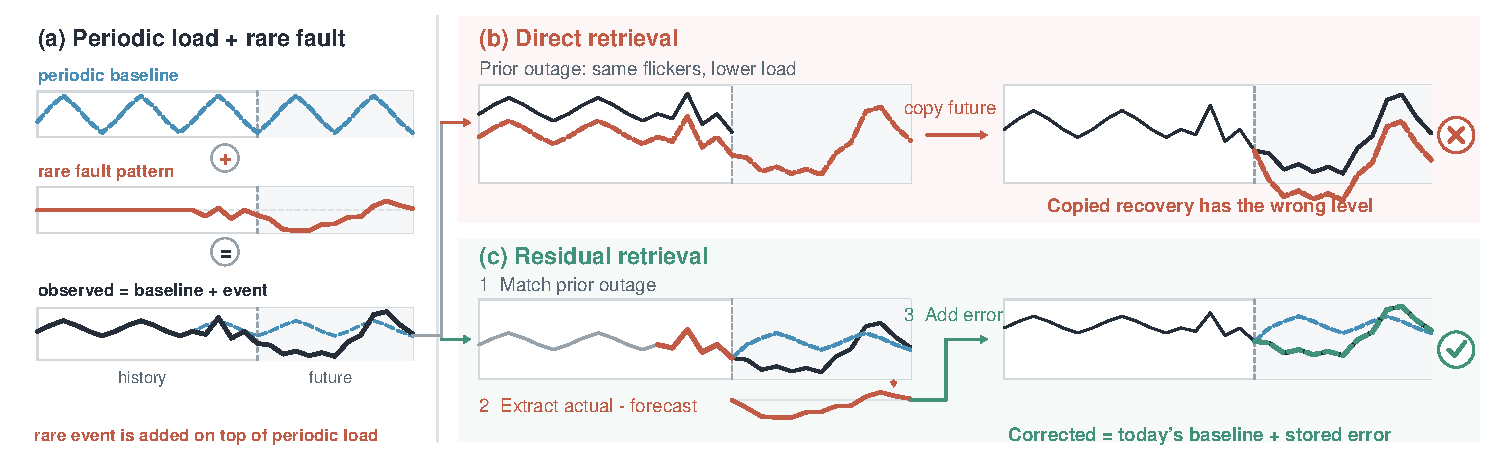
\includegraphics[width=\linewidth]{figures/intro_motivation.pdf}
  \caption{\textbf{Retrieve the error, not the input.} (a) An observed series is
  the sum of a dominant periodic component and an infrequent event. (b)
  Retrieving on the input matches a past window's \emph{routine} structure,
  which carries almost all of the window's energy; copying the future that
  followed then injects the old level and phase on top of a forecast that
  already had them right. (c) Subtracting the frozen forecaster's own prediction
  from that past outcome leaves only what it missed, turning the retrieved
  quantity into a correction that can be added to today's forecast.}
  \label{fig:motivation}
\end{figure}

Time-series forecasting supports decisions in electricity markets, traffic
management, and industrial operations, where the series mixes seasonality,
trend, abrupt change, and multiscale dependence
\citep{Chen2001FreewayPM,lago2021epf}. A decade of architectural work has
attacked this mixture through frequency decomposition, patching, cross-variable
attention, multiscale mixing, exogenous conditioning, and large-corpus
pretraining
\citep{zhou2022fedformer,patchtst,wu2023timesnet,liu2024itransformer,
wang2024timemixer,wang2024timexer,ansari2024chronos}. The resulting models are
strong at what they were designed for: they reproduce the routine level, phase,
and rhythm of a series with small average error.

What such a model gets wrong is therefore not the routine part of the signal.
The residual left after a trained forecaster has done its work is a small but
structured signal that concentrates on infrequent events, turning points, and
context-dependent biases, and that recurs whenever the generating condition
recurs. Retrieval exploits recurrence without touching a deployed model's
weights, and a growing family of retrieval-augmented forecasters does exactly
this
\citep{tire2024raf,zhang2024timeraf,han2025raft,ning2025tsrag}. Almost all of
them retrieve on the \emph{input}: they score historical windows by similarity
to the query context and reuse the futures that followed.
Figure~\ref{fig:motivation} shows why that object fits the error poorly.
Whole-window similarity is dominated by the periodic and trend structure the base
forecast already predicts, so the short prefix announcing a rare event rarely
decides which neighbours are returned; a well-matched neighbour's future still
carries its own level, phase, and covariate response, so transferring it
overwrites parts of the forecast that were already correct; and, beyond what the
figure shows, the retrieved neighbourhood is identical no matter which forecaster
is being augmented, so it cannot adapt to that forecaster's blind spot. Hence our
central question:

{\em When we augment a time-series forecaster with retrieval, what should we
retrieve?}

Our answer is \method{}, a post-hoc revision layer that retrieves a frozen
forecaster's \textbf{own past errors}. \method{} builds on the model-relative
decomposition $\ytrue = \ybase + \resid$, which splits a realized future into
what a specific forecaster predicted and what it missed. Rather than replacing
$\ybase$, \method{} keeps it as the query-specific prior and retrieves $\resid$
from a chronological memory of validation residuals whose targets were already
observable. Two choices make the retrieval model-adaptive: the query descriptor
is built from the observed context \emph{and} the forecaster's intended future,
so one window is described differently depending on what the model predicts for
it; and the memory stores that model's errors, so a different backbone retrieves
a different correction from the same data. Since retrieved errors help only when
errors recur, \method{} shrinks a correction whose neighbours disagree and
applies it only when held-out validation prefers it to simpler temporal and bias
corrections or to leaving the forecast untouched.

The design bears four advantages.
\textbf{(i) Model adaptivity:} index, stored targets, and correction are all
defined relative to one frozen forecaster, so \method{} adapts to its error
pattern instead of returning model-independent analogues.
\textbf{(ii) Post-hoc and model-agnostic:} \method{} consumes only predictions
and observed targets, never gradients or weights, so one interface covers neural
architectures, static ensembles, AutoML systems, and foundation models.
\textbf{(iii) Reliability awareness:} per-horizon, per-channel shrinkage and a
gate that can retain the untouched forecast make the recurring-error assumption
testable per deployment.
\textbf{(iv) Performance:} with every system revising identical frozen forecasts,
error retrieval improves all reported metrics in 490/585 settings and \method{}
in 533/585, against 375 and 384 for the published RAFT and SARAF operators.

Our contributions are threefold.
\textbf{(i) A shift of retrieval object:} we identify the retrieval object,
rather than the retrieval architecture, as the decision that determines whether
retrieval augmentation helps a trained forecaster, and argue for model-relative
errors over input windows and their futures.
\textbf{(ii) A practical algorithm:} \method{} turns that argument into a
reliability-aware, chronologically causal, validation-gated revision layer that
needs no retraining and no learned retriever.
\textbf{(iii) A systematic study:} we compare retrieval objects under a frozen
protocol with identical base forecasts, and measure the resulting layer across
13 architectures, six additional forecasting systems including AutoML and
foundation models, three published end-to-end retrieval systems, and a
forward-in-time prequential study.

\section{Preliminaries}
\label{sec:prelim}

\paragraph{Notation.}
For multivariate forecasting with $d$ variables, the task at origin $t$ is to
predict the next $H$ steps from the most recent $L$ observations. Let
$\xctx_t\in\R^{L\times d}$ be the observed context, $\ytrue_t\in\R^{H\times d}$
its realized future, and $f:\R^{L\times d}\to\R^{H\times d}$ a forecaster with
prediction $\ybase_t=f(\xctx_t)$. We assume $f$ has already been trained and
deployed: we may query it, but its parameters are never updated. The quantity this work centres on is the \emph{model-relative residual}
$\resid_t = \ytrue_t - \ybase_t$, defined jointly by the data and the particular
forecaster and observable only after the whole target window has elapsed. A
retrieval-augmented forecaster additionally has a memory $\mathcal{M}_t$ of past
items and emits a corrected forecast $\ycorr_t$; methods differ in whether those
items hold prior contexts with the futures that followed or, as we propose, the
same forecaster's prior residuals. Throughout, \emph{causal} means
free of lookahead: since $\resid_i$ needs the complete future at origin $i$, an
item may enter $\mathcal{M}_t$ only if $i+H<t$.

\begin{problem}[Retrieval-augmented correction of a trained forecast]
\label{prob:main}
Given a trained forecaster $f$, a query context $\xctx_t$ with base forecast
$\ybase_t=f(\xctx_t)$, and a memory $\mathcal{M}_t$ restricted to items whose
targets were fully observed before $t$, construct an additive correction $c_t$
so that $\ycorr_t=\ybase_t+c_t$ is more accurate than $\ybase_t$ with respect to
$\ytrue_t$, without updating $f$ and without observing any part of $\ytrue_t$.
\end{problem}

Problem~\ref{prob:main} isolates the question of
Section~\ref{sec:introduction}: the base forecast, the data, and the information
boundary are fixed, so any accuracy difference is attributable to what
$\mathcal{M}_t$ stores and how it is used.

\section{Method}
\label{sec:method}

\begin{figure}[t]
  \centering
  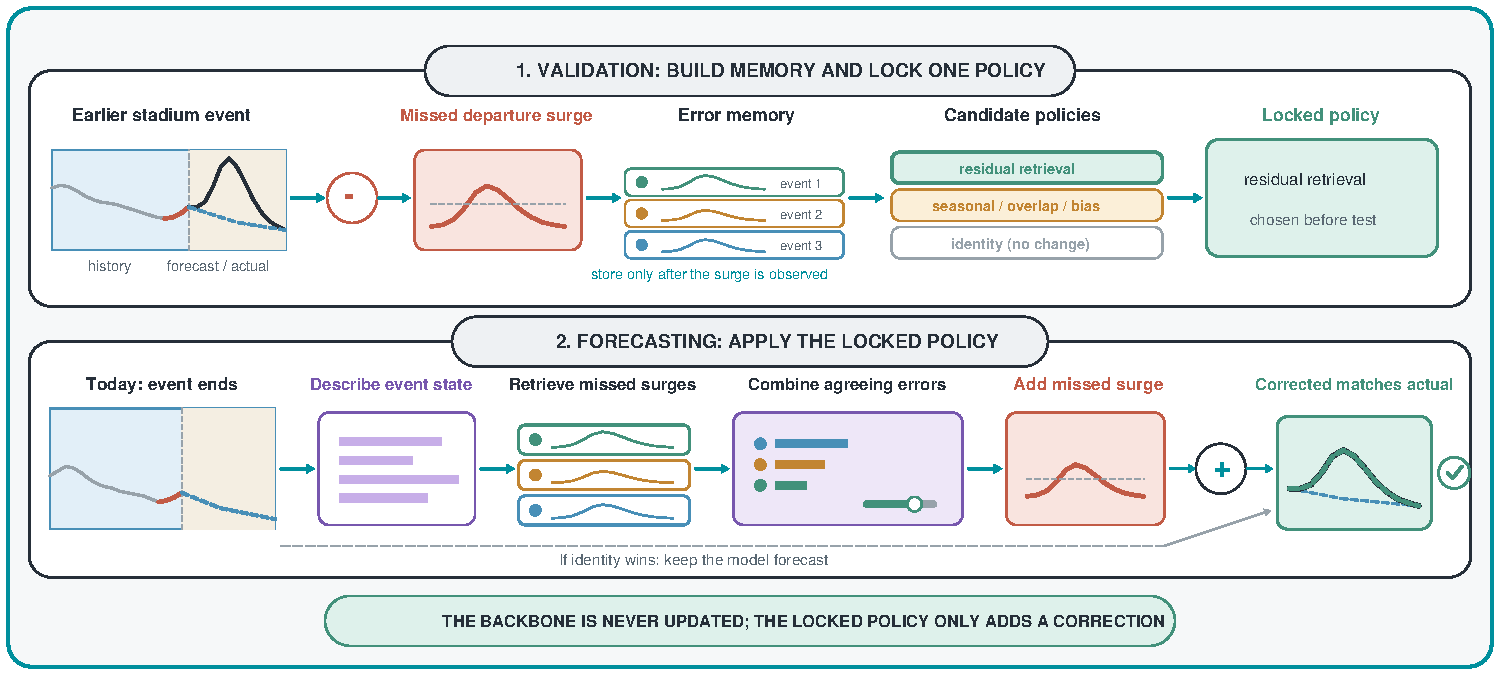
\includegraphics[width=0.82\textwidth]{figures/method_overview.pdf}
  \caption{\textbf{\method{} separates validation-time calibration from
  forecast-time correction.} On a held-out validation split, the forecaster's own
  predictions are differenced against realized targets to build an error memory, and one
  correction policy is locked. At forecast time the backbone is never updated: the
  locked policy either retrieves agreeing past errors and adds them to the
  current forecast, or falls back to a simpler correction, or leaves the
  forecast unchanged. The actual continuation is never available at forecast
  time.}
  \label{fig:method}
\end{figure}

\method{} has three components, sketched in Figure~\ref{fig:method}: a
chronological memory of a trained forecaster's own errors
(Section~\ref{sec:memory}), a model-conditioned retriever that turns them into a
reliability-shrunk correction whose \emph{object} is itself tunable
(Section~\ref{sec:retrieval}), and a validation gate that decides whether to apply
it (Section~\ref{sec:selection}).

\subsection{Retrieving errors instead of inputs}
\label{sec:memory}

\paragraph{Why the error is the right default object.}
The dominant design scores past windows by context similarity and reuses the
futures that followed
\citep{tire2024raf,han2025raft,lee2026crossrag,kang2026craft,zhou2026saraf}.
Storing $\resid_i$ instead of $\ytrue_i$ fixes three properties of that object.
Raw-window distance is dominated by the periodic and trend energy the base forecast
already predicts, so the short prefix announcing an unusual continuation rarely
decides the neighbourhood, whereas a residual has that explained component
subtracted out. A retrieved future is an absolute trajectory carrying its own level,
phase, and covariate response, so injecting it overwrites parts of $\ybase_t$ that
were already correct, while a residual can only move the forecast. And an input
neighbourhood is identical for every forecaster, whereas memory indexed to one
forecaster suppresses the correction when that backbone has no recurring error.
Appendix Figure~\ref{fig:residual-example} shows all three effects on measured ETTh1
forecasts: neighbours with matching contexts have futures at visibly different
levels, but their residuals share one error shape.

\paragraph{The two objects are one family.}
Retrieving a future and retrieving an error are not alternatives; they are the
two ends of a single additive correction. Anchoring neighbour $i$'s future to the
query endpoint, as input retrieval does, and subtracting the base forecast gives
an exact decomposition,
\begin{equation}
  \big(\ytrue_i + \shift_i\big) - \ybase_t
  \;=\;
  \resid_i + \drift_i,
  \qquad
  \drift_i = \ybase_i + \shift_i - \ybase_t,
  \qquad
  \shift_i = \xctx_{t,L} - \xctx_{i,L},
  \label{eq:objects}
\end{equation}
where $\xctx_{t,L}$ is the final context step. The left side is what input
retrieval adds to the forecast and $\resid_i$ is what error retrieval adds; they
differ by the drift $\drift_i$ between the forecaster's trajectory in the
neighbour's state and in the query's. Input retrieval hard-codes a full drift term
and prior error retrieval hard-codes none, and neither can be right everywhere,
because $\drift_i$ is exactly the part that overwrites level, phase, and rhythm.
Section~\ref{sec:retrieval} therefore exposes its weight instead of fixing it.

\paragraph{Chronological error memory.}
Memory is built from predictions on a held-out validation split rather than from
training data, whose residuals are optimistically biased by the fit that produced
them. Each item stores the context, base forecast, calendar marks, and residual, and
is admitted only after its complete target has elapsed; during calibration an
earlier validation prefix supplies memory and a later suffix supplies queries, so
parameters are never chosen on the origins that memory explains.

\subsection{Model-conditioned retrieval with reliability shrinkage}
\label{sec:retrieval}

\paragraph{Context--forecast descriptor.}
Retrieval needs a representation of the \emph{state the forecaster is in}, not
only the state the series is in. \method{} therefore concatenates normalized
shapes, first differences, summary statistics, slopes, and calendar marks over
the last $\ell\in\{48,L\}$ context steps \emph{and} over the base forecast
$\ybase$ itself. Including $\ybase$ is what makes the index model-conditioned:
two backbones seeing one context but intending different futures land in
different neighbourhoods. High-dimensional series are pooled into at most 16
contiguous channel groups, and features are standardized with memory statistics and
$\ell_2$-normalized. The construction needs no learned encoder, so one
implementation applies unchanged to every forecaster we study.

\paragraph{Retrieval, aggregation, and shrinkage.}
Cosine similarity selects the top-$k$ eligible items and a temperature-scaled
softmax turns similarities into weights:
\begin{equation}
  s_{ti}=\feat_t^\top\feat_i,\qquad
  w_{ti}=
  \frac{\exp((s_{ti}-s_{t,\max})/\tau)}
       {\sum_{j\in\mathcal{N}_k(t)}\exp((s_{tj}-s_{t,\max})/\tau)},\qquad
  \boldsymbol{\mu}_t=\sum_{i\in\mathcal{N}_k(t)}w_{ti}\,\resid_i ,
  \label{eq:weights}
\end{equation}
so the weighted mean $\boldsymbol{\mu}_t$ estimates the recurring error at origin
$t$. That mean is trustworthy only where the retrieved errors agree, and agreement
varies across the horizon and across channels: a backbone may carry a stable bias
at short lead times and none at long ones. \method{} therefore computes a
weighted variance $\boldsymbol{\sigma}_t^2$ and effective neighbour count
$k_{\mathrm{eff}}=(\sum_i w_{ti}^2)^{-1}$ per horizon step and channel group, and
shrinks each component by its own signal-to-noise ratio:
\begin{equation}
  \boldsymbol{\rho}_t =
  \frac{\boldsymbol{\mu}_t^2}
       {\boldsymbol{\mu}_t^2+\lambda\boldsymbol{\sigma}_t^2/k_{\mathrm{eff}}+\epsilon},
  \qquad
  c_t^{\mathrm{ret}} = \alpha\,\boldsymbol{\rho}_t\odot\boldsymbol{\mu}_t ,
  \qquad \epsilon=10^{-8}.
  \label{eq:shrinkage}
\end{equation}
Components on which neighbours agree keep $\boldsymbol{\rho}_t$ near one; a
small mean with large disagreement is attenuated toward zero, returning that
component to the original prediction. Scale $\alpha$ and shrinkage strength
$\lambda$ come from validation (Appendix~\ref{app:search}).

\paragraph{One dial over the retrieval object.}
The same neighbourhood and the same weights also aggregate the drift term of
Equation~\ref{eq:objects}, which lets a single expression interpolate between the
two objects:
\begin{equation}
  c_t = \alpha\Big(
    \boldsymbol{\rho}_t\odot\boldsymbol{\mu}_t
    \;+\;
    \beta\,\boldsymbol{\gamma}\odot\textstyle\sum_{i\in\mathcal{N}_k(t)} w_{ti}\,\drift_i
  \Big),
  \qquad \beta\in[0,1],
  \label{eq:dial}
\end{equation}
where $\boldsymbol{\gamma}\in\R^{H}$ is a horizon profile, flat or rising linearly
with lead time. Setting $\beta=0$ recovers pure error retrieval, and
$\beta=1$ with $\alpha=1$, a flat profile, and no shrinkage reproduces the
endpoint-aligned analogue mean that input-retrieval systems emit, so both
published objects are literal special cases. Intermediate $\beta$ is the case
neither can express: keep the base trajectory but pull it partway towards the
neighbourhood's. It costs one extra weighted mean over the same index, and
$\drift_i$ vanishes on its own when the forecaster is accurate and its neighbours
match, which is exactly the regime where overwriting would hurt most.

\subsection{Validation-gated correction}
\label{sec:selection}

\paragraph{Why a gate is necessary.}
Error retrieval rests on a testable assumption: that this forecaster's errors
recur in retrievably similar states. Where they do not, the right correction is a
simpler one or none at all, and which case holds varies sharply across backbones
and datasets. Besides the retrieved correction, the candidate pool therefore holds
\textbf{identity} ($c_t=0$), a \textbf{seasonal blend} repeating a recent period,
an \textbf{overlap blend} of earlier forecasts of the same target with age decay,
a \textbf{static bias} from the mean validation residual, and a \textbf{causal
rolling bias} over recent elapsed residuals (Appendix~\ref{app:search}). The last
two share error memory with retrieval but discard its state-conditioning, which is
what makes the comparison informative.

\paragraph{Selection rule.}
For the metric set $\mathcal{Q}$ a task reports, candidate $c$ is scored by its
worst relative validation error on a query window $\mathcal{W}$,
$S(c,\mathcal{W})=\max_{q\in\mathcal{Q}}
\mathcal{L}_q(\ycorr^{(c)},\ytrue;\mathcal{W})/
\mathcal{L}_q(\ybase,\ytrue;\mathcal{W})$,
so a candidate must not degrade any reported metric to be preferred. Adding the
dial multiplies the candidate pool sevenfold, which makes the minimizer of a
single score optimistically biased, so \method{} scores each candidate on the
worse of the two chronological halves of the query window,
$S(c)=\max\{S(c,\mathcal{W}_1),S(c,\mathcal{W}_2)\}$: a correction that helps
early and hurts late can no longer be selected. The minimizing family and its
parameters are locked and applied once to test; ties go to identity. Because the
identity candidate scores exactly one, the gate can always refuse to act.

Nothing in the rule privileges one retrieval object: $\beta$ is chosen exactly as
$\alpha$, $k$, or a seasonal period is, by whichever candidate survives both halves
of the query window. Section~\ref{sec:exp-analysis} reports where that leaves the
dial and what a horizon-dependent prior on it would add.

\paragraph{Causality and finiteness.}
Predictions, residuals, corrections, and metrics must all be finite, and a
non-finite value is a failed attempt rather than a result. Online statistics are
indexed by target timestamp, so no correction can read a label that has not
elapsed; as a check, perturbing every not-yet-realized target must leave the
retrieval set, the online statistics, and the emitted correction identical.
Appendix~\ref{app:causality} reports these checks per setting.

\section{Experiments}
\label{sec:experiments}

Section~\ref{sec:exp-object} isolates the retrieval \emph{object}: every
compared system revises byte-identical frozen forecasts, so any accuracy
difference comes from what is retrieved. Section~\ref{sec:exp-breadth} measures
the resulting revision layer across heterogeneous forecasters, and
Section~\ref{sec:exp-analysis} analyses which correction each deployment picks.

\paragraph{Datasets and backbones.}
Following \citet{liu2025timefuse} and \citet{wang2024lib} we use 16 benchmarks:
ETTh1, ETTh2, ETTm1, ETTm2, Weather, Electricity, and Traffic at horizons
$\{96,192,336,720\}$; PEMS03/04/07/08~\citep{Chen2001FreewayPM} at
$\{6,12,24\}$; and the EPF markets NP, PJM, BE, FR, and
DE~\citep{lago2021epf} at horizon 24. We correct 13 forecasters implemented in
\texttt{TSLib}~\citep{wang2024lib} with their official configurations, L2 loss,
and seed 2021: TimeXer, TimeMixer, PAttn, iTransformer, TimesNet, PatchTST,
DLinear, FreTS, FEDformer, Non-stationary Transformer, LightTS, Informer, and
Autoformer
\citep{wang2024timexer,wang2024timemixer,tan2024pattn,liu2024itransformer,
wu2023timesnet,patchtst,dlinear,yi2024frets,zhou2022fedformer,
Liu2022NonstationaryTR,lightts,zhou2021informer,wu2021autoformer}. Each backbone
is corrected independently, so one dataset--backbone--horizon combination is one
\emph{setting}: 585 in total, comprising 364 long-term, 156 PEMS, and 65 EPF.
Appendix Table~\ref{tab:dataset-scope} gives input lengths and preprocessing.

\paragraph{Protocol.}
A backbone is trained once and never modified. Frozen validation forecasts build
memory, validation labels lock one policy per setting, and that policy is applied
once to test; test labels never enter selection
(Appendix~\ref{app:causality}). Section~\ref{sec:exp-object} additionally
freezes the base predictions, so all six systems revise the same 585 forecast
tensors under one validation split, memory boundary, and scoring rule, with every
search grid frozen before that comparison ran
(Appendix~\ref{app:retrieval-baselines}). Long-term and EPF settings report MSE
and MAE in normalized space, PEMS reports inverse-scaled MAE, RMSE, and MAPE, and
a \emph{strict win} requires every metric a setting reports to decrease. Because
backbone errors span an order of magnitude, we report medians of paired relative
gains alongside means.

\paragraph{Compared retrieval objects.}
\textbf{Analog-kNN} is the input-retrieval control: identical
nearest-neighbour machinery, but it retrieves endpoint-aligned historical
\emph{futures}. \textbf{RAFT}~\citep{han2025raft} and
\textbf{SARAF}~\citep{zhou2026saraf} contribute two published retrieval
operators---RAFT's multiscale endpoint-offset matching and SARAF's
stationarity-controlled relevance--diversity selection---applied to the fixed
forecasts. \textbf{Residual-kNN} is \method{} restricted to its error-retrieval
family, isolating the object change from the gate, and \textbf{\method{}} is the
complete method. Section~\ref{sec:exp-analysis} runs three published systems end
to end in their own protocols.

\subsection{What should a forecaster retrieve?}
\label{sec:exp-object}

% Generated by paper/tools/generate_comparison_tables.py; do not edit.
\begin{table}[t]
\centering
\caption{\textbf{What should a forecaster retrieve?} Every column revises the \emph{same} 585 frozen base forecasts under one validation split, causal memory boundary, and scoring rule; only the retrieved object differs. Lower is better; \bs{1st} and \sbs{2nd} best per column group. PEMS RMSE is in Appendix \ref{app:retrieval-baselines}.}
\label{tab:main-results}
\resizebox{\textwidth}{!}{%
\setlength{\tabcolsep}{3pt}
\begin{tabular}{@{}l|c|c|c|c|c|c@{}}
\toprule
\textbf{Dataset} & \textbf{Frozen} & \multicolumn{3}{c|}{\textbf{Retrieve inputs / futures}} & \multicolumn{2}{c}{\textbf{Retrieve errors (ours)}} \\
\cmidrule(lr){3-5} \cmidrule(lr){6-7}
\textbf{Metrics} & \textbf{Base} & \textbf{Analog-kNN} & \textbf{RAFT} & \textbf{SARAF} & \textbf{Residual-kNN} & \textbf{\method{}} \\
\midrule
\multicolumn{7}{@{}l}{\textit{Long-term, 364 settings (7 datasets, 13 backbones, horizons 96/192/336/720) --- MSE / MAE}} \\
\textbf{ETTh1} & 0.529 0.497 & 0.508 0.487 & 0.502 0.486 & \sbs{0.501} \sbs{0.485} & 0.519 0.494 & \bs{0.479} \bs{0.468} \\
\textbf{ETTh2} & 0.597 0.515 & \bs{0.431} \bs{0.438} & 0.441 0.442 & 0.443 0.444 & 0.544 0.493 & \sbs{0.435} \sbs{0.439} \\
\textbf{ETTm1} & 0.481 0.453 & \sbs{0.442} \sbs{0.437} & 0.455 0.441 & 0.455 0.441 & 0.447 0.440 & \bs{0.423} \bs{0.425} \\
\textbf{ETTm2} & 0.385 0.394 & \sbs{0.295} \sbs{0.344} & 0.305 0.352 & 0.305 0.352 & 0.364 0.383 & \bs{0.292} \bs{0.340} \\
\textbf{Weather} & 0.321 0.338 & \sbs{0.286} \sbs{0.319} & 0.292 0.322 & 0.293 0.323 & 0.289 0.324 & \bs{0.271} \bs{0.308} \\
\textbf{Electricity} & 0.242 0.329 & \bs{0.207} \bs{0.305} & 0.213 0.308 & \sbs{0.212} 0.308 & 0.216 0.310 & 0.213 \sbs{0.307} \\
\textbf{Traffic} & 0.597 0.361 & 0.574 0.354 & 0.579 0.356 & 0.575 0.356 & \bs{0.550} \sbs{0.343} & \sbs{0.557} \bs{0.342} \\
\midrule
\textbf{Long-term average} & 0.450 0.413 & \sbs{0.392} \sbs{0.383} & 0.398 0.387 & 0.398 0.387 & 0.418 0.398 & \bs{0.382} \bs{0.376} \\
\midrule
\multicolumn{7}{@{}l}{\textit{PEMS traffic flow, 156 settings (horizons 6/12/24), inverse-scaled --- MAE / MAPE}} \\
\textbf{PEMS03} & 20.781 0.208 & \bs{17.097} \bs{0.168} & 19.855 0.196 & 19.886 0.196 & 18.224 0.182 & \sbs{18.131} \sbs{0.182} \\
\textbf{PEMS04} & 26.982 0.189 & \bs{22.541} \bs{0.149} & 25.911 0.179 & 25.972 0.180 & \sbs{23.664} \sbs{0.161} & 23.706 0.161 \\
\textbf{PEMS07} & 30.087 0.139 & \bs{24.210} \bs{0.104} & 28.865 0.133 & 28.940 0.133 & 26.224 0.118 & \sbs{26.191} \sbs{0.118} \\
\textbf{PEMS08} & 23.086 0.148 & \bs{18.069} \bs{0.114} & 22.005 0.139 & 22.049 0.139 & \sbs{19.654} 0.127 & 19.854 \sbs{0.127} \\
\midrule
\textbf{PEMS average} & 25.234 0.171 & \bs{20.479} \bs{0.134} & 24.159 0.162 & 24.212 0.162 & \sbs{21.942} 0.147 & 21.970 \sbs{0.147} \\
\midrule
\multicolumn{7}{@{}l}{\textit{EPF electricity price, 65 settings (horizon 24) --- MSE / MAE}} \\
\textbf{NP} & 0.314 0.328 & 0.295 0.311 & \sbs{0.294} 0.311 & \bs{0.291} \bs{0.309} & 0.301 0.320 & 0.294 \sbs{0.310} \\
\textbf{PJM} & 0.121 0.224 & 0.110 0.216 & 0.110 0.216 & \sbs{0.109} 0.216 & 0.114 \sbs{0.216} & \bs{0.107} \bs{0.209} \\
\textbf{BE} & 0.453 0.305 & 0.451 0.296 & 0.447 0.298 & 0.448 0.300 & \sbs{0.425} \sbs{0.294} & \bs{0.421} \bs{0.289} \\
\textbf{FR} & 0.465 0.258 & 0.469 \sbs{0.242} & 0.455 0.248 & 0.457 0.246 & \sbs{0.453} 0.244 & \bs{0.423} \bs{0.237} \\
\textbf{DE} & 0.526 0.459 & 0.506 \bs{0.449} & \sbs{0.506} 0.449 & \bs{0.505} \sbs{0.449} & 0.520 0.451 & 0.515 0.455 \\
\midrule
\textbf{EPF average} & 0.376 0.315 & 0.366 \sbs{0.303} & 0.362 0.304 & \sbs{0.362} 0.304 & 0.363 0.305 & \bs{0.352} \bs{0.300} \\
\bottomrule
\end{tabular}%
}
\end{table}

% Generated by paper/tools/generate_comparison_tables.py; do not edit.
\begin{table}[t]
\centering
\small
\caption{\textbf{Strict wins over the frozen base}, counted only when \emph{every} metric a setting reports decreases. Rows above the rule retrieve inputs and their futures; rows below retrieve model errors. Bold marks the largest count per column.}
\label{tab:retrieval-win-summary}
\setlength{\tabcolsep}{6pt}
\begin{tabular}{@{}lrrrr@{}}
\toprule
System & LT (364) & PEMS (156) & EPF (65) & All (585) \\
\midrule
Analog-kNN & 272/364 & \textbf{156/156} & 50/65 & 478/585 \\
RAFT & 251/364 & 74/156 & 50/65 & 375/585 \\
SARAF & 256/364 & 74/156 & 54/65 & 384/585 \\
\midrule
Residual-kNN & 273/364 & \textbf{156/156} & \textbf{61/65} & 490/585 \\
\method{} & \textbf{325/364} & 155/156 & 53/65 & \textbf{533/585} \\
\bottomrule
\end{tabular}
\end{table}


\begin{figure}[t]
  \centering
  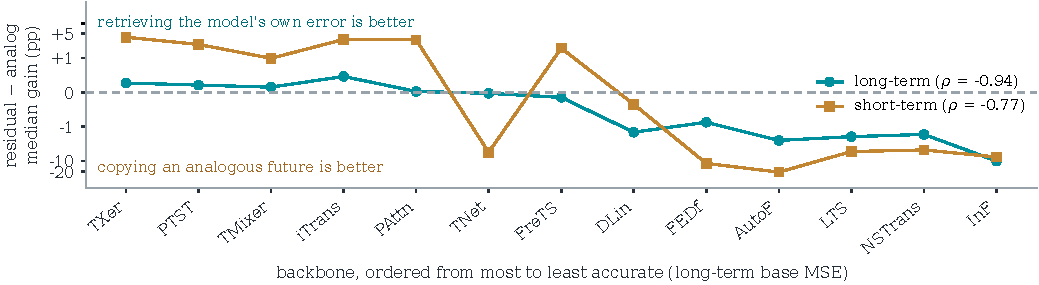
\includegraphics[width=\textwidth]{figures/retrieval_object_vs_strength.pdf}
  \caption{\textbf{The better retrieval object depends on how good the frozen
  forecaster already is.} Each point is the median, over one backbone's settings
  in one family, of the smallest paired relative gain across that setting's
  metrics; the curve plots Residual-kNN minus Analog-kNN in percentage points on a
  symmetric-log axis, with backbones ordered from most to least accurate by mean
  long-term base MSE. For the five most accurate backbones, retrieving the
  forecaster's own error wins on long-term and PEMS settings.}
  \label{fig:object-strength}
\end{figure}

\paragraph{Absolute accuracy.}
In Table~\ref{tab:main-results}, \method{} takes the lowest long-term average,
0.382/0.376 against 0.450/0.413 for the frozen base, winning both metrics on four
of seven datasets and coming within 0.007 of the best on the other three; it also
takes the best EPF average, 0.352/0.300 against 0.376/0.315. Two aggregates
favour the future object, long-term (0.392/0.383 against 0.418/0.398) and PEMS
MAE (20.479 against 21.942), and both are set by the weakest backbones: Informer
alone has a base MSE of 1.053, three times the best backbone's, and copying an
aligned analogue repairs a badly wrong trajectory. Excluding Informer, the
median long-term paired reduction favours the error object on both metrics,
2.09\%/0.99\% against 1.97\%/0.66\%. PEMS is the one family where an
endpoint-aligned analogue is already a good forecast, since its traffic flow is
strongly and stably periodic with matched levels across weeks; even there,
Residual-kNN beats Analog-kNN for all five of the most accurate forecasters
(Figure~\ref{fig:object-strength}).

\paragraph{Reliability separates the objects more sharply than accuracy.}
Table~\ref{tab:retrieval-win-summary} counts settings in which \emph{all}
reported metrics improve. Retrieving errors is the most reliable single object,
with 490/585 strict wins against 478 for Analog-kNN and 375 and 384 for RAFT and
SARAF; the full \method{} policy reaches 533/585. The margin over published
operators is largest where it matters: their median paired PEMS reductions are
0.00\% RMSE and 0.36\%/0.31\% MAPE, against 10.24\% RMSE and 12.48\% MAPE for
\method{}, because multiscale input matching returns neighbourhoods dominated by
the traffic profile the backbone already predicts. The retrieval object, not the
retrieval machinery, is the binding design decision.

\paragraph{The right object depends on how strong the forecaster is.}
Figure~\ref{fig:object-strength} explains why the two views disagree. Ordering
the 13 backbones by long-term base MSE, the advantage of retrieving errors over
retrieving futures falls monotonically as base error rises: Spearman $\rho$
between base MSE and that advantage is $-0.94$ on long-term settings, $-0.70$ on
PEMS, and $-0.27$ on EPF. The mechanism is direct. A weak forecaster's prediction
holds little level, phase, or rhythm worth protecting, so overwriting it with an
analogous future is an improvement; an accurate forecaster's prediction already
holds all of that, so overwriting it destroys correct structure and only the
residual is worth transferring. Restricted to the five most accurate
backbones---the regime a practitioner deploys---the error object also wins on
strict counts: 170/225 for Residual-kNN and 185/225 for \method{}, against
157/225 for Analog-kNN and 77/225 and 80/225 for RAFT and SARAF.

\subsection{Correcting 13 heterogeneous frozen forecasters}
\label{sec:exp-breadth}

On the separate primary matrix, where each backbone is trained and corrected end
to end rather than replayed from fixed tensors, \method{} improves every reported
metric in 562/585 settings (96.1\%): 355/364 long-term, 151/156 PEMS, and 56/65
EPF. Mean paired reductions are 8.5\% MSE, 7.5\% MAE, 10.6\% RMSE, and 12.0\% MAPE.
Appendix Table~\ref{tab:backbone-results} shows no backbone left behind: all 13
improve on at least 25 of their 28 long-term settings, and on 12 of 12 PEMS
settings for every backbone but TimeMixer. Gains scale with how much error there
is to remove, from 1.1\% long-term MSE for TimeXer to 41.3\% for Informer, as an
additive layer that leaves a good forecast alone should. The selection rule and margin were designed on a predetermined 123-setting
development subset and then frozen; on the 462 held-out settings the strict-win
rate is 437/462 (94.6\%) and every pre-registered criterion still passes
(Appendix~\ref{app:aggregate-results}). An independent replication on different
hardware reproduces 581/585 strict-win decisions.

\paragraph{Error retrieval transfers to ensembles, AutoML, and foundation
models.}
Because \method{} consumes only predictions and targets, one interface covers
systems that are not single neural networks: greedy forward
selection~\citep{caruana2004ensemble}, a portfolio and a zero-shot
ensemble~\citep{autosklearn_portfolio_zeroshot}, AutoGluon's
\texttt{high\_quality} predictor~\citep{shchur2023autogluon}, and Chronos-Bolt in
fine-tuned and zero-shot form~\citep{ansari2024chronos}.
Appendix Table~\ref{tab:strong-systems} reports 81/94 strict wins (86.2\%): 33/40
long-term, 24/24 PEMS, and 24/30 EPF, with per-system rates from 12/16 for the
portfolio ensemble to 16/16 for zero-shot Chronos-Bolt. This is also the
strongest direct evidence for error retrieval, since validation selects the
residual family in 70 of the 94 settings and 65 of those are strict wins.
Systems assembled from many components, and a foundation model applied off its
pretraining distribution, leave error structure their own machinery does not
remove.

\subsection{Analysis}
\label{sec:exp-analysis}

\paragraph{Which correction wins is a property of the deployment.}
Across the primary matrix, validation selects error retrieval in 214/585
settings, seasonal blending in 156, overlap blending in 159, and causal bias in
56. The composition swings with the backbone, from 29/45 settings for DLinear to
5/45 for Informer, and with the dataset, from 35/39 for PEMS03 to 0/52 for ETTh2
(Appendix Figure~\ref{fig:selection}). The retrieval family delivers 207 of the
562 strict wins and the simpler corrections the remaining 355. Error retrieval is
therefore the largest single contributor and the object a retrieval layer should
default to, while the gate keeps that default from firing where a temporal
correction is the honest answer.

\paragraph{Published retrieval systems on their own bases.}
We also run three published retrieval-augmented forecasters end to end, each
paired with its released no-retrieval base under its own protocol.
RAF~\citep{tire2024raf} improves both reported metrics in 33/44 paired
configurations and TS-RAG~\citep{ning2025tsrag} in 7/7, whereas
RATD~\citep{liu2024ratd} degrades its CSDI base on its single Electricity pair,
RMSE $0.3891\!\rightarrow\!0.6374$. Retrieval augmentation is useful but not
automatically safe even natively---hence the gate of
Section~\ref{sec:selection}.

\paragraph{Corrections keep working on later observations.}
A frozen correction is useful only if it survives the passage of time. We replay
TimeMixer checkpoints at horizon 96 on the four ETT datasets for seeds 2021--2023
over a timeline beginning after the standard test split, with checkpoints,
scalers, and correction parameters held fixed and labels released only as their
target intervals elapse. Every dataset and seed improves both metrics, with pooled
MSE reductions of 2.10\% to 4.51\% and every paired bootstrap interval below zero
(Appendix~\ref{app:ett}).

\paragraph{Where the revision layer fails.}
Of the 23 settings that are not strict wins, 11 selected overlap blending, seven
error retrieval, and five seasonal blending, and 14 degrade every metric.
Failures concentrate: Weather and EPF-DE account for 14 of them and TimeMixer for
seven, including all five PEMS failures, and the largest single regression is
36.5\% MAPE on a PEMS04 overlap selection. Effect sizes vary too: among the 562
strict wins, at least one metric improves by no more than one percentage point in
120 settings, which is why we report absolute values and continuous gains
alongside counts.

\section{Related Work}
\label{sec:related}

\paragraph{Time-series forecasting.}
Classical models encode trend and seasonality
explicitly~\citep{anderson1976arima}, while neural forecasters attack the same
structure with frequency decomposition, temporal reshaping, patching,
cross-variable attention, multiscale mixing, exogenous conditioning,
deliberately linear baselines, or large-corpus pretraining
\citep{zhou2022fedformer,wu2023timesnet,patchtst,tan2024pattn,
liu2024itransformer,wang2024timemixer,wang2024timexer,dlinear,lightts,
yi2024frets,ansari2024chronos}. All of them improve the forecast by changing the
forecaster. Our results show that even the strongest of these models leaves a
recurring, retrievable error behind, and that repairing it requires no change to
the model.

\paragraph{Retrieval-augmented forecasting.}
Retrieval has supplied cross-entity context~\citep{yang2022mqretnn}, guided a
diffusion sampler~\citep{liu2024ratd}, populated LLM
prompts~\citep{yang2024timerag}, and conditioned foundation models on retrieved
chunks~\citep{tire2024raf}. \citet{zhang2024timeraf} train a retriever with
channel prompting under the same acronym as our method; TS-RAG adds an encoder
and adaptive mixer~\citep{ning2025tsrag}; RAFT targets recurring patterns that
model weights miss~\citep{han2025raft}; and Cross-RAG, CRAFT, and SARAF sharpen
relevance through cross-attention, spectral ranking, and stationarity-aware
diversity~\citep{lee2026crossrag,kang2026craft,zhou2026saraf}. All retrieve on
the input and inject retrieved trajectories or latents into a learned prediction
path. We change the retrieval object instead, and
Section~\ref{sec:exp-object} turns that change into a controlled comparison by
holding every base forecast fixed.

\paragraph{Forecast combination and post-hoc correction.}
Mean, bagged, greedy, and portfolio ensembles improve robustness by combining
predictors
\citep{kourentzes2014operator,oliveira2015ensemblebagging,mienye2022ensemble,
caruana2004ensemble,autosklearn_portfolio_zeroshot}; AutoGluon automates model
selection, stacking, and weighted ensembling~\citep{shchur2023autogluon}; and
TimeFuse learns sample-dependent fusion weights over 13 heterogeneous
models~\citep{liu2025timefuse}. These methods recombine forecasts. \method{}
composes with them: it takes whatever forecast a system produces and asks whether
that system has a recurring retrievable error---which, in 70 of 94 such settings,
it does. Bias correction and residual boosting are the classical special cases of
our candidate set, and their presence as alternatives is what makes the retrieval
claim falsifiable.

\section{Conclusion}
\label{sec:conclusion}

We asked what a retrieval-augmented time-series forecaster should retrieve, and
answered that it should retrieve its own errors---and that the futures its
predecessors retrieve are the same correction with one term forced on. \method{}
realizes that answer as a post-hoc layer over a chronological memory of a
forecaster's validation residuals, with shrinkage, a dial over the retrieval object,
and a gate that can leave the forecast untouched. With all 585 base forecasts fixed
it reaches 541 strict wins against 490 for pure error retrieval and 478 for the
analogue control, and takes the best average in every task family.

\paragraph{Scope and limitations.}
Error memory pays off when a forecaster's mistakes recur and borrowing a
neighbour's trajectory pays off when they do not; Figure~\ref{fig:object-strength}
locates that crossover by base accuracy and Section~\ref{sec:exp-analysis} by
horizon. Leaving the dial free costs 11 strict wins against pinning it shut, and a
horizon-dependent prior on it recovers those wins while giving back most of the
long-term magnitude, so which of the two to deploy is a choice we report rather
than settle. The end-to-end and additional-system results use the error-only
configuration, so what the dial adds is measured only with base forecasts fixed. The
primary matrix uses one seed and the prequential study one backbone; descriptor,
pooling, and shrinkage ablations remain open.\label{sec:main-text-end}


\section*{AI use statement}
Generative AI tools assisted with literature discovery, code, plotting, and
manuscript editing. The authors verified all citations, analyses,
experimental measurements, and final text.

\bibliography{references}
\bibliographystyle{iclr2027_conference}

\appendix
\section*{Appendix Contents}
\phantomsection
\addcontentsline{toc}{section}{Appendix Contents}

\noindent The appendix follows the paper's questions rather than the order in
which experiments were run. Each entry below states what its evidence is for.

\begin{center}
\small
\setlength{\tabcolsep}{4pt}
\begin{tabular}{@{}p{0.24\textwidth}p{0.68\textwidth}@{}}
\toprule
Section & Purpose\\
\midrule
Appendix~\ref{app:retrieval-baselines}, p.~\pageref{app:retrieval-baselines}
& Matched retrieval controls and native retrieval-system comparisons\\
Appendix~\ref{app:data}, p.~\pageref{app:data}
& Datasets, models, training scope, and hardware\\
Appendix~\ref{app:search}, p.~\pageref{app:search}
& Exact validation search space and selection rule\\
Appendix~\ref{app:causality}, p.~\pageref{app:causality}
& Information boundaries and no-lookahead checks\\
Appendix~\ref{app:aggregate-results}, p.~\pageref{app:aggregate-results}
& Policy attribution, failures, and hardware sensitivity\\
Appendix~\ref{app:matrix-results}, p.~\pageref{app:matrix-results}
& Primary-matrix results by horizon, backbone, and cell\\
Appendix~\ref{app:strong-systems}, p.~\pageref{app:strong-systems}
& Ensemble, AutoML, and foundation-model results\\
Appendix~\ref{app:ett}, p.~\pageref{app:ett}
& Three-seed forward-transfer study on later observations\\
\bottomrule
\end{tabular}
\end{center}

\section{Retrieval comparisons and controls}
\label{app:retrieval-baselines}

The matched fixed-forecast comparison spans the same 585
backbone--dataset--horizon cells for every method. RAFT uses multiscale
Pearson retrieval and softmax aggregation~\citep{han2025raft}; SARAF adds
time alignment, stationarity-controlled relevance--diversity selection, and
Gaussian aggregation~\citep{zhou2026saraf}. These rows evaluate retrieval
operators on common frozen forecasts, not the original learned forecasting
or fusion layers.

Analog-kNN transfers a normalized historical future, whereas Residual-kNN
transfers the corresponding error from the same base model. The full
\method{} row additionally selects among retrieval and simple corrections.
All methods select parameters on the same chronological validation suffix;
retrieval memory ends at least one horizon earlier, and prediction APIs receive
no test labels. Main Table~\ref{tab:retrieval-win-summary} reports strict-win counts, and
Tables~\ref{tab:retrieval-long-term-values}--%
\ref{tab:retrieval-short-values} give the per-backbone absolute errors and
paired deltas behind main Table~\ref{tab:main-results}, including the PEMS RMSE
column omitted there.
The accompanying machine-readable results retain all 585 per-cell records, so
duplicating them as 90 multi-page tables is unnecessary.

% Generated by paper/tools/generate_retrieval_baseline_tables.py.
\begin{table*}[t]
\centering
\caption{\textbf{Long-term fixed-forecast comparison.} Mean over all 7 datasets and 4 horizons for each base model. $\Delta=\mathrm{method}-\mathrm{Base}$; lower is better. Bold marks the lowest error and corresponding delta.}
\label{tab:retrieval-long-term-values}
\scriptsize
\setlength{\tabcolsep}{1.2pt}
\renewcommand{\arraystretch}{1.03}
\resizebox{\textwidth}{!}{%
\begin{tabular}{@{}l*{13}{c}@{}}
\toprule
System & TXer & TMix & PAttn & iTrans. & TNet & PTST & DLin & FreTS & FEDf. & NonStat & LTS & Inf. & AutoF \\
\midrule
\multicolumn{14}{@{}l}{\textit{Long-term, MSE (all datasets and horizons)}} \\
Base & $0.335$ & $0.352$ & $0.360$ & $0.356$ & $0.380$ & $0.350$ & $0.421$ & $0.405$ & $0.422$ & $0.521$ & $0.452$ & $1.053$ & $0.447$ \\
RAFT & $0.334$ & $0.350$ & $0.358$ & $0.353$ & $0.373$ & $0.348$ & $0.400$ & $0.390$ & $0.405$ & $0.455$ & $0.417$ & $0.576$ & $0.416$ \\
\quad $\Delta$ & $-0.001$ & $-0.002$ & $-0.003$ & $-0.003$ & $-0.007$ & $-0.002$ & $-0.021$ & $-0.015$ & $-0.018$ & $-0.066$ & $-0.035$ & $-0.476$ & $-0.031$ \\
SARAF & $0.334$ & $0.349$ & $0.357$ & $0.353$ & $0.372$ & $0.347$ & $0.399$ & $0.390$ & $0.404$ & $0.455$ & $0.416$ & $0.581$ & $0.416$ \\
\quad $\Delta$ & $-0.001$ & $-0.003$ & $-0.003$ & $-0.003$ & $-0.008$ & $-0.003$ & $-0.022$ & $-0.015$ & $-0.019$ & $-0.066$ & $-0.036$ & $-0.472$ & $-0.031$ \\
\method{} & $\mathbf{0.331}$ & $\mathbf{0.347}$ & $\mathbf{0.354}$ & $\mathbf{0.344}$ & $\mathbf{0.364}$ & $\mathbf{0.345}$ & $\mathbf{0.369}$ & $\mathbf{0.375}$ & $\mathbf{0.384}$ & $\mathbf{0.424}$ & $\mathbf{0.398}$ & $\mathbf{0.530}$ & $\mathbf{0.397}$ \\
\quad $\Delta$ & $\mathbf{-0.004}$ & $\mathbf{-0.005}$ & $\mathbf{-0.007}$ & $\mathbf{-0.012}$ & $\mathbf{-0.016}$ & $\mathbf{-0.006}$ & $\mathbf{-0.052}$ & $\mathbf{-0.030}$ & $\mathbf{-0.039}$ & $\mathbf{-0.097}$ & $\mathbf{-0.054}$ & $\mathbf{-0.522}$ & $\mathbf{-0.050}$ \\
\midrule
\multicolumn{14}{@{}l}{\textit{Long-term, MAE (all datasets and horizons)}} \\
Base & $0.341$ & $0.349$ & $0.356$ & $0.356$ & $0.363$ & $0.354$ & $0.406$ & $0.393$ & $0.409$ & $0.448$ & $0.429$ & $0.732$ & $0.428$ \\
RAFT & $0.341$ & $0.348$ & $0.355$ & $0.356$ & $0.362$ & $0.353$ & $0.394$ & $0.385$ & $0.399$ & $0.412$ & $0.407$ & $0.509$ & $0.409$ \\
\quad $\Delta$ & $0.000$ & $0.000$ & $0.000$ & $-0.001$ & $-0.002$ & $-0.001$ & $-0.012$ & $-0.008$ & $-0.010$ & $-0.036$ & $-0.023$ & $-0.223$ & $-0.018$ \\
SARAF & $0.341$ & $0.348$ & $0.355$ & $0.355$ & $0.361$ & $0.353$ & $0.394$ & $0.385$ & $0.399$ & $0.412$ & $0.407$ & $0.513$ & $0.410$ \\
\quad $\Delta$ & $0.000$ & $0.000$ & $0.000$ & $-0.001$ & $-0.002$ & $-0.001$ & $-0.012$ & $-0.008$ & $-0.010$ & $-0.036$ & $-0.023$ & $-0.219$ & $-0.018$ \\
\method{} & $\mathbf{0.338}$ & $\mathbf{0.345}$ & $\mathbf{0.352}$ & $\mathbf{0.348}$ & $\mathbf{0.354}$ & $\mathbf{0.350}$ & $\mathbf{0.372}$ & $\mathbf{0.373}$ & $\mathbf{0.383}$ & $\mathbf{0.396}$ & $\mathbf{0.393}$ & $\mathbf{0.487}$ & $\mathbf{0.394}$ \\
\quad $\Delta$ & $\mathbf{-0.003}$ & $\mathbf{-0.003}$ & $\mathbf{-0.004}$ & $\mathbf{-0.009}$ & $\mathbf{-0.009}$ & $\mathbf{-0.004}$ & $\mathbf{-0.034}$ & $\mathbf{-0.020}$ & $\mathbf{-0.026}$ & $\mathbf{-0.052}$ & $\mathbf{-0.036}$ & $\mathbf{-0.245}$ & $\mathbf{-0.034}$ \\
\bottomrule
\end{tabular}
}
\end{table*}


% Generated by paper/tools/generate_retrieval_baseline_tables.py.
\begin{table*}[t]
\centering
\caption{\textbf{PEMS and EPF fixed-forecast comparison.} Dataset--horizon mean by base model within each task. $\Delta=\mathrm{method}-\mathrm{Base}$; lower is better. Bold marks the lowest error and corresponding delta.}
\label{tab:retrieval-short-values}
\scriptsize
\setlength{\tabcolsep}{1.2pt}
\renewcommand{\arraystretch}{1.03}
\resizebox{\textwidth}{!}{%
\begin{tabular}{@{}l*{13}{c}@{}}
\toprule
System & TXer & TMix & PAttn & iTrans. & TNet & PTST & DLin & FreTS & FEDf. & NonStat & LTS & Inf. & AutoF \\
\midrule
\multicolumn{14}{@{}l}{\textit{PEMS, MAE (all datasets and horizons)}} \\
Base & $23.27$ & $18.32$ & $24.51$ & $22.17$ & $22.19$ & $25.71$ & $30.23$ & $22.83$ & $31.00$ & $21.63$ & $23.71$ & $23.70$ & $38.76$ \\
RAFT & $23.27$ & $18.32$ & $24.51$ & $22.17$ & $21.80$ & $25.72$ & $29.78$ & $22.83$ & $27.25$ & $21.00$ & $23.16$ & $22.47$ & $\mathbf{31.80}$ \\
\quad $\Delta$ & $0.00$ & $0.00$ & $0.00$ & $0.00$ & $-0.40$ & $+0.01$ & $-0.45$ & $0.00$ & $-3.76$ & $-0.63$ & $-0.55$ & $-1.23$ & $\mathbf{-6.96}$ \\
SARAF & $23.27$ & $18.32$ & $24.51$ & $22.17$ & $21.84$ & $25.71$ & $29.86$ & $22.83$ & $27.33$ & $21.06$ & $23.21$ & $22.57$ & $32.08$ \\
\quad $\Delta$ & $0.00$ & $0.00$ & $0.00$ & $0.00$ & $-0.36$ & $0.00$ & $-0.37$ & $0.00$ & $-3.67$ & $-0.57$ & $-0.50$ & $-1.14$ & $-6.68$ \\
\method{} & $\mathbf{19.96}$ & $\mathbf{17.78}$ & $\mathbf{21.10}$ & $\mathbf{19.75}$ & $\mathbf{20.85}$ & $\mathbf{21.23}$ & $\mathbf{22.49}$ & $\mathbf{19.94}$ & $\mathbf{26.61}$ & $\mathbf{20.52}$ & $\mathbf{21.45}$ & $\mathbf{21.72}$ & $32.21$ \\
\quad $\Delta$ & $\mathbf{-3.32}$ & $\mathbf{-0.54}$ & $\mathbf{-3.41}$ & $\mathbf{-2.42}$ & $\mathbf{-1.34}$ & $\mathbf{-4.49}$ & $\mathbf{-7.74}$ & $\mathbf{-2.89}$ & $\mathbf{-4.39}$ & $\mathbf{-1.11}$ & $\mathbf{-2.26}$ & $\mathbf{-1.98}$ & $-6.55$ \\
\midrule
\multicolumn{14}{@{}l}{\textit{PEMS, RMSE (all datasets and horizons)}} \\
Base & $35.00$ & $28.85$ & $38.26$ & $34.99$ & $34.81$ & $39.22$ & $44.86$ & $35.56$ & $44.85$ & $34.12$ & $35.73$ & $37.61$ & $55.18$ \\
RAFT & $35.00$ & $28.85$ & $38.26$ & $34.98$ & $33.87$ & $39.22$ & $44.31$ & $35.56$ & $39.78$ & $32.88$ & $35.04$ & $35.06$ & $\mathbf{45.50}$ \\
\quad $\Delta$ & $0.00$ & $0.00$ & $0.00$ & $-0.01$ & $-0.94$ & $+0.01$ & $-0.55$ & $0.00$ & $-5.07$ & $-1.24$ & $-0.69$ & $-2.55$ & $\mathbf{-9.68}$ \\
SARAF & $35.00$ & $28.85$ & $38.26$ & $34.98$ & $33.97$ & $39.22$ & $44.38$ & $35.56$ & $39.88$ & $32.99$ & $35.09$ & $35.30$ & $45.85$ \\
\quad $\Delta$ & $0.00$ & $0.00$ & $0.00$ & $-0.01$ & $-0.85$ & $0.00$ & $-0.48$ & $0.00$ & $-4.97$ & $-1.13$ & $-0.64$ & $-2.31$ & $-9.32$ \\
\method{} & $\mathbf{30.91}$ & $\mathbf{28.27}$ & $\mathbf{33.17}$ & $\mathbf{31.40}$ & $\mathbf{33.10}$ & $\mathbf{33.02}$ & $\mathbf{34.01}$ & $\mathbf{31.46}$ & $\mathbf{39.64}$ & $\mathbf{32.74}$ & $\mathbf{32.81}$ & $\mathbf{33.93}$ & $46.29$ \\
\quad $\Delta$ & $\mathbf{-4.09}$ & $\mathbf{-0.58}$ & $\mathbf{-5.09}$ & $\mathbf{-3.59}$ & $\mathbf{-1.72}$ & $\mathbf{-6.20}$ & $\mathbf{-10.85}$ & $\mathbf{-4.10}$ & $\mathbf{-5.21}$ & $\mathbf{-1.38}$ & $\mathbf{-2.92}$ & $\mathbf{-3.68}$ & $-8.89$ \\
\midrule
\multicolumn{14}{@{}l}{\textit{PEMS, MAPE (all datasets and horizons)}} \\
Base & $0.157$ & $0.121$ & $0.154$ & $0.141$ & $0.146$ & $0.165$ & $0.219$ & $0.147$ & $0.228$ & $0.142$ & $0.162$ & $0.157$ & $0.284$ \\
RAFT & $0.157$ & $0.121$ & $0.154$ & $0.141$ & $0.143$ & $0.165$ & $0.212$ & $0.147$ & $0.196$ & $0.137$ & $0.155$ & $0.148$ & $\mathbf{0.225}$ \\
\quad $\Delta$ & $0.000$ & $0.000$ & $0.000$ & $0.000$ & $-0.003$ & $0.000$ & $-0.007$ & $0.000$ & $-0.032$ & $-0.005$ & $-0.006$ & $-0.009$ & $\mathbf{-0.059}$ \\
SARAF & $0.157$ & $0.121$ & $0.154$ & $0.141$ & $0.143$ & $0.165$ & $0.214$ & $0.147$ & $0.197$ & $0.137$ & $0.156$ & $0.148$ & $0.227$ \\
\quad $\Delta$ & $0.000$ & $0.000$ & $0.000$ & $0.000$ & $-0.003$ & $0.000$ & $-0.005$ & $0.000$ & $-0.031$ & $-0.005$ & $-0.006$ & $-0.008$ & $-0.057$ \\
\method{} & $\mathbf{0.131}$ & $\mathbf{0.116}$ & $\mathbf{0.135}$ & $\mathbf{0.126}$ & $\mathbf{0.136}$ & $\mathbf{0.137}$ & $\mathbf{0.157}$ & $\mathbf{0.129}$ & $\mathbf{0.188}$ & $\mathbf{0.133}$ & $\mathbf{0.147}$ & $\mathbf{0.141}$ & $0.235$ \\
\quad $\Delta$ & $\mathbf{-0.026}$ & $\mathbf{-0.005}$ & $\mathbf{-0.019}$ & $\mathbf{-0.015}$ & $\mathbf{-0.011}$ & $\mathbf{-0.028}$ & $\mathbf{-0.062}$ & $\mathbf{-0.018}$ & $\mathbf{-0.039}$ & $\mathbf{-0.009}$ & $\mathbf{-0.015}$ & $\mathbf{-0.016}$ & $-0.049$ \\
\midrule
\multicolumn{14}{@{}l}{\textit{EPF, MSE (all datasets and horizons)}} \\
Base & $0.317$ & $0.339$ & $0.343$ & $0.331$ & $0.327$ & $0.341$ & $0.358$ & $0.362$ & $0.397$ & $0.544$ & $0.363$ & $0.398$ & $0.469$ \\
RAFT & $0.318$ & $0.337$ & $0.338$ & $\mathbf{0.327}$ & $0.322$ & $0.340$ & $0.356$ & $0.357$ & $0.371$ & $0.487$ & $0.359$ & $0.379$ & $0.419$ \\
\quad $\Delta$ & $0.000$ & $-0.002$ & $-0.005$ & $\mathbf{-0.003}$ & $-0.005$ & $-0.001$ & $-0.001$ & $-0.005$ & $-0.027$ & $-0.057$ & $-0.004$ & $-0.019$ & $-0.050$ \\
SARAF & $0.318$ & $0.337$ & $0.336$ & $0.331$ & $\mathbf{0.321}$ & $0.339$ & $0.355$ & $0.355$ & $\mathbf{0.369}$ & $0.491$ & $\mathbf{0.357}$ & $0.377$ & $0.420$ \\
\quad $\Delta$ & $+0.001$ & $-0.002$ & $-0.007$ & $+0.001$ & $\mathbf{-0.006}$ & $-0.002$ & $-0.003$ & $-0.007$ & $\mathbf{-0.029}$ & $-0.053$ & $\mathbf{-0.006}$ & $-0.021$ & $-0.049$ \\
\method{} & $\mathbf{0.316}$ & $\mathbf{0.327}$ & $\mathbf{0.330}$ & $0.329$ & $0.327$ & $\mathbf{0.333}$ & $\mathbf{0.340}$ & $\mathbf{0.350}$ & $0.375$ & $\mathbf{0.451}$ & $0.357$ & $\mathbf{0.357}$ & $\mathbf{0.384}$ \\
\quad $\Delta$ & $\mathbf{-0.002}$ & $\mathbf{-0.012}$ & $\mathbf{-0.013}$ & $-0.002$ & $0.000$ & $\mathbf{-0.008}$ & $\mathbf{-0.018}$ & $\mathbf{-0.012}$ & $-0.023$ & $\mathbf{-0.092}$ & $-0.006$ & $\mathbf{-0.042}$ & $\mathbf{-0.086}$ \\
\midrule
\multicolumn{14}{@{}l}{\textit{EPF, MAE (all datasets and horizons)}} \\
Base & $0.269$ & $0.294$ & $0.297$ & $0.286$ & $0.286$ & $0.287$ & $0.310$ & $0.312$ & $0.344$ & $0.412$ & $0.305$ & $0.328$ & $0.364$ \\
RAFT & $0.268$ & $0.291$ & $0.293$ & $0.284$ & $0.282$ & $0.286$ & $0.307$ & $0.306$ & $0.317$ & $0.372$ & $0.302$ & $0.314$ & $0.335$ \\
\quad $\Delta$ & $-0.001$ & $-0.003$ & $-0.004$ & $-0.003$ & $-0.003$ & $-0.001$ & $-0.002$ & $-0.006$ & $-0.027$ & $-0.040$ & $-0.003$ & $-0.014$ & $-0.029$ \\
SARAF & $\mathbf{0.268}$ & $0.291$ & $\mathbf{0.292}$ & $0.287$ & $\mathbf{0.282}$ & $0.285$ & $0.306$ & $0.305$ & $\mathbf{0.317}$ & $0.368$ & $0.302$ & $0.315$ & $0.336$ \\
\quad $\Delta$ & $\mathbf{-0.001}$ & $-0.003$ & $\mathbf{-0.005}$ & $0.000$ & $\mathbf{-0.004}$ & $-0.002$ & $-0.004$ & $-0.007$ & $\mathbf{-0.027}$ & $-0.043$ & $-0.004$ & $-0.013$ & $-0.028$ \\
\method{} & $0.268$ & $\mathbf{0.288}$ & $0.292$ & $\mathbf{0.283}$ & $0.283$ & $\mathbf{0.282}$ & $\mathbf{0.294}$ & $\mathbf{0.300}$ & $0.322$ & $\mathbf{0.358}$ & $\mathbf{0.299}$ & $\mathbf{0.307}$ & $\mathbf{0.326}$ \\
\quad $\Delta$ & $-0.001$ & $\mathbf{-0.006}$ & $-0.005$ & $\mathbf{-0.003}$ & $-0.003$ & $\mathbf{-0.005}$ & $\mathbf{-0.016}$ & $\mathbf{-0.011}$ & $-0.022$ & $\mathbf{-0.054}$ & $\mathbf{-0.007}$ & $\mathbf{-0.021}$ & $\mathbf{-0.038}$ \\
\bottomrule
\end{tabular}
}
\end{table*}


\subsection{Native end-to-end retrieval systems}

The native comparison runs RAF~\citep{tire2024raf},
TS-RAG~\citep{ning2025tsrag}, and RATD~\citep{liu2024ratd} end to end and
pairs each with its released no-retrieval base. It contains 44, seven, and one
paired configurations, respectively. Because their backbones, datasets,
horizons, splits, and metrics differ, Table~\ref{tab:native-retrieval-full}
supports only within-method comparisons.

% Generated by paper/tools/generate_retrieval_baseline_tables.py.
\begin{table}[t]
\centering
\caption{\textbf{Published end-to-end retrieval systems in their native protocols.} Base and retrieval are evaluated on the same examples; $\Delta=\mathrm{retrieval}-\mathrm{base}$. Negative is better. Values are averaged only within one method/metric, and methods are not ranked across protocols. Bold marks the lower paired error and its delta.}
\label{tab:native-retrieval-values}
\small
\setlength{\tabcolsep}{3.5pt}
\begin{tabular}{@{}llrrr@{}}
\toprule
Method & Metric & Base & Retrieval & $\Delta$ \\
\midrule
RAF~\citep{tire2024raf} & WQL & 0.1666 & \textbf{0.1425} & \textbf{-0.0242} \\
 & MASE & 3.0852 & \textbf{2.8322} & \textbf{-0.2530} \\
\addlinespace
TS-RAG~\citep{ning2025tsrag} & MSE & 0.2007 & \textbf{0.1939} & \textbf{-0.0068} \\
 & MAE & 0.2524 & \textbf{0.2491} & \textbf{-0.0033} \\
\addlinespace
RATD~\citep{liu2024ratd} & RMSE & \textbf{0.3891} & 0.6374 & +0.2483 \\
 & MAE & \textbf{0.2326} & 0.4637 & +0.2311 \\
\bottomrule
\end{tabular}
\end{table}


% Generated by paper/tools/generate_retrieval_baseline_tables.py.
\begingroup
\scriptsize
\setlength{\tabcolsep}{2.5pt}
\begin{longtable}{@{}lllrrrr@{}}
\caption{All native end-to-end retrieval pairs. $\Delta=\mathrm{retrieval}-\mathrm{base}$; negative is better. Bold marks the lower paired error and its delta. Methods use different protocols and are not ranked against one another.}\label{tab:native-retrieval-full}\\
\toprule
Method & Dataset & Metric & C/H & Base & Retrieval & $\Delta$ \\
\midrule
\endfirsthead
\multicolumn{7}{c}{\tablename\ \thetable\ continued} \\
\toprule
Method & Dataset & Metric & C/H & Base & Retrieval & $\Delta$ \\
\midrule
\endhead
\midrule
\multicolumn{7}{r}{Continued on next page} \\
\endfoot
\bottomrule
\endlastfoot
RAF & ETTh & WQL & 100/20 & 0.1371 & \textbf{0.0495} & \textbf{-0.0877} \\
 &  & MASE &  & 1.3606 & \textbf{0.8846} & \textbf{-0.4760} \\
RAF & ETTh & WQL & 150/20 & 0.1422 & \textbf{0.0529} & \textbf{-0.0894} \\
 &  & MASE &  & 1.1574 & \textbf{0.6860} & \textbf{-0.4714} \\
RAF & ETTh & WQL & 50/20 & 0.1304 & \textbf{0.0624} & \textbf{-0.0680} \\
 &  & MASE &  & 1.2923 & \textbf{0.8273} & \textbf{-0.4650} \\
RAF & ETTh & WQL & 75/20 & 0.1199 & \textbf{0.0502} & \textbf{-0.0697} \\
 &  & MASE &  & 1.2607 & \textbf{0.8845} & \textbf{-0.3763} \\
RAF & monash\_covid\_deaths & WQL & 100/20 & 0.0115 & \textbf{0.0097} & \textbf{-0.0018} \\
 &  & MASE &  & 18.4919 & \textbf{17.3575} & \textbf{-1.1344} \\
RAF & monash\_covid\_deaths & WQL & 150/20 & 0.0117 & \textbf{0.0100} & \textbf{-0.0018} \\
 &  & MASE &  & 17.3839 & \textbf{16.0083} & \textbf{-1.3756} \\
RAF & monash\_covid\_deaths & WQL & 50/20 & \textbf{0.0085} & 0.0128 & +0.0043 \\
 &  & MASE &  & 19.4409 & \textbf{16.7451} & \textbf{-2.6958} \\
RAF & monash\_covid\_deaths & WQL & 75/20 & \textbf{0.0118} & 0.0125 & +0.0007 \\
 &  & MASE &  & 24.4732 & \textbf{22.2049} & \textbf{-2.2683} \\
RAF & monash\_fred\_md & WQL & 100/20 & \textbf{0.1104} & 0.1322 & +0.0217 \\
 &  & MASE &  & 0.7408 & \textbf{0.6353} & \textbf{-0.1055} \\
RAF & monash\_fred\_md & WQL & 150/20 & \textbf{0.0437} & 0.0860 & +0.0423 \\
 &  & MASE &  & 0.4941 & \textbf{0.4755} & \textbf{-0.0186} \\
RAF & monash\_fred\_md & WQL & 50/20 & 0.2666 & \textbf{0.0947} & \textbf{-0.1719} \\
 &  & MASE &  & 1.1188 & \textbf{0.7764} & \textbf{-0.3424} \\
RAF & monash\_fred\_md & WQL & 75/20 & 0.1930 & \textbf{0.0763} & \textbf{-0.1167} \\
 &  & MASE &  & 0.8879 & \textbf{0.6306} & \textbf{-0.2573} \\
RAF & monash\_traffic & WQL & 100/20 & 0.2902 & \textbf{0.2888} & \textbf{-0.0014} \\
 &  & MASE &  & 3.8985 & \textbf{3.8075} & \textbf{-0.0910} \\
RAF & monash\_traffic & WQL & 150/20 & 0.2681 & \textbf{0.2308} & \textbf{-0.0373} \\
 &  & MASE &  & 2.3114 & \textbf{2.0682} & \textbf{-0.2433} \\
RAF & monash\_traffic & WQL & 50/20 & 0.2992 & \textbf{0.2901} & \textbf{-0.0091} \\
 &  & MASE &  & 2.8050 & \textbf{2.7700} & \textbf{-0.0350} \\
RAF & monash\_traffic & WQL & 75/20 & 0.2963 & \textbf{0.2871} & \textbf{-0.0092} \\
 &  & MASE &  & 2.9666 & \textbf{2.8359} & \textbf{-0.1306} \\
RAF & monash\_weather & WQL & 100/20 & 0.1696 & \textbf{0.1602} & \textbf{-0.0094} \\
 &  & MASE &  & 1.8087 & \textbf{1.7584} & \textbf{-0.0504} \\
RAF & monash\_weather & WQL & 150/20 & \textbf{0.1757} & 0.1765 & +0.0008 \\
 &  & MASE &  & \textbf{1.1492} & 1.1996 & +0.0504 \\
RAF & monash\_weather & WQL & 50/20 & 0.1642 & \textbf{0.1543} & \textbf{-0.0099} \\
 &  & MASE &  & 1.9002 & \textbf{1.8528} & \textbf{-0.0474} \\
RAF & monash\_weather & WQL & 75/20 & 0.1645 & \textbf{0.1596} & \textbf{-0.0048} \\
 &  & MASE &  & 1.9269 & \textbf{1.8785} & \textbf{-0.0484} \\
RAF & nn5 & WQL & 100/20 & 0.2208 & \textbf{0.1801} & \textbf{-0.0407} \\
 &  & MASE &  & 0.7061 & \textbf{0.6515} & \textbf{-0.0546} \\
RAF & nn5 & WQL & 150/20 & 0.2030 & \textbf{0.1779} & \textbf{-0.0251} \\
 &  & MASE &  & 0.6474 & \textbf{0.5702} & \textbf{-0.0772} \\
RAF & nn5 & WQL & 50/20 & 0.2414 & \textbf{0.1858} & \textbf{-0.0556} \\
 &  & MASE &  & 0.8025 & \textbf{0.6471} & \textbf{-0.1553} \\
RAF & nn5 & WQL & 75/20 & 0.2258 & \textbf{0.1942} & \textbf{-0.0315} \\
 &  & MASE &  & 0.7374 & \textbf{0.6615} & \textbf{-0.0759} \\
RAF & monash\_cif\_2016 & WQL & 10/5 & 0.0724 & \textbf{0.0667} & \textbf{-0.0057} \\
 &  & MASE &  & 1.4801 & \textbf{1.3839} & \textbf{-0.0962} \\
RAF & monash\_cif\_2016 & WQL & 15/5 & 0.0763 & \textbf{0.0609} & \textbf{-0.0154} \\
 &  & MASE &  & \textbf{1.2175} & 1.3688 & +0.1513 \\
RAF & monash\_cif\_2016 & WQL & 18/5 & \textbf{0.0754} & 0.1005 & +0.0250 \\
 &  & MASE &  & \textbf{1.1259} & 1.3564 & +0.2305 \\
RAF & monash\_cif\_2016 & WQL & 21/5 & 0.0785 & \textbf{0.0752} & \textbf{-0.0033} \\
 &  & MASE &  & 1.0436 & \textbf{0.8290} & \textbf{-0.2146} \\
RAF & monash\_m1\_monthly & WQL & 10/5 & \textbf{0.1886} & 0.1914 & +0.0028 \\
 &  & MASE &  & \textbf{1.4057} & 1.4077 & +0.0020 \\
RAF & monash\_m1\_monthly & WQL & 15/5 & 0.1875 & \textbf{0.1829} & \textbf{-0.0046} \\
 &  & MASE &  & 1.4170 & \textbf{1.4096} & \textbf{-0.0075} \\
RAF & monash\_m1\_monthly & WQL & 18/5 & 0.1741 & \textbf{0.1608} & \textbf{-0.0133} \\
 &  & MASE &  & 1.1770 & \textbf{1.1185} & \textbf{-0.0585} \\
RAF & monash\_m1\_monthly & WQL & 21/5 & 0.1772 & \textbf{0.1586} & \textbf{-0.0186} \\
 &  & MASE &  & 1.1479 & \textbf{1.0298} & \textbf{-0.1181} \\
RAF & monash\_tourism\_monthly & WQL & 10/5 & 0.4846 & \textbf{0.4190} & \textbf{-0.0656} \\
 &  & MASE &  & 0.9186 & \textbf{0.9139} & \textbf{-0.0047} \\
RAF & monash\_tourism\_monthly & WQL & 15/5 & \textbf{0.4477} & 0.5047 & +0.0570 \\
 &  & MASE &  & 2.6294 & \textbf{2.6096} & \textbf{-0.0198} \\
RAF & monash\_tourism\_monthly & WQL & 18/5 & \textbf{0.1041} & 0.1065 & +0.0024 \\
 &  & MASE &  & \textbf{1.5147} & 1.6319 & +0.1172 \\
RAF & monash\_tourism\_monthly & WQL & 21/5 & 0.2336 & \textbf{0.0814} & \textbf{-0.1521} \\
 &  & MASE &  & 1.3469 & \textbf{1.3400} & \textbf{-0.0069} \\
RAF & monash\_tourism\_quarterly & WQL & 10/5 & \textbf{0.0892} & 0.1275 & +0.0383 \\
 &  & MASE &  & \textbf{1.3172} & 1.8536 & +0.5364 \\
RAF & monash\_tourism\_quarterly & WQL & 15/5 & 0.0943 & \textbf{0.0837} & \textbf{-0.0107} \\
 &  & MASE &  & 1.2358 & \textbf{1.1658} & \textbf{-0.0701} \\
RAF & monash\_tourism\_quarterly & WQL & 18/5 & 0.0949 & \textbf{0.0919} & \textbf{-0.0030} \\
 &  & MASE &  & 1.2140 & \textbf{1.1749} & \textbf{-0.0392} \\
RAF & monash\_tourism\_quarterly & WQL & 21/5 & 0.0947 & \textbf{0.0835} & \textbf{-0.0112} \\
 &  & MASE &  & 1.2587 & \textbf{1.1182} & \textbf{-0.1405} \\
RAF & uber\_tlc\_daily & WQL & 10/5 & 0.2657 & \textbf{0.1951} & \textbf{-0.0705} \\
 &  & MASE &  & 1.4840 & \textbf{1.2506} & \textbf{-0.2333} \\
RAF & uber\_tlc\_daily & WQL & 15/5 & 0.1774 & \textbf{0.1709} & \textbf{-0.0065} \\
 &  & MASE &  & 1.0744 & \textbf{0.9654} & \textbf{-0.1090} \\
RAF & uber\_tlc\_daily & WQL & 18/5 & 0.1599 & \textbf{0.1273} & \textbf{-0.0327} \\
 &  & MASE &  & 1.0519 & \textbf{0.9572} & \textbf{-0.0947} \\
RAF & uber\_tlc\_daily & WQL & 21/5 & 0.1501 & \textbf{0.1459} & \textbf{-0.0041} \\
 &  & MASE &  & 0.9243 & \textbf{0.9132} & \textbf{-0.0112} \\
\midrule
TS-RAG & ETTh1 & MSE & 512/64 & 0.3615 & \textbf{0.3556} & \textbf{-0.0059} \\
 &  & MAE &  & 0.3650 & \textbf{0.3623} & \textbf{-0.0027} \\
TS-RAG & ETTh2 & MSE & 512/64 & 0.2516 & \textbf{0.2451} & \textbf{-0.0065} \\
 &  & MAE &  & 0.2992 & \textbf{0.2981} & \textbf{-0.0011} \\
TS-RAG & ETTm1 & MSE & 512/64 & 0.3107 & \textbf{0.2904} & \textbf{-0.0203} \\
 &  & MAE &  & 0.3183 & \textbf{0.3113} & \textbf{-0.0070} \\
TS-RAG & ETTm2 & MSE & 512/64 & 0.1486 & \textbf{0.1465} & \textbf{-0.0021} \\
 &  & MAE &  & 0.2235 & \textbf{0.2230} & \textbf{-0.0005} \\
TS-RAG & electricity & MSE & 512/64 & 0.1132 & \textbf{0.1120} & \textbf{-0.0013} \\
 &  & MAE &  & 0.2004 & \textbf{0.2003} & \textbf{-0.0002} \\
TS-RAG & exchange\_rate & MSE & 512/64 & 0.0671 & \textbf{0.0624} & \textbf{-0.0047} \\
 &  & MAE &  & 0.1778 & \textbf{0.1714} & \textbf{-0.0064} \\
TS-RAG & weather & MSE & 512/64 & 0.1524 & \textbf{0.1454} & \textbf{-0.0070} \\
 &  & MAE &  & 0.1824 & \textbf{0.1771} & \textbf{-0.0054} \\
\midrule
RATD & electricity & RMSE & 96/168 & \textbf{0.3891} & 0.6374 & +0.2483 \\
 &  & MAE &  & \textbf{0.2326} & 0.4637 & +0.2311 \\
\end{longtable}
\endgroup


\clearpage
\section{Dataset and model scope}
\label{app:data}

\begin{table*}[h]
\centering
\small
\setlength{\tabcolsep}{3.5pt}
\caption{Full benchmark scope. ``Cells'' includes all 13 base models.}
\label{tab:dataset-scope}
\begin{tabular}{llrrrrl}
\toprule
Family & Dataset & Variates & Input & Horizons & Cells & Frequency\\
\midrule
\multirow{7}{*}{Long-term}
& ETTh1 & 7 & 96 & 96,192,336,720 & 52 & 1 hour\\
& ETTh2 & 7 & 96 & 96,192,336,720 & 52 & 1 hour\\
& ETTm1 & 7 & 96 & 96,192,336,720 & 52 & 15 min\\
& ETTm2 & 7 & 96 & 96,192,336,720 & 52 & 15 min\\
& Weather & 21 & 96 & 96,192,336,720 & 52 & 10 min\\
& Electricity & 321 & 96 & 96,192,336,720 & 52 & 1 hour\\
& Traffic & 862 & 96 & 96,192,336,720 & 52 & 1 hour\\
\midrule
\multirow{4}{*}{PEMS}
& PEMS03 & 358 & 96 & 6,12,24 & 39 & 5 min\\
& PEMS04 & 307 & 96 & 6,12,24 & 39 & 5 min\\
& PEMS07 & 883 & 96 & 6,12,24 & 39 & 5 min\\
& PEMS08 & 170 & 96 & 6,12,24 & 39 & 5 min\\
\midrule
\multirow{5}{*}{EPF}
& NP & 1 & 168 & 24 & 13 & 1 hour\\
& PJM & 1 & 168 & 24 & 13 & 1 hour\\
& BE & 1 & 168 & 24 & 13 & 1 hour\\
& FR & 1 & 168 & 24 & 13 & 1 hour\\
& DE & 1 & 168 & 24 & 13 & 1 hour\\
\midrule
\multicolumn{5}{r}{Total} & 585 & \\
\bottomrule
\end{tabular}
\end{table*}

The model list is \timexer{}, \timemixer{}, \pattn{}, \itransformer{}, \timesnet{},
\patchtst{}, \dlinear{}, \frets{}, \fedformer{}, \nonstat{}, \lightts{},
\informer{}, and \autoformer{}. Baseline training follows each paper configuration
in TSLib. Shared defaults are Adam optimization, MSE training loss, at most 10
epochs, and validation-loss early stopping unless the referenced configuration
overrides them. \nonstat{} uses a learning rate of $10^{-4}$
on Electricity horizons 192 and 336; all other values follow the reference
configuration.

The primary matrix trains all 585 model--dataset--horizon cells under these
configurations with seed 2021, PyTorch 2.8.0, and CUDA 12.9 on one
\texttt{ml.p4de.24xlarge} host with eight NVIDIA A100 GPUs. Independent cells
use one GPU each. A secondary execution on an
\texttt{ml.g5.12xlarge} host uses 55 compatible released checkpoints and
trains the remaining 530 cells on four NVIDIA A10G GPUs. It is retained only
as a cross-hardware sensitivity check and is not averaged into the primary
tables because the two executions are not numerically identical.
The additional-system study uses \autogluon{}-TimeSeries 1.4.0, Python 3.12,
PyTorch 2.7.1, and a three-hour fit budget for each \autogluon{} cell.

\clearpage
\section{Exact broad search space}
\label{app:search}

\begin{figure*}[t]
  \centering
  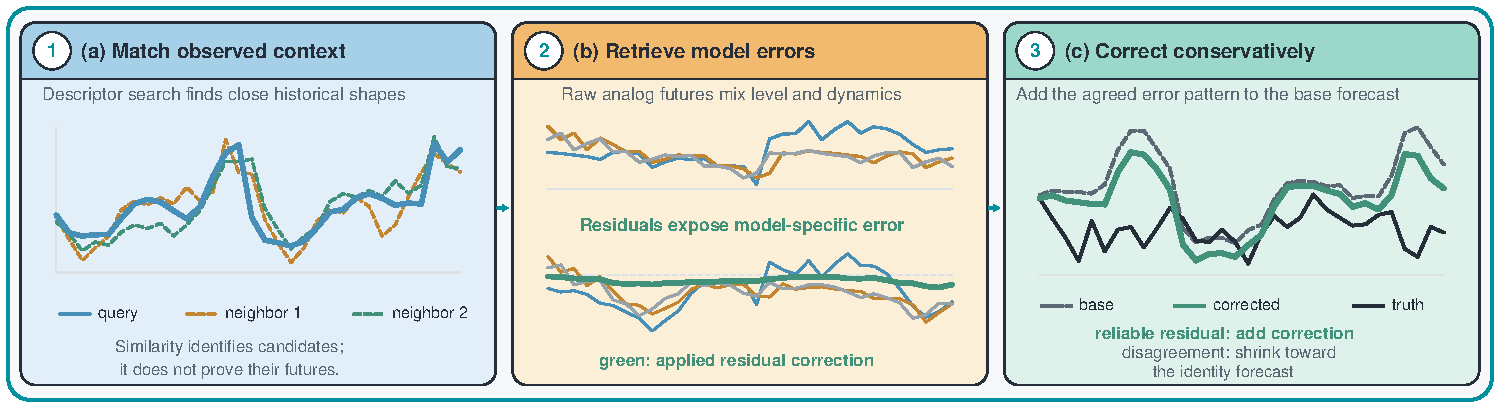
\includegraphics[width=\textwidth]{figures/residual_retrieval_example.pdf}
  \caption{\textbf{Residuals isolate model-specific error on real data.} An
  ETTh1 MULL example from a frozen TimeMixer. (a) Descriptor search returns
  historical windows with closely matching shapes. (b) Their raw futures sit at
  different levels and mix dynamics the base forecast already captures, whereas
  their residuals agree on a common error pattern. (c) Adding the shrunk
  residual moves the forecast toward the truth without disturbing its level.
  Panels (b)--(c) show a 36-step excerpt in the model's standardized space.}
  \label{fig:residual-example}
\end{figure*}

\begin{figure*}[t]
\hrule\vspace{2pt}
\textbf{Algorithm 1:} \method{} calibration and forecast-time revision\\[1pt]
\hrule\vspace{3pt}
\textbf{Input:} frozen forecaster $f$; validation stream
$\{(\xctx_i,\ytrue_i)\}$; candidate families and grids; metric set
$\mathcal{Q}$.\\
\textbf{Calibration.}
(1) For every validation origin $i$, evaluate $\ybase_i=f(\xctx_i)$ and, once
$\ytrue_i$ has fully elapsed, store
$(\feat_i,\ybase_i,\resid_i=\ytrue_i-\ybase_i)$ in $\mathcal{M}$.
(2) Split $\mathcal{M}$ chronologically into a memory prefix and a query
suffix.
(3) For each candidate $c$, form $\ycorr^{(c)}$ on the query suffix using only
the memory prefix and score it by $S(c)$.
(4) Lock the minimizing family and parameters $c^\star$; ties go to identity.\\
\textbf{Forecasting at origin $t$.}
(5) Evaluate $\ybase_t=f(\xctx_t)$ and build $\feat_t$ from $\xctx_t$ and
$\ybase_t$.
(6) If $c^\star$ is retrieval, take the top-$k$ items of $\mathcal{M}_t$ with
$i+H<t$, aggregate by Equation~\ref{eq:weights} and shrink by
Equation~\ref{eq:shrinkage}; otherwise evaluate the locked simpler correction.
(7) Return $\ycorr_t=\ybase_t+c_t$, leaving $f$ unchanged.\\
\vspace{1pt}\hrule
\end{figure*}

The ETTh1 example in Figure~\ref{fig:residual-example} was screened
deterministically for visualization only; the screening criteria and score
weights are recorded in the released case artifact and never enter method
selection.

\begin{table*}[h]
\centering
\small
\caption{Validation-only candidate space for the broad selector.}
\label{tab:search-space}
\begin{tabular}{p{0.22\textwidth}p{0.65\textwidth}}
\toprule
Family & Candidate values\\
\midrule
Identity & No parameters\\
Residual descriptor & Tail $\ell\in\{\min(48,L),L\}$; pooled steps
$\min(12,\ell)$; differences on; base forecast on/off; calendar on except PEMS;
at most 16 pooled channels\\
Residual aggregation &
$(k,\tau,\lambda)\in\{(8,0.1,1),(16,0.3,4)\}$;
$\alpha\in\{.05,.1,.2,.3,.5\}$\\
Seasonal blend & Long-term periods $\{4,8,12,24,48,96,168\}$, PEMS periods
$\{12,24,48,96\}$, and EPF periods $\{24,48,168\}$, each clipped at $L$ and
deduplicated; $\alpha\in\{.02,.05,.1,.2,.3\}$\\
Overlap blend & $(a,\gamma)\in\{(8,.75),(24,.9)\}$;
$\alpha\in\{.1,.25,.5\}$\\
Static residual bias & $\alpha\in\{.1,.25,.5,1\}$\\
Causal rolling bias & Window $W\in\{2H,8H,32H\}$; horizon block
$b\in\{0,\min(24,H)\}$; $\alpha\in\{.1,.25,.5,1\}$\\
\bottomrule
\end{tabular}
\end{table*}

\begin{table*}[h]
\centering
\small
\setlength{\tabcolsep}{5pt}
\caption{Information available to each correction candidate at forecast
origin $t$. A label is eligible only after its target timestamp has passed.}
\label{tab:candidate-availability}
\begin{tabular}{p{0.22\textwidth}p{0.68\textwidth}}
\toprule
Candidate & Information used\\
\midrule
Identity & Current frozen-model prediction only; no labels\\
Seasonal blend & Observed context through $t$; no labels\\
Overlap blend & Predictions issued at earlier origins for the same target
timestamps; no labels\\
Static residual bias & Validation predictions and validation labels\\
Historical residual retrieval & Validation contexts, predictions, and labels\\
Causal rolling bias & Validation evidence and test labels with target time
$u<t$\\
ETTm post-test retrieval & Validation evidence and completed official-test
residuals; no post-test label with target time $u\ge t$\\
ETTh online stack & Training data for NLinear, earlier predictions of the same
targets, and delayed labels with target time $u<t$\\
\bottomrule
\end{tabular}
\end{table*}

\paragraph{Temporal-candidate parameters.}
For overlap blend, $a$ is the maximum age in forecast origins and $\gamma$ is
the per-origin exponential decay. For causal rolling bias, $W$ is the
target-time lookback. Setting $b=0$ pools all forecast leads; otherwise,
contiguous groups of $b$ leads receive separate bias estimates. The grouping
changes which completed errors are averaged, not when a label becomes
eligible.

\paragraph{Chronological validation partition.}
Let validation contain $n$ forecast windows. The query suffix begins at
$\max(\lfloor n/2\rfloor,H+8)$, adjusted to stay below $n$. The residual
memory ends at least $H$ origins earlier, so every memory future is complete.
The final test retriever is fit on the complete validation split because that
split precedes test.

\paragraph{Selection tie breaking.}
Candidates minimize the worst-metric validation ratio $S(c)$ of
Section~\ref{sec:selection}. Identity wins an exact
score tie. When the best score is at least 0.982, only candidates improving
all validation metrics are eligible for family-prior selection. Within a
family, the lowest score wins; the family order is overlap, seasonal,
historical residual, static residual bias, and causal rolling bias.

\paragraph{Internal policy holdout.}
The supplementary material lists the fixed 123 development and 462 holdout
cell IDs. Membership uses the first 123 completed cells ordered by
\texttt{started\_unix} and does not use any metric value. The boundary is
nevertheless an opportunistic execution-order split rather than a stratified
dataset, model, or difficulty holdout. Its scope and balance diagnostics are
reported in Appendix~\ref{app:aggregate-results}.

\clearpage
\section{No-lookahead protocol}
\label{app:causality}

Every forecast and residual is associated with both an origin and its target
timestamps. Static validation memory is legal for test because all validation
targets precede test. Within online evaluation, a contribution for target
timestamp $u$ becomes visible only for query origin $t>u$. Prefix arrays are
queried at $t$, never $t+H$. Rolling-bias statistics write each residual
component at its own target timestamp and query the strict prefix $u<t$;
horizon blocks group forecast leads but cannot expose a partially realized
future.

The evaluation enforces four conditions:
\begin{enumerate}
  \item each retrieved residual's final target is earlier than the query
  origin;
  \item online statistics and weights contain only target-time evidence
  $u<t$, including when forecast windows overlap;
  \item the PEMS timeline includes the fresh-context gap and 12-step test
  stride; and
  \item post-test ETT memory may contain completed validation and
  official-test residuals but no current or future post-test target.
\end{enumerate}

Table~\ref{tab:candidate-availability} states the corresponding information
set for every candidate. Historical retrieval and static bias use validation
labels; seasonal and overlap corrections use no labels; causal rolling bias
may incorporate test-period labels only after their target timestamps have
passed. Thus the broad selector contains both static and delayed-label
prequential candidates.

As a direct no-lookahead check, we replace every label at timestamps
$\ge t$ and require the correction at $t$ to remain unchanged.

\clearpage
\section{Aggregate results}
\label{app:aggregate-results}

\begin{figure*}[t]
  \centering
  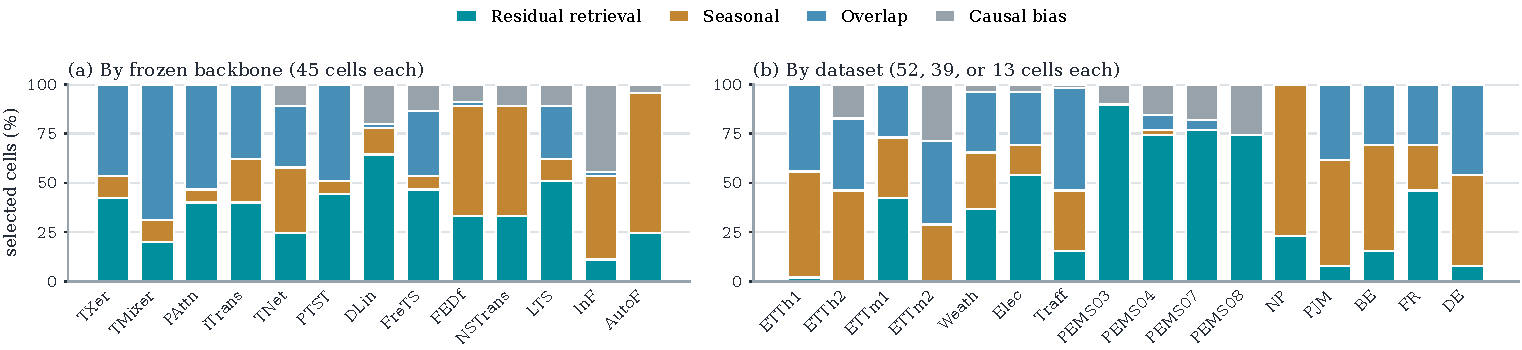
\includegraphics[width=\textwidth]{figures/selection_adaptivity.pdf}
  \caption{\textbf{Validation selects different corrections for different
  forecasters and regimes.} Share of the 585 primary settings in which each
  correction family was selected, grouped by frozen backbone (a) and by dataset
  (b). Error retrieval is chosen for 29/45 DLinear settings but 5/45 Informer
  settings, and for 35/39 PEMS03 settings but 0/52 ETTh2 settings. A fixed
  retrieval-always policy would be wrong in a large fraction of deployments.}
  \label{fig:selection}
\end{figure*}

\begin{table}[h]
\centering
\small
\caption{Primary A100 outcomes stratified by the correction family selected
on validation. This is descriptive attribution, not a
portfolio-minus-retrieval ablation.}
\label{tab:policy-attribution}
\begin{tabular}{lrr}
\toprule
Selected family & Cells & Strict wins\\
\midrule
Historical residual retrieval & 214 & 207\\
Seasonal blend & 156 & 151\\
Overlap blend & 159 & 148\\
Causal rolling bias & 56 & 56\\
Identity / static residual bias & 0 & 0\\
\midrule
Non-retrieval total & 371 & 355\\
\bottomrule
\end{tabular}
\end{table}

\begin{table*}[h]
\centering
\small
\caption{A100 configurations for the 214 cells that select historical
residual retrieval. Counts describe validation selections, not component
ablations. The search couples $(k,\tau,\lambda)$ into two settings.}
\label{tab:retrieval-configurations}
\begin{tabular}{lll}
\toprule
Quantity & Selected value & Cells\\
\midrule
Correction scale $\alpha$ & .05 / .1 / .2 / .3 / .5 & 0 / 1 / 6 / 29 / 178\\
Aggregation $(k,\tau,\lambda)$ & $(8,.1,1)$ / $(16,.3,4)$ & 151 / 63\\
Descriptor tail length & 48 / 96 / 168 & 57 / 148 / 9\\
Base-forecast features & Excluded / included & 61 / 153\\
\bottomrule
\end{tabular}
\end{table*}

All 214 selected retrieval configurations use first differences, 12 pooled
time steps, and a maximum of 16 channel groups; these fixed choices are not
ablated. Calendar features are present in 91 configurations and absent in 123,
the latter corresponding to PEMS where calendar marks are unavailable.

\begin{table*}[h]
\centering
\footnotesize
\setlength{\tabcolsep}{4pt}
\caption{A100 correction-family selections by dataset. HR is historical
residual retrieval, SB seasonal blend, OB overlap blend, and CB causal rolling
bias. Identity and static bias have zero selections on every dataset.}
\label{tab:dataset-policy-selection}
\begin{tabular}{lrrrrr@{\qquad}lrrrrr}
\toprule
Dataset & Cells & HR & SB & OB & CB &
Dataset & Cells & HR & SB & OB & CB\\
\midrule
ETTh1       & 52 & 1  & 28 & 23 & 0 &
ETTh2       & 52 & 0  & 24 & 19 & 9\\
ETTm1       & 52 & 22 & 16 & 14 & 0 &
ETTm2       & 52 & 0  & 15 & 22 & 15\\
Weather     & 52 & 19 & 15 & 16 & 2 &
Electricity & 52 & 28 & 8  & 14 & 2\\
Traffic     & 52 & 8  & 16 & 27 & 1 &
PEMS03      & 39 & 35 & 0  & 0  & 4\\
PEMS04      & 39 & 29 & 1  & 3  & 6 &
PEMS07      & 39 & 30 & 0  & 2  & 7\\
PEMS08      & 39 & 29 & 0  & 0  & 10 &
NP          & 13 & 3  & 10 & 0  & 0\\
PJM         & 13 & 1  & 7  & 5  & 0 &
BE          & 13 & 2  & 7  & 4  & 0\\
FR          & 13 & 6  & 3  & 4  & 0 &
DE          & 13 & 1  & 6  & 6  & 0\\
\bottomrule
\end{tabular}
\end{table*}

\begin{table*}[h]
\centering
\small
\setlength{\tabcolsep}{4pt}
\caption{The 23 A100 cells that do not strictly improve, grouped by dataset.
``Worst degradation'' is the largest percentage increase among reported test
metrics in that group. HR, SB, OB, and CB are defined in
Table~\ref{tab:dataset-policy-selection}.}
\label{tab:non-strict-cells}
\begin{tabular}{lrrrrrr}
\toprule
Dataset & Cells & HR & SB & OB & CB & Worst degradation\\
\midrule
Weather     & 7 & 6 & 0 & 1 & 0 & 2.45\%\\
DE          & 7 & 0 & 2 & 5 & 0 & 2.20\%\\
PEMS04      & 3 & 0 & 0 & 3 & 0 & 36.50\%\\
PEMS07      & 2 & 0 & 0 & 2 & 0 & 9.63\%\\
ETTh2       & 1 & 0 & 1 & 0 & 0 & 1.12\%\\
Electricity & 1 & 1 & 0 & 0 & 0 & 0.33\%\\
NP          & 1 & 0 & 1 & 0 & 0 & 2.64\%\\
BE          & 1 & 0 & 1 & 0 & 0 & 1.53\%\\
\midrule
Total       & 23 & 7 & 5 & 11 & 0 & 36.50\%\\
\bottomrule
\end{tabular}
\end{table*}

\begin{table}[h]
\centering
\small
\caption{A100--A10G discrepancy distribution over all 1,326 reported metric
values. Relative difference is absolute difference divided by the larger
absolute value. The frozen tolerance is
$10^{-5}+10^{-4}\max(|a|,|b|)$.}
\label{tab:hardware-consistency}
\begin{tabular}{lrr}
\toprule
Quantity & Baseline & Corrected\\
\midrule
Within tolerance & 472/1326 & 469/1326\\
Median relative difference & 0.09\% & 0.06\%\\
90th percentile & 2.95\% & 2.36\%\\
95th percentile & 5.80\% & 5.47\%\\
Maximum & 32.79\% & 28.13\%\\
\bottomrule
\end{tabular}
\end{table}

Selected methods agree in 569/585 cells, selected parameters in 529/585, and
strict-win classifications in 581/585. A100 remains the primary result; A10G
is a same-seed sensitivity check.

\section{Full benchmark decompositions}
\label{app:matrix-results}

The main tables average matched cells by dataset while accounting for the
fact that \method{} corrects each backbone independently.
Table~\ref{tab:long-term-horizons} and
Tables~\ref{tab:pems-horizons}--\ref{tab:pems-horizons-mape} expose every
dataset--horizon aggregate; each row contains exactly 13 paired backbone
cells. EPF has only horizon 24; its complete per-model view appears in the
full cell tables below.
Table~\ref{tab:backbone-results} instead aggregates by backbone and shows
strict wins together with paired relative reductions. The remaining tables in
this section report every one of the 585 primary cells. Each entry gives the
absolute error of the named backbone followed by the error after applying
\method{}; these tables do not average over backbones or horizons.

% Generated by paper/tools/generate_main_tables.py; do not edit.
\begin{table*}[p]
\centering
\scriptsize
\setlength{\tabcolsep}{3pt}
\caption{Full long-term results by prediction length. Absolute metrics average the same 13 paired backbones; $\Delta$ is the mean cell-wise relative reduction (\%).}
\label{tab:long-term-horizons}
\begin{tabular}{llrrrrrrr}
\toprule
Dataset & Horizon & Base MSE & +\method{} MSE & $\Delta$ MSE & Base MAE & +\method{} MAE & $\Delta$ MAE & Wins \\
\midrule
ETTh1 & 96 & 0.462 & \textbf{0.412} & 7.8 & 0.454 & \textbf{0.421} & 6.0 & 13/13 \\
ETTh1 & 192 & 0.499 & \textbf{0.457} & 5.7 & 0.478 & \textbf{0.451} & 4.5 & 13/13 \\
ETTh1 & 336 & 0.565 & \textbf{0.516} & 6.4 & 0.513 & \textbf{0.484} & 4.7 & 13/13 \\
ETTh1 & 720 & 0.607 & \textbf{0.544} & 7.3 & 0.553 & \textbf{0.522} & 4.5 & 13/13 \\
\midrule
ETTh2 & 96 & 0.452 & \textbf{0.322} & 12.8 & 0.437 & \textbf{0.368} & 9.8 & 13/13 \\
ETTh2 & 192 & 0.574 & \textbf{0.401} & 13.4 & 0.499 & \textbf{0.416} & 10.0 & 12/13 \\
ETTh2 & 336 & 0.634 & \textbf{0.446} & 14.9 & 0.540 & \textbf{0.450} & 10.7 & 13/13 \\
ETTh2 & 720 & 0.727 & \textbf{0.569} & 11.9 & 0.584 & \textbf{0.525} & 7.1 & 13/13 \\
\midrule
ETTm1 & 96 & 0.411 & \textbf{0.355} & 11.1 & 0.415 & \textbf{0.386} & 6.0 & 13/13 \\
ETTm1 & 192 & 0.455 & \textbf{0.403} & 8.8 & 0.437 & \textbf{0.409} & 5.5 & 13/13 \\
ETTm1 & 336 & 0.502 & \textbf{0.442} & 8.7 & 0.463 & \textbf{0.435} & 4.9 & 13/13 \\
ETTm1 & 720 & 0.571 & \textbf{0.502} & 9.4 & 0.501 & \textbf{0.471} & 4.8 & 13/13 \\
\midrule
ETTm2 & 96 & 0.241 & \textbf{0.193} & 10.1 & 0.310 & \textbf{0.279} & 6.8 & 13/13 \\
ETTm2 & 192 & 0.315 & \textbf{0.255} & 9.7 & 0.358 & \textbf{0.319} & 7.4 & 13/13 \\
ETTm2 & 336 & 0.417 & \textbf{0.317} & 13.4 & 0.417 & \textbf{0.357} & 9.8 & 13/13 \\
ETTm2 & 720 & 0.566 & \textbf{0.404} & 14.4 & 0.492 & \textbf{0.408} & 10.9 & 13/13 \\
\midrule
Weather & 96 & 0.223 & \textbf{0.194} & 8.9 & 0.271 & \textbf{0.250} & 5.6 & 13/13 \\
Weather & 192 & 0.271 & \textbf{0.243} & 6.8 & 0.309 & \textbf{0.291} & 4.1 & 9/13 \\
Weather & 336 & 0.348 & \textbf{0.287} & 8.4 & 0.356 & \textbf{0.320} & 5.9 & 10/13 \\
Weather & 720 & 0.435 & \textbf{0.358} & 7.6 & 0.410 & \textbf{0.367} & 5.7 & 13/13 \\
\midrule
Electricity & 96 & 0.243 & \textbf{0.197} & 9.7 & 0.326 & \textbf{0.294} & 6.4 & 13/13 \\
Electricity & 192 & 0.204 & \textbf{0.191} & 5.3 & 0.300 & \textbf{0.288} & 3.7 & 12/13 \\
Electricity & 336 & 0.219 & \textbf{0.205} & 5.8 & 0.316 & \textbf{0.302} & 4.1 & 13/13 \\
Electricity & 720 & 0.307 & \textbf{0.261} & 8.3 & 0.379 & \textbf{0.347} & 6.0 & 13/13 \\
\midrule
Traffic & 96 & 0.571 & \textbf{0.525} & 7.4 & 0.348 & \textbf{0.327} & 5.7 & 13/13 \\
Traffic & 192 & 0.579 & \textbf{0.537} & 6.4 & 0.353 & \textbf{0.332} & 5.5 & 13/13 \\
Traffic & 336 & 0.600 & \textbf{0.564} & 5.2 & 0.362 & \textbf{0.343} & 4.6 & 13/13 \\
Traffic & 720 & 0.642 & \textbf{0.608} & 4.5 & 0.382 & \textbf{0.366} & 3.8 & 13/13 \\
\bottomrule
\end{tabular}
\end{table*}

\clearpage
% Generated by paper/tools/generate_main_tables.py; do not edit.
\begin{table*}[p]
\centering
\footnotesize
\setlength{\tabcolsep}{6pt}
\caption{Full PEMS MAE results by prediction length. Absolute metrics average the same 13 paired backbones; $\Delta$ is the mean cell-wise relative reduction (\%). Strict wins require all three PEMS metrics and therefore repeat across these tables.}
\label{tab:pems-horizons}
\begin{tabular}{lrrrrr}
\toprule
Dataset & Horizon & Base MAE & +\method{} MAE & $\Delta$ MAE & Strict wins \\
\midrule
PEMS03 & 6 & 18.504 & \textbf{16.378} & 10.2 & 13/13 \\
PEMS03 & 12 & 20.037 & \textbf{17.545} & 11.6 & 13/13 \\
PEMS03 & 24 & 24.055 & \textbf{20.647} & 13.2 & 13/13 \\
\midrule
PEMS04 & 6 & 23.807 & \textbf{21.872} & 7.4 & 12/13 \\
PEMS04 & 12 & 26.688 & \textbf{23.728} & 9.5 & 12/13 \\
PEMS04 & 24 & 31.475 & \textbf{26.896} & 12.2 & 12/13 \\
\midrule
PEMS07 & 6 & 26.781 & \textbf{24.330} & 8.8 & 12/13 \\
PEMS07 & 12 & 29.145 & \textbf{25.604} & 11.3 & 12/13 \\
PEMS07 & 24 & 34.510 & \textbf{29.108} & 14.6 & 13/13 \\
\midrule
PEMS08 & 6 & 20.024 & \textbf{18.071} & 9.6 & 13/13 \\
PEMS08 & 12 & 22.363 & \textbf{19.316} & 12.6 & 13/13 \\
PEMS08 & 24 & 27.167 & \textbf{22.449} & 15.9 & 13/13 \\
\bottomrule
\end{tabular}
\end{table*}

\begin{table*}[p]
\centering
\footnotesize
\setlength{\tabcolsep}{6pt}
\caption{Full PEMS RMSE results by prediction length. Absolute metrics average the same 13 paired backbones; $\Delta$ is the mean cell-wise relative reduction (\%). Strict wins require all three PEMS metrics and therefore repeat across these tables.}
\label{tab:pems-horizons-rmse}
\begin{tabular}{lrrrrr}
\toprule
Dataset & Horizon & Base RMSE & +\method{} RMSE & $\Delta$ RMSE & Strict wins \\
\midrule
PEMS03 & 6 & 28.874 & \textbf{25.601} & 10.2 & 13/13 \\
PEMS03 & 12 & 31.319 & \textbf{27.566} & 11.3 & 13/13 \\
PEMS03 & 24 & 37.664 & \textbf{32.623} & 12.4 & 13/13 \\
\midrule
PEMS04 & 6 & 36.313 & \textbf{33.846} & 6.3 & 12/13 \\
PEMS04 & 12 & 40.393 & \textbf{36.414} & 8.7 & 12/13 \\
PEMS04 & 24 & 47.375 & \textbf{40.790} & 12.0 & 12/13 \\
\midrule
PEMS07 & 6 & 40.478 & \textbf{37.340} & 7.5 & 12/13 \\
PEMS07 & 12 & 44.220 & \textbf{39.634} & 9.7 & 12/13 \\
PEMS07 & 24 & 51.621 & \textbf{44.486} & 12.9 & 13/13 \\
\midrule
PEMS08 & 6 & 30.493 & \textbf{27.795} & 8.8 & 13/13 \\
PEMS08 & 12 & 33.811 & \textbf{29.497} & 11.9 & 13/13 \\
PEMS08 & 24 & 41.074 & \textbf{34.084} & 15.6 & 13/13 \\
\bottomrule
\end{tabular}
\end{table*}

\begin{table*}[p]
\centering
\footnotesize
\setlength{\tabcolsep}{6pt}
\caption{Full PEMS MAPE results by prediction length. Absolute metrics average the same 13 paired backbones; $\Delta$ is the mean cell-wise relative reduction (\%). Strict wins require all three PEMS metrics and therefore repeat across these tables.}
\label{tab:pems-horizons-mape}
\begin{tabular}{lrrrrr}
\toprule
Dataset & Horizon & Base MAPE & +\method{} MAPE & $\Delta$ MAPE & Strict wins \\
\midrule
PEMS03 & 6 & 0.187 & \textbf{0.164} & 10.5 & 13/13 \\
PEMS03 & 12 & 0.197 & \textbf{0.174} & 11.1 & 13/13 \\
PEMS03 & 24 & 0.238 & \textbf{0.207} & 12.4 & 13/13 \\
\midrule
PEMS04 & 6 & 0.166 & \textbf{0.147} & 10.2 & 12/13 \\
PEMS04 & 12 & 0.189 & \textbf{0.165} & 10.3 & 12/13 \\
PEMS04 & 24 & 0.221 & \textbf{0.188} & 11.8 & 12/13 \\
\midrule
PEMS07 & 6 & 0.122 & \textbf{0.107} & 11.8 & 12/13 \\
PEMS07 & 12 & 0.132 & \textbf{0.114} & 12.8 & 12/13 \\
PEMS07 & 24 & 0.165 & \textbf{0.135} & 16.2 & 13/13 \\
\midrule
PEMS08 & 6 & 0.125 & \textbf{0.111} & 10.2 & 13/13 \\
PEMS08 & 12 & 0.141 & \textbf{0.122} & 12.7 & 13/13 \\
PEMS08 & 24 & 0.174 & \textbf{0.147} & 14.5 & 13/13 \\
\bottomrule
\end{tabular}
\end{table*}

\clearpage
% Generated by paper/tools/generate_main_tables.py; do not edit.
\begin{table}[h!]
\centering
\footnotesize
\setlength{\tabcolsep}{2pt}
\caption{Backbone-level paired results. Entries are strict wins and mean cell-wise relative reductions (\%); positive values favor \method{}. This view prevents weak backbones or large absolute errors from dominating the conclusion.}
\label{tab:backbone-results}
\begin{tabular}{lrrr|rrrr|rrr}
\toprule
 & \multicolumn{3}{c|}{Long-term (28 cells)} & \multicolumn{4}{c|}{PEMS (12 cells)} & \multicolumn{3}{c}{EPF (5 cells)} \\
\cmidrule(lr){2-4} \cmidrule(lr){5-8} \cmidrule(lr){9-11}
Backbone & Wins & MSE & MAE & Wins & MAE & RMSE & MAPE & Wins & MSE & MAE \\
\midrule
\timexer{} & 28/28 & 1.1 & 0.9 & 12/12 & 14.1 & 11.9 & 15.9 & 3/5 & 0.3 & 0.4 \\
\timemixer{} & 27/28 & 1.3 & 1.2 & 7/12 & -2.4 & -0.8 & -5.5 & 4/5 & 3.2 & 2.5 \\
\pattn{} & 27/28 & 1.7 & 1.0 & 12/12 & 13.0 & 12.5 & 11.8 & 4/5 & 1.5 & 1.8 \\
\itransformer{} & 26/28 & 2.9 & 2.0 & 12/12 & 10.3 & 9.8 & 10.6 & 4/5 & 1.1 & 0.9 \\
\timesnet{} & 28/28 & 2.9 & 2.0 & 12/12 & 5.8 & 4.8 & 7.1 & 4/5 & 4.8 & 3.2 \\
\patchtst{} & 27/28 & 1.8 & 1.2 & 12/12 & 16.8 & 15.2 & 16.9 & 5/5 & 1.9 & 1.9 \\
\dlinear{} & 27/28 & 10.1 & 7.6 & 12/12 & 24.7 & 23.4 & 27.4 & 5/5 & 4.7 & 4.7 \\
\frets{} & 25/28 & 6.3 & 4.6 & 12/12 & 11.9 & 11.0 & 11.7 & 4/5 & 3.2 & 3.2 \\
\fedformer{} & 28/28 & 8.5 & 6.1 & 12/12 & 14.0 & 11.4 & 17.3 & 5/5 & 11.9 & 9.3 \\
\nonstatshort{} & 28/28 & 16.4 & 10.0 & 12/12 & 4.9 & 3.9 & 6.5 & 4/5 & 15.0 & 15.3 \\
\lightts{} & 28/28 & 10.3 & 7.8 & 12/12 & 9.4 & 8.2 & 9.0 & 4/5 & 1.6 & 2.2 \\
\informer{} & 28/28 & 41.3 & 28.7 & 12/12 & 8.4 & 9.7 & 10.2 & 5/5 & 9.7 & 6.1 \\
\autoformer{} & 28/28 & 11.6 & 8.0 & 12/12 & 17.4 & 17.0 & 17.4 & 5/5 & 17.5 & 10.7 \\
\bottomrule
\end{tabular}
\end{table}

\clearpage
% Generated by paper/tools/generate_main_tables.py; do not edit.
% Every accepted primary-matrix cell appears exactly once below.
\begin{table*}[p]
\centering
\scriptsize
\setlength{\tabcolsep}{3pt}
\caption{Complete long-term results on ETTh1. Base and +\method{} are reported separately for every backbone and horizon; bold marks a lower corrected error. No result in this table is averaged over backbones or horizons.}
\label{tab:full-long-term-etth1}
\begin{tabular}{llrrrrrrrr}
\toprule
Backbone & System & \multicolumn{2}{c}{96} & \multicolumn{2}{c}{192} & \multicolumn{2}{c}{336} & \multicolumn{2}{c}{720} \\
\cmidrule(lr){3-4} \cmidrule(lr){5-6} \cmidrule(lr){7-8} \cmidrule(lr){9-10}
 & & MSE & MAE & MSE & MAE & MSE & MAE & MSE & MAE \\
\midrule
TimeXer & Base & 0.3818 & 0.4029 & 0.4285 & 0.4355 & 0.4672 & 0.4494 & 0.4988 & 0.4926 \\
 & +\method{} & \textbf{0.3739} & \textbf{0.3932} & \textbf{0.4267} & \textbf{0.4342} & \textbf{0.4622} & \textbf{0.4457} & \textbf{0.4893} & \textbf{0.4871} \\
\addlinespace[1pt]
TimeMixer & Base & 0.3784 & 0.3981 & 0.4410 & 0.4301 & 0.5003 & 0.4600 & 0.4787 & 0.4724 \\
 & +\method{} & \textbf{0.3782} & \textbf{0.3895} & \textbf{0.4378} & \textbf{0.4278} & \textbf{0.4959} & \textbf{0.4568} & \textbf{0.4696} & \textbf{0.4680} \\
\addlinespace[1pt]
PAttn & Base & 0.3901 & 0.4048 & 0.4371 & 0.4392 & 0.4977 & 0.4703 & 0.5326 & 0.4995 \\
 & +\method{} & \textbf{0.3828} & \textbf{0.3961} & \textbf{0.4346} & \textbf{0.4374} & \textbf{0.4915} & \textbf{0.4662} & \textbf{0.5195} & \textbf{0.4927} \\
\addlinespace[1pt]
iTransformer & Base & 0.4469 & 0.4439 & 0.5187 & 0.4833 & 0.5538 & 0.5018 & 0.5629 & 0.5251 \\
 & +\method{} & \textbf{0.4054} & \textbf{0.4139} & \textbf{0.4679} & \textbf{0.4506} & \textbf{0.5107} & \textbf{0.4727} & \textbf{0.5124} & \textbf{0.4930} \\
\addlinespace[1pt]
TimesNet & Base & 0.3890 & 0.4120 & 0.4395 & 0.4418 & 0.4941 & 0.4709 & 0.5178 & 0.4944 \\
 & +\method{} & \textbf{0.3750} & \textbf{0.3933} & \textbf{0.4314} & \textbf{0.4258} & \textbf{0.4798} & \textbf{0.4519} & \textbf{0.5136} & \textbf{0.4928} \\
\addlinespace[1pt]
PatchTST & Base & 0.3793 & 0.3996 & 0.4274 & 0.4325 & 0.4783 & 0.4643 & 0.5220 & 0.5063 \\
 & +\method{} & \textbf{0.3727} & \textbf{0.3916} & \textbf{0.4266} & \textbf{0.4318} & \textbf{0.4736} & \textbf{0.4613} & \textbf{0.5121} & \textbf{0.5016} \\
\addlinespace[1pt]
DLinear & Base & 0.3962 & 0.4108 & 0.4450 & 0.4404 & 0.4874 & 0.4654 & 0.5126 & 0.5104 \\
 & +\method{} & \textbf{0.3861} & \textbf{0.3990} & \textbf{0.4441} & \textbf{0.4394} & \textbf{0.4776} & \textbf{0.4608} & \textbf{0.5114} & \textbf{0.5099} \\
\addlinespace[1pt]
FreTS & Base & 0.3999 & 0.4124 & 0.4512 & 0.4426 & 0.5086 & 0.4814 & 0.5627 & 0.5398 \\
 & +\method{} & \textbf{0.3928} & \textbf{0.4063} & \textbf{0.4436} & \textbf{0.4364} & \textbf{0.5000} & \textbf{0.4748} & \textbf{0.5497} & \textbf{0.5324} \\
\addlinespace[1pt]
FEDformer & Base & 0.3770 & 0.4184 & 0.4200 & 0.4441 & 0.4584 & 0.4666 & 0.5021 & 0.5032 \\
 & +\method{} & \textbf{0.3643} & \textbf{0.3945} & \textbf{0.4133} & \textbf{0.4239} & \textbf{0.4526} & \textbf{0.4515} & \textbf{0.4974} & \textbf{0.5008} \\
\addlinespace[1pt]
Non-stat. Transformer & Base & 0.5752 & 0.4933 & 0.4762 & 0.4783 & 0.7532 & 0.6289 & 0.8274 & 0.6659 \\
 & +\method{} & \textbf{0.4516} & \textbf{0.4353} & \textbf{0.4336} & \textbf{0.4411} & \textbf{0.6365} & \textbf{0.5645} & \textbf{0.6365} & \textbf{0.5716} \\
\addlinespace[1pt]
LightTS & Base & 0.4352 & 0.4436 & 0.4936 & 0.4782 & 0.5493 & 0.5103 & 0.6117 & 0.5688 \\
 & +\method{} & \textbf{0.4133} & \textbf{0.4280} & \textbf{0.4653} & \textbf{0.4592} & \textbf{0.5169} & \textbf{0.4900} & \textbf{0.5748} & \textbf{0.5492} \\
\addlinespace[1pt]
Informer & Base & 0.9590 & 0.7778 & 1.0199 & 0.7930 & 1.0310 & 0.7809 & 1.2219 & 0.8817 \\
 & +\method{} & \textbf{0.6328} & \textbf{0.6056} & \textbf{0.6812} & \textbf{0.6191} & \textbf{0.7092} & \textbf{0.6221} & \textbf{0.8044} & \textbf{0.6969} \\
\addlinespace[1pt]
Autoformer & Base & 0.4993 & 0.4807 & 0.4868 & 0.4756 & 0.5648 & 0.5242 & 0.5426 & 0.5231 \\
 & +\method{} & \textbf{0.4262} & \textbf{0.4328} & \textbf{0.4408} & \textbf{0.4400} & \textbf{0.5024} & \textbf{0.4801} & \textbf{0.4850} & \textbf{0.4849} \\
\bottomrule
\end{tabular}
\end{table*}

\begin{table*}[p]
\centering
\scriptsize
\setlength{\tabcolsep}{3pt}
\caption{Complete long-term results on ETTh2. Base and +\method{} are reported separately for every backbone and horizon; bold marks a lower corrected error. No result in this table is averaged over backbones or horizons.}
\label{tab:full-long-term-etth2}
\begin{tabular}{llrrrrrrrr}
\toprule
Backbone & System & \multicolumn{2}{c}{96} & \multicolumn{2}{c}{192} & \multicolumn{2}{c}{336} & \multicolumn{2}{c}{720} \\
\cmidrule(lr){3-4} \cmidrule(lr){5-6} \cmidrule(lr){7-8} \cmidrule(lr){9-10}
 & & MSE & MAE & MSE & MAE & MSE & MAE & MSE & MAE \\
\midrule
TimeXer & Base & 0.2854 & 0.3376 & 0.3627 & 0.3892 & 0.4113 & 0.4214 & 0.4485 & 0.4534 \\
 & +\method{} & \textbf{0.2842} & \textbf{0.3365} & \textbf{0.3606} & \textbf{0.3875} & \textbf{0.4076} & \textbf{0.4192} & \textbf{0.4481} & \textbf{0.4531} \\
\addlinespace[1pt]
TimeMixer & Base & 0.2878 & 0.3395 & 0.3778 & 0.3957 & 0.4247 & 0.4298 & 0.4681 & 0.4683 \\
 & +\method{} & \textbf{0.2875} & \textbf{0.3391} & 0.3820 & \textbf{0.3917} & \textbf{0.4163} & \textbf{0.4246} & \textbf{0.4671} & \textbf{0.4674} \\
\addlinespace[1pt]
PAttn & Base & 0.2988 & 0.3453 & 0.3826 & 0.3954 & 0.4232 & 0.4305 & 0.4279 & 0.4438 \\
 & +\method{} & \textbf{0.2941} & \textbf{0.3408} & \textbf{0.3782} & \textbf{0.3917} & \textbf{0.4182} & \textbf{0.4269} & \textbf{0.4233} & \textbf{0.4407} \\
\addlinespace[1pt]
iTransformer & Base & 0.3004 & 0.3496 & 0.3818 & 0.3998 & 0.4236 & 0.4324 & 0.4264 & 0.4451 \\
 & +\method{} & \textbf{0.2997} & \textbf{0.3435} & \textbf{0.3787} & \textbf{0.3969} & \textbf{0.4202} & \textbf{0.4298} & \textbf{0.4231} & \textbf{0.4426} \\
\addlinespace[1pt]
TimesNet & Base & 0.3370 & 0.3709 & 0.4046 & 0.4146 & 0.4520 & 0.4503 & 0.4337 & 0.4477 \\
 & +\method{} & \textbf{0.3140} & \textbf{0.3536} & \textbf{0.3896} & \textbf{0.4015} & \textbf{0.4340} & \textbf{0.4357} & \textbf{0.4305} & \textbf{0.4455} \\
\addlinespace[1pt]
PatchTST & Base & 0.2921 & 0.3452 & 0.3814 & 0.4044 & 0.4185 & 0.4349 & 0.4332 & 0.4524 \\
 & +\method{} & \textbf{0.2890} & \textbf{0.3421} & \textbf{0.3752} & \textbf{0.4006} & \textbf{0.4103} & \textbf{0.4306} & \textbf{0.4298} & \textbf{0.4502} \\
\addlinespace[1pt]
DLinear & Base & 0.3414 & 0.3953 & 0.4819 & 0.4792 & 0.5929 & 0.5422 & 0.8403 & 0.6611 \\
 & +\method{} & \textbf{0.2996} & \textbf{0.3483} & \textbf{0.3584} & \textbf{0.3902} & \textbf{0.4123} & \textbf{0.4255} & \textbf{0.6150} & \textbf{0.5612} \\
\addlinespace[1pt]
FreTS & Base & 0.3415 & 0.3967 & 0.4396 & 0.4492 & 0.5375 & 0.5094 & 0.7956 & 0.6436 \\
 & +\method{} & \textbf{0.3013} & \textbf{0.3538} & \textbf{0.4045} & \textbf{0.4207} & \textbf{0.4720} & \textbf{0.4707} & \textbf{0.5933} & \textbf{0.5511} \\
\addlinespace[1pt]
FEDformer & Base & 0.3480 & 0.3906 & 0.4245 & 0.4371 & 0.4566 & 0.4676 & 0.4758 & 0.4858 \\
 & +\method{} & \textbf{0.3190} & \textbf{0.3653} & \textbf{0.3994} & \textbf{0.4133} & \textbf{0.4388} & \textbf{0.4481} & \textbf{0.4502} & \textbf{0.4638} \\
\addlinespace[1pt]
Non-stat. Transformer & Base & 0.4594 & 0.4509 & 0.6137 & 0.5253 & 0.7591 & 0.5913 & 0.5136 & 0.4918 \\
 & +\method{} & \textbf{0.3688} & \textbf{0.3963} & \textbf{0.4933} & \textbf{0.4618} & \textbf{0.5975} & \textbf{0.5148} & \textbf{0.4538} & \textbf{0.4586} \\
\addlinespace[1pt]
LightTS & Base & 0.4353 & 0.4730 & 0.5613 & 0.5382 & 0.6829 & 0.5985 & 0.9366 & 0.7145 \\
 & +\method{} & \textbf{0.3615} & \textbf{0.4144} & \textbf{0.4604} & \textbf{0.4708} & \textbf{0.4795} & \textbf{0.4857} & \textbf{0.6603} & \textbf{0.5912} \\
\addlinespace[1pt]
Informer & Base & 1.7643 & 1.0737 & 2.2024 & 1.2022 & 2.1738 & 1.2303 & 2.7496 & 1.3864 \\
 & +\method{} & \textbf{0.4310} & \textbf{0.4645} & \textbf{0.4212} & \textbf{0.4602} & \textbf{0.4386} & \textbf{0.4705} & \textbf{1.5481} & \textbf{1.0228} \\
\addlinespace[1pt]
Autoformer & Base & 0.3817 & 0.4150 & 0.4512 & 0.4530 & 0.4833 & 0.4830 & 0.5035 & 0.5025 \\
 & +\method{} & \textbf{0.3363} & \textbf{0.3848} & \textbf{0.4106} & \textbf{0.4257} & \textbf{0.4567} & \textbf{0.4620} & \textbf{0.4599} & \textbf{0.4732} \\
\bottomrule
\end{tabular}
\end{table*}

\begin{table*}[p]
\centering
\scriptsize
\setlength{\tabcolsep}{3pt}
\caption{Complete long-term results on ETTm1. Base and +\method{} are reported separately for every backbone and horizon; bold marks a lower corrected error. No result in this table is averaged over backbones or horizons.}
\label{tab:full-long-term-ettm1}
\begin{tabular}{llrrrrrrrr}
\toprule
Backbone & System & \multicolumn{2}{c}{96} & \multicolumn{2}{c}{192} & \multicolumn{2}{c}{336} & \multicolumn{2}{c}{720} \\
\cmidrule(lr){3-4} \cmidrule(lr){5-6} \cmidrule(lr){7-8} \cmidrule(lr){9-10}
 & & MSE & MAE & MSE & MAE & MSE & MAE & MSE & MAE \\
\midrule
TimeXer & Base & 0.3178 & 0.3563 & 0.3616 & 0.3829 & 0.3951 & 0.4067 & 0.4524 & 0.4413 \\
 & +\method{} & \textbf{0.3072} & \textbf{0.3514} & \textbf{0.3583} & \textbf{0.3808} & \textbf{0.3872} & \textbf{0.4020} & \textbf{0.4470} & \textbf{0.4401} \\
\addlinespace[1pt]
TimeMixer & Base & 0.3184 & 0.3581 & 0.3654 & 0.3868 & 0.3894 & 0.4027 & 0.4697 & 0.4528 \\
 & +\method{} & \textbf{0.3040} & \textbf{0.3515} & \textbf{0.3560} & \textbf{0.3805} & \textbf{0.3812} & \textbf{0.3974} & \textbf{0.4515} & \textbf{0.4453} \\
\addlinespace[1pt]
PAttn & Base & 0.3364 & 0.3648 & 0.3762 & 0.3832 & 0.4074 & 0.4036 & 0.4674 & 0.4376 \\
 & +\method{} & \textbf{0.3201} & \textbf{0.3583} & \textbf{0.3737} & \textbf{0.3808} & \textbf{0.4048} & \textbf{0.4012} & \textbf{0.4533} & \textbf{0.4357} \\
\addlinespace[1pt]
iTransformer & Base & 0.3557 & 0.3813 & 0.3988 & 0.4020 & 0.4330 & 0.4242 & 0.5005 & 0.4615 \\
 & +\method{} & \textbf{0.3379} & \textbf{0.3733} & \textbf{0.3973} & \textbf{0.4007} & \textbf{0.4315} & \textbf{0.4231} & \textbf{0.4800} & \textbf{0.4582} \\
\addlinespace[1pt]
TimesNet & Base & 0.3339 & 0.3754 & 0.4081 & 0.4137 & 0.4150 & 0.4223 & 0.5101 & 0.4722 \\
 & +\method{} & \textbf{0.3180} & \textbf{0.3602} & \textbf{0.3771} & \textbf{0.3878} & \textbf{0.4134} & \textbf{0.4212} & \textbf{0.5034} & \textbf{0.4704} \\
\addlinespace[1pt]
PatchTST & Base & 0.3268 & 0.3664 & 0.3700 & 0.3903 & 0.3982 & 0.4084 & 0.4577 & 0.4444 \\
 & +\method{} & \textbf{0.3131} & \textbf{0.3602} & \textbf{0.3668} & \textbf{0.3883} & \textbf{0.3956} & \textbf{0.4066} & \textbf{0.4484} & \textbf{0.4412} \\
\addlinespace[1pt]
DLinear & Base & 0.3459 & 0.3737 & 0.3818 & 0.3911 & 0.4153 & 0.4150 & 0.4730 & 0.4509 \\
 & +\method{} & \textbf{0.3205} & \textbf{0.3620} & \textbf{0.3807} & \textbf{0.3898} & \textbf{0.4078} & \textbf{0.4118} & \textbf{0.4557} & \textbf{0.4455} \\
\addlinespace[1pt]
FreTS & Base & 0.3398 & 0.3754 & 0.3833 & 0.3984 & 0.4202 & 0.4250 & 0.4975 & 0.4742 \\
 & +\method{} & \textbf{0.3247} & \textbf{0.3663} & \textbf{0.3787} & \textbf{0.3949} & \textbf{0.4159} & \textbf{0.4218} & \textbf{0.4821} & \textbf{0.4670} \\
\addlinespace[1pt]
FEDformer & Base & 0.5353 & 0.4892 & 0.5273 & 0.4908 & 0.6801 & 0.5477 & 0.7092 & 0.5623 \\
 & +\method{} & \textbf{0.4252} & \textbf{0.4418} & \textbf{0.4238} & \textbf{0.4314} & \textbf{0.5074} & \textbf{0.4858} & \textbf{0.5556} & \textbf{0.5081} \\
\addlinespace[1pt]
Non-stat. Transformer & Base & 0.5062 & 0.4644 & 0.6041 & 0.4973 & 0.6640 & 0.5186 & 0.7208 & 0.5431 \\
 & +\method{} & \textbf{0.3945} & \textbf{0.4076} & \textbf{0.4652} & \textbf{0.4350} & \textbf{0.5083} & \textbf{0.4560} & \textbf{0.5741} & \textbf{0.4850} \\
\addlinespace[1pt]
LightTS & Base & 0.3691 & 0.3914 & 0.3994 & 0.4056 & 0.4296 & 0.4261 & 0.4876 & 0.4623 \\
 & +\method{} & \textbf{0.3384} & \textbf{0.3767} & \textbf{0.3796} & \textbf{0.3967} & \textbf{0.4243} & \textbf{0.4217} & \textbf{0.4682} & \textbf{0.4557} \\
\addlinespace[1pt]
Informer & Base & 0.7403 & 0.6205 & 0.7609 & 0.6270 & 0.8722 & 0.6878 & 0.9979 & 0.7377 \\
 & +\method{} & \textbf{0.5049} & \textbf{0.4937} & \textbf{0.5280} & \textbf{0.5034} & \textbf{0.5926} & \textbf{0.5453} & \textbf{0.6693} & \textbf{0.5802} \\
\addlinespace[1pt]
Autoformer & Base & 0.5198 & 0.4821 & 0.5781 & 0.5123 & 0.6100 & 0.5325 & 0.6812 & 0.5671 \\
 & +\method{} & \textbf{0.4015} & \textbf{0.4169} & \textbf{0.4486} & \textbf{0.4437} & \textbf{0.4743} & \textbf{0.4629} & \textbf{0.5340} & \textbf{0.4949} \\
\bottomrule
\end{tabular}
\end{table*}

\begin{table*}[p]
\centering
\scriptsize
\setlength{\tabcolsep}{3pt}
\caption{Complete long-term results on ETTm2. Base and +\method{} are reported separately for every backbone and horizon; bold marks a lower corrected error. No result in this table is averaged over backbones or horizons.}
\label{tab:full-long-term-ettm2}
\begin{tabular}{llrrrrrrrr}
\toprule
Backbone & System & \multicolumn{2}{c}{96} & \multicolumn{2}{c}{192} & \multicolumn{2}{c}{336} & \multicolumn{2}{c}{720} \\
\cmidrule(lr){3-4} \cmidrule(lr){5-6} \cmidrule(lr){7-8} \cmidrule(lr){9-10}
 & & MSE & MAE & MSE & MAE & MSE & MAE & MSE & MAE \\
\midrule
TimeXer & Base & 0.1712 & 0.2560 & 0.2365 & 0.2987 & 0.2953 & 0.3379 & 0.3934 & 0.3942 \\
 & +\method{} & \textbf{0.1707} & \textbf{0.2557} & \textbf{0.2358} & \textbf{0.2980} & \textbf{0.2926} & \textbf{0.3359} & \textbf{0.3908} & \textbf{0.3924} \\
\addlinespace[1pt]
TimeMixer & Base & 0.1750 & 0.2574 & 0.2360 & 0.2975 & 0.3026 & 0.3410 & 0.4009 & 0.4054 \\
 & +\method{} & \textbf{0.1743} & \textbf{0.2569} & \textbf{0.2350} & \textbf{0.2966} & \textbf{0.2994} & \textbf{0.3379} & \textbf{0.3958} & \textbf{0.4021} \\
\addlinespace[1pt]
PAttn & Base & 0.1800 & 0.2668 & 0.2462 & 0.3079 & 0.3084 & 0.3471 & 0.4076 & 0.4031 \\
 & +\method{} & \textbf{0.1788} & \textbf{0.2657} & \textbf{0.2448} & \textbf{0.3066} & \textbf{0.3057} & \textbf{0.3451} & \textbf{0.4045} & \textbf{0.4009} \\
\addlinespace[1pt]
iTransformer & Base & 0.1862 & 0.2723 & 0.2516 & 0.3119 & 0.3153 & 0.3527 & 0.4132 & 0.4060 \\
 & +\method{} & \textbf{0.1830} & \textbf{0.2658} & \textbf{0.2498} & \textbf{0.3095} & \textbf{0.3125} & \textbf{0.3499} & \textbf{0.4098} & \textbf{0.4031} \\
\addlinespace[1pt]
TimesNet & Base & 0.1894 & 0.2662 & 0.2634 & 0.3119 & 0.3204 & 0.3488 & 0.4229 & 0.4069 \\
 & +\method{} & \textbf{0.1807} & \textbf{0.2623} & \textbf{0.2630} & \textbf{0.3114} & \textbf{0.3195} & \textbf{0.3479} & \textbf{0.4208} & \textbf{0.4058} \\
\addlinespace[1pt]
PatchTST & Base & 0.1828 & 0.2679 & 0.2463 & 0.3058 & 0.3105 & 0.3492 & 0.4150 & 0.4108 \\
 & +\method{} & \textbf{0.1793} & \textbf{0.2654} & \textbf{0.2446} & \textbf{0.3045} & \textbf{0.3082} & \textbf{0.3478} & \textbf{0.4108} & \textbf{0.4083} \\
\addlinespace[1pt]
DLinear & Base & 0.1934 & 0.2928 & 0.2845 & 0.3614 & 0.3849 & 0.4295 & 0.5561 & 0.5235 \\
 & +\method{} & \textbf{0.1771} & \textbf{0.2639} & \textbf{0.2394} & \textbf{0.3033} & \textbf{0.2840} & \textbf{0.3357} & \textbf{0.3908} & \textbf{0.3993} \\
\addlinespace[1pt]
FreTS & Base & 0.1943 & 0.2846 & 0.2774 & 0.3507 & 0.3698 & 0.4042 & 0.5602 & 0.5186 \\
 & +\method{} & \textbf{0.1771} & \textbf{0.2656} & \textbf{0.2593} & \textbf{0.3280} & \textbf{0.2855} & \textbf{0.3384} & \textbf{0.3841} & \textbf{0.3997} \\
\addlinespace[1pt]
FEDformer & Base & 0.2098 & 0.2933 & 0.2710 & 0.3288 & 0.3275 & 0.3641 & 0.4204 & 0.4164 \\
 & +\method{} & \textbf{0.1949} & \textbf{0.2845} & \textbf{0.2578} & \textbf{0.3213} & \textbf{0.3186} & \textbf{0.3586} & \textbf{0.4136} & \textbf{0.4051} \\
\addlinespace[1pt]
Non-stat. Transformer & Base & 0.2233 & 0.3008 & 0.2680 & 0.3234 & 0.4862 & 0.4538 & 0.4572 & 0.4351 \\
 & +\method{} & \textbf{0.2029} & \textbf{0.2814} & \textbf{0.2478} & \textbf{0.3067} & \textbf{0.3899} & \textbf{0.3997} & \textbf{0.4260} & \textbf{0.4132} \\
\addlinespace[1pt]
LightTS & Base & 0.2088 & 0.3076 & 0.3005 & 0.3748 & 0.3933 & 0.4347 & 0.5449 & 0.5188 \\
 & +\method{} & \textbf{0.1934} & \textbf{0.2831} & \textbf{0.2510} & \textbf{0.3164} & \textbf{0.2983} & \textbf{0.3495} & \textbf{0.3755} & \textbf{0.3993} \\
\addlinespace[1pt]
Informer & Base & 0.7444 & 0.6312 & 0.9328 & 0.7436 & 1.2786 & 0.8891 & 1.9379 & 1.1306 \\
 & +\method{} & \textbf{0.2816} & \textbf{0.3771} & \textbf{0.3287} & \textbf{0.4149} & \textbf{0.3936} & \textbf{0.4399} & \textbf{0.4170} & \textbf{0.4590} \\
\addlinespace[1pt]
Autoformer & Base & 0.2719 & 0.3291 & 0.2845 & 0.3429 & 0.3319 & 0.3669 & 0.4277 & 0.4223 \\
 & +\method{} & \textbf{0.2212} & \textbf{0.3031} & \textbf{0.2624} & \textbf{0.3277} & \textbf{0.3173} & \textbf{0.3573} & \textbf{0.4162} & \textbf{0.4132} \\
\bottomrule
\end{tabular}
\end{table*}

\begin{table*}[p]
\centering
\scriptsize
\setlength{\tabcolsep}{3pt}
\caption{Complete long-term results on Weather. Base and +\method{} are reported separately for every backbone and horizon; bold marks a lower corrected error. No result in this table is averaged over backbones or horizons.}
\label{tab:full-long-term-weather}
\begin{tabular}{llrrrrrrrr}
\toprule
Backbone & System & \multicolumn{2}{c}{96} & \multicolumn{2}{c}{192} & \multicolumn{2}{c}{336} & \multicolumn{2}{c}{720} \\
\cmidrule(lr){3-4} \cmidrule(lr){5-6} \cmidrule(lr){7-8} \cmidrule(lr){9-10}
 & & MSE & MAE & MSE & MAE & MSE & MAE & MSE & MAE \\
\midrule
TimeXer & Base & 0.1786 & 0.2244 & 0.2041 & 0.2475 & 0.2607 & 0.2895 & 0.3400 & 0.3404 \\
 & +\method{} & \textbf{0.1746} & \textbf{0.2236} & \textbf{0.2034} & \textbf{0.2473} & \textbf{0.2598} & \textbf{0.2892} & \textbf{0.3388} & \textbf{0.3398} \\
\addlinespace[1pt]
TimeMixer & Base & 0.1610 & 0.2079 & 0.2064 & 0.2507 & 0.2635 & 0.2917 & 0.3438 & 0.3436 \\
 & +\method{} & \textbf{0.1606} & \textbf{0.2077} & \textbf{0.2057} & \textbf{0.2503} & \textbf{0.2630} & \textbf{0.2916} & \textbf{0.3423} & \textbf{0.3426} \\
\addlinespace[1pt]
PAttn & Base & 0.1894 & 0.2263 & 0.2341 & 0.2641 & 0.2873 & 0.3015 & 0.3622 & 0.3495 \\
 & +\method{} & \textbf{0.1837} & \textbf{0.2257} & \textbf{0.2328} & 0.2706 & \textbf{0.2862} & \textbf{0.3012} & \textbf{0.3602} & \textbf{0.3488} \\
\addlinespace[1pt]
iTransformer & Base & 0.1971 & 0.2366 & 0.2432 & 0.2738 & 0.2951 & 0.3104 & 0.3611 & 0.3510 \\
 & +\method{} & \textbf{0.1902} & \textbf{0.2340} & \textbf{0.2378} & 0.2745 & \textbf{0.2879} & 0.3105 & \textbf{0.3572} & \textbf{0.3490} \\
\addlinespace[1pt]
TimesNet & Base & 0.1690 & 0.2195 & 0.2247 & 0.2640 & 0.2815 & 0.3036 & 0.3566 & 0.3526 \\
 & +\method{} & \textbf{0.1658} & \textbf{0.2168} & \textbf{0.2245} & \textbf{0.2639} & \textbf{0.2811} & \textbf{0.3034} & \textbf{0.3554} & \textbf{0.3519} \\
\addlinespace[1pt]
PatchTST & Base & 0.1722 & 0.2135 & 0.2200 & 0.2556 & 0.2794 & 0.2979 & 0.3546 & 0.3467 \\
 & +\method{} & \textbf{0.1677} & \textbf{0.2129} & \textbf{0.2194} & 0.2556 & \textbf{0.2788} & \textbf{0.2978} & \textbf{0.3534} & \textbf{0.3462} \\
\addlinespace[1pt]
DLinear & Base & 0.1962 & 0.2561 & 0.2389 & 0.2992 & 0.2811 & 0.3306 & 0.3454 & 0.3819 \\
 & +\method{} & \textbf{0.1901} & \textbf{0.2506} & \textbf{0.2360} & \textbf{0.2987} & \textbf{0.2785} & 0.3308 & \textbf{0.3353} & \textbf{0.3759} \\
\addlinespace[1pt]
FreTS & Base & 0.1843 & 0.2386 & 0.2226 & 0.2735 & 0.2724 & 0.3175 & 0.3544 & 0.3868 \\
 & +\method{} & \textbf{0.1797} & \textbf{0.2355} & \textbf{0.2218} & 0.2771 & \textbf{0.2704} & 0.3198 & \textbf{0.3519} & \textbf{0.3857} \\
\addlinespace[1pt]
FEDformer & Base & 0.2713 & 0.3419 & 0.3217 & 0.3774 & 0.3282 & 0.3654 & 0.3938 & 0.3993 \\
 & +\method{} & \textbf{0.2038} & \textbf{0.2778} & \textbf{0.2603} & \textbf{0.3210} & \textbf{0.2997} & \textbf{0.3356} & \textbf{0.3817} & \textbf{0.3959} \\
\addlinespace[1pt]
Non-stat. Transformer & Base & 0.2086 & 0.2512 & 0.2787 & 0.3057 & 0.3649 & 0.3584 & 0.3928 & 0.3789 \\
 & +\method{} & \textbf{0.1836} & \textbf{0.2317} & \textbf{0.2394} & \textbf{0.2778} & \textbf{0.3159} & \textbf{0.3283} & \textbf{0.3707} & \textbf{0.3636} \\
\addlinespace[1pt]
LightTS & Base & 0.1964 & 0.2552 & 0.2419 & 0.2987 & 0.2899 & 0.3365 & 0.3497 & 0.3834 \\
 & +\method{} & \textbf{0.1904} & \textbf{0.2491} & \textbf{0.2392} & \textbf{0.2982} & \textbf{0.2822} & \textbf{0.3323} & \textbf{0.3384} & \textbf{0.3782} \\
\addlinespace[1pt]
Informer & Base & 0.5204 & 0.5156 & 0.5769 & 0.5391 & 0.9701 & 0.7332 & 1.2664 & 0.8835 \\
 & +\method{} & \textbf{0.3321} & \textbf{0.3994} & \textbf{0.3830} & \textbf{0.4274} & \textbf{0.3254} & \textbf{0.3776} & \textbf{0.3776} & \textbf{0.3929} \\
\addlinespace[1pt]
Autoformer & Base & 0.2582 & 0.3310 & 0.3039 & 0.3625 & 0.3481 & 0.3888 & 0.4332 & 0.4336 \\
 & +\method{} & \textbf{0.2056} & \textbf{0.2806} & \textbf{0.2575} & \textbf{0.3186} & \textbf{0.3021} & \textbf{0.3440} & \textbf{0.3907} & \textbf{0.3956} \\
\bottomrule
\end{tabular}
\end{table*}

\begin{table*}[p]
\centering
\scriptsize
\setlength{\tabcolsep}{3pt}
\caption{Complete long-term results on Electricity. Base and +\method{} are reported separately for every backbone and horizon; bold marks a lower corrected error. No result in this table is averaged over backbones or horizons.}
\label{tab:full-long-term-electricity}
\begin{tabular}{llrrrrrrrr}
\toprule
Backbone & System & \multicolumn{2}{c}{96} & \multicolumn{2}{c}{192} & \multicolumn{2}{c}{336} & \multicolumn{2}{c}{720} \\
\cmidrule(lr){3-4} \cmidrule(lr){5-6} \cmidrule(lr){7-8} \cmidrule(lr){9-10}
 & & MSE & MAE & MSE & MAE & MSE & MAE & MSE & MAE \\
\midrule
TimeXer & Base & 0.1405 & 0.2425 & 0.1571 & 0.2556 & 0.1769 & 0.2752 & 0.2110 & 0.3061 \\
 & +\method{} & \textbf{0.1400} & \textbf{0.2379} & \textbf{0.1564} & \textbf{0.2525} & \textbf{0.1739} & \textbf{0.2693} & \textbf{0.2055} & \textbf{0.3011} \\
\addlinespace[1pt]
TimeMixer & Base & 0.1562 & 0.2476 & 0.1701 & 0.2610 & 0.1868 & 0.2773 & 0.2283 & 0.3131 \\
 & +\method{} & \textbf{0.1528} & \textbf{0.2447} & \textbf{0.1679} & \textbf{0.2590} & \textbf{0.1841} & \textbf{0.2751} & \textbf{0.2251} & \textbf{0.3105} \\
\addlinespace[1pt]
PAttn & Base & 0.1846 & 0.2668 & 0.1887 & 0.2717 & 0.2043 & 0.2875 & 0.2467 & 0.3216 \\
 & +\method{} & \textbf{0.1737} & \textbf{0.2620} & \textbf{0.1865} & \textbf{0.2700} & \textbf{0.2014} & \textbf{0.2854} & \textbf{0.2436} & \textbf{0.3191} \\
\addlinespace[1pt]
iTransformer & Base & 0.1488 & 0.2406 & 0.1645 & 0.2560 & 0.1784 & 0.2712 & 0.2271 & 0.3114 \\
 & +\method{} & \textbf{0.1443} & \textbf{0.2364} & \textbf{0.1611} & \textbf{0.2528} & \textbf{0.1738} & \textbf{0.2670} & \textbf{0.2206} & \textbf{0.3050} \\
\addlinespace[1pt]
TimesNet & Base & 0.1679 & 0.2716 & 0.1860 & 0.2883 & 0.2036 & 0.3051 & 0.2203 & 0.3183 \\
 & +\method{} & \textbf{0.1649} & \textbf{0.2676} & \textbf{0.1739} & \textbf{0.2747} & \textbf{0.1961} & \textbf{0.2948} & \textbf{0.2166} & \textbf{0.3156} \\
\addlinespace[1pt]
PatchTST & Base & 0.1800 & 0.2730 & 0.1874 & 0.2797 & 0.2043 & 0.2960 & 0.2455 & 0.3283 \\
 & +\method{} & \textbf{0.1697} & \textbf{0.2622} & \textbf{0.1835} & \textbf{0.2743} & \textbf{0.1949} & \textbf{0.2856} & \textbf{0.2431} & \textbf{0.3267} \\
\addlinespace[1pt]
DLinear & Base & 0.2104 & 0.3016 & 0.2102 & 0.3047 & 0.2231 & 0.3192 & 0.2578 & 0.3496 \\
 & +\method{} & \textbf{0.1897} & \textbf{0.2848} & \textbf{0.2007} & \textbf{0.2950} & \textbf{0.2058} & \textbf{0.3022} & \textbf{0.2551} & \textbf{0.3424} \\
\addlinespace[1pt]
FreTS & Base & 0.1895 & 0.2768 & 0.1917 & 0.2792 & 0.2069 & 0.2966 & 0.2467 & 0.3333 \\
 & +\method{} & \textbf{0.1782} & \textbf{0.2704} & \textbf{0.1900} & 0.2801 & \textbf{0.1987} & \textbf{0.2897} & \textbf{0.2427} & \textbf{0.3270} \\
\addlinespace[1pt]
FEDformer & Base & 0.1948 & 0.3089 & 0.2022 & 0.3155 & 0.2292 & 0.3423 & 0.2620 & 0.3655 \\
 & +\method{} & \textbf{0.1831} & \textbf{0.2945} & \textbf{0.1905} & \textbf{0.3001} & \textbf{0.2071} & \textbf{0.3188} & \textbf{0.2420} & \textbf{0.3377} \\
\addlinespace[1pt]
Non-stat. Transformer & Base & 0.8414 & 0.7579 & 0.1836 & 0.2857 & 0.2002 & 0.3033 & 0.8928 & 0.7727 \\
 & +\method{} & \textbf{0.4065} & \textbf{0.4973} & \textbf{0.1705} & \textbf{0.2684} & \textbf{0.1867} & \textbf{0.2887} & \textbf{0.4818} & \textbf{0.5314} \\
\addlinespace[1pt]
LightTS & Base & 0.2133 & 0.3156 & 0.2218 & 0.3251 & 0.2416 & 0.3445 & 0.2770 & 0.3710 \\
 & +\method{} & \textbf{0.1955} & \textbf{0.2985} & \textbf{0.2038} & \textbf{0.3065} & \textbf{0.2208} & \textbf{0.3240} & \textbf{0.2560} & \textbf{0.3460} \\
\addlinespace[1pt]
Informer & Base & 0.3290 & 0.4131 & 0.3671 & 0.4454 & 0.3523 & 0.4348 & 0.4004 & 0.4597 \\
 & +\method{} & \textbf{0.2811} & \textbf{0.3742} & \textbf{0.2954} & \textbf{0.3917} & \textbf{0.2967} & \textbf{0.3923} & \textbf{0.3035} & \textbf{0.3912} \\
\addlinespace[1pt]
Autoformer & Base & 0.2006 & 0.3174 & 0.2252 & 0.3333 & 0.2445 & 0.3516 & 0.2763 & 0.3772 \\
 & +\method{} & \textbf{0.1796} & \textbf{0.2865} & \textbf{0.2044} & \textbf{0.3128} & \textbf{0.2250} & \textbf{0.3307} & \textbf{0.2517} & \textbf{0.3525} \\
\bottomrule
\end{tabular}
\end{table*}

\begin{table*}[p]
\centering
\scriptsize
\setlength{\tabcolsep}{3pt}
\caption{Complete long-term results on Traffic. Base and +\method{} are reported separately for every backbone and horizon; bold marks a lower corrected error. No result in this table is averaged over backbones or horizons.}
\label{tab:full-long-term-traffic}
\begin{tabular}{llrrrrrrrr}
\toprule
Backbone & System & \multicolumn{2}{c}{96} & \multicolumn{2}{c}{192} & \multicolumn{2}{c}{336} & \multicolumn{2}{c}{720} \\
\cmidrule(lr){3-4} \cmidrule(lr){5-6} \cmidrule(lr){7-8} \cmidrule(lr){9-10}
 & & MSE & MAE & MSE & MAE & MSE & MAE & MSE & MAE \\
\midrule
TimeXer & Base & 0.4300 & 0.2720 & 0.4477 & 0.2812 & 0.4714 & 0.2889 & 0.5148 & 0.3069 \\
 & +\method{} & \textbf{0.4247} & \textbf{0.2679} & \textbf{0.4416} & \textbf{0.2761} & \textbf{0.4647} & \textbf{0.2843} & \textbf{0.5086} & \textbf{0.3029} \\
\addlinespace[1pt]
TimeMixer & Base & 0.4743 & 0.2963 & 0.5029 & 0.3016 & 0.5281 & 0.3083 & 0.5543 & 0.3233 \\
 & +\method{} & \textbf{0.4618} & \textbf{0.2853} & \textbf{0.4941} & \textbf{0.2922} & \textbf{0.5180} & \textbf{0.2973} & \textbf{0.5446} & \textbf{0.3138} \\
\addlinespace[1pt]
PAttn & Base & 0.5050 & 0.3298 & 0.5023 & 0.3234 & 0.5153 & 0.3275 & 0.5489 & 0.3459 \\
 & +\method{} & \textbf{0.4876} & \textbf{0.3169} & \textbf{0.4907} & \textbf{0.3140} & \textbf{0.5028} & \textbf{0.3180} & \textbf{0.5361} & \textbf{0.3366} \\
\addlinespace[1pt]
iTransformer & Base & 0.3936 & 0.2686 & 0.4123 & 0.2770 & 0.4235 & 0.2828 & 0.4581 & 0.3002 \\
 & +\method{} & \textbf{0.3786} & \textbf{0.2599} & \textbf{0.4057} & \textbf{0.2701} & \textbf{0.4163} & \textbf{0.2760} & \textbf{0.4510} & \textbf{0.2938} \\
\addlinespace[1pt]
TimesNet & Base & 0.5900 & 0.3144 & 0.6147 & 0.3243 & 0.6347 & 0.3380 & 0.6557 & 0.3467 \\
 & +\method{} & \textbf{0.5302} & \textbf{0.3041} & \textbf{0.5801} & \textbf{0.3189} & \textbf{0.6289} & \textbf{0.3338} & \textbf{0.6231} & \textbf{0.3422} \\
\addlinespace[1pt]
PatchTST & Base & 0.4582 & 0.2981 & 0.4687 & 0.3008 & 0.4828 & 0.3074 & 0.5174 & 0.3261 \\
 & +\method{} & \textbf{0.4307} & \textbf{0.2827} & \textbf{0.4619} & \textbf{0.2958} & \textbf{0.4752} & \textbf{0.3024} & \textbf{0.5097} & \textbf{0.3215} \\
\addlinespace[1pt]
DLinear & Base & 0.6965 & 0.4287 & 0.6466 & 0.4074 & 0.6532 & 0.4097 & 0.6940 & 0.4286 \\
 & +\method{} & \textbf{0.5378} & \textbf{0.3537} & \textbf{0.5234} & \textbf{0.3452} & \textbf{0.5719} & \textbf{0.3708} & \textbf{0.6727} & \textbf{0.4188} \\
\addlinespace[1pt]
FreTS & Base & 0.5649 & 0.3679 & 0.5683 & 0.3650 & 0.6004 & 0.3737 & 0.6614 & 0.3978 \\
 & +\method{} & \textbf{0.5374} & \textbf{0.3453} & \textbf{0.5467} & \textbf{0.3449} & \textbf{0.5781} & \textbf{0.3543} & \textbf{0.6410} & \textbf{0.3808} \\
\addlinespace[1pt]
FEDformer & Base & 0.5775 & 0.3624 & 0.6095 & 0.3800 & 0.6266 & 0.3901 & 0.6511 & 0.3988 \\
 & +\method{} & \textbf{0.5514} & \textbf{0.3487} & \textbf{0.5744} & \textbf{0.3591} & \textbf{0.5935} & \textbf{0.3730} & \textbf{0.6258} & \textbf{0.3862} \\
\addlinespace[1pt]
Non-stat. Transformer & Base & 0.6307 & 0.3409 & 0.6371 & 0.3457 & 0.6565 & 0.3495 & 0.6774 & 0.3631 \\
 & +\method{} & \textbf{0.5687} & \textbf{0.3301} & \textbf{0.5798} & \textbf{0.3328} & \textbf{0.6164} & \textbf{0.3411} & \textbf{0.6401} & \textbf{0.3549} \\
\addlinespace[1pt]
LightTS & Base & 0.6812 & 0.4218 & 0.6701 & 0.4270 & 0.6897 & 0.4360 & 0.7443 & 0.4561 \\
 & +\method{} & \textbf{0.6264} & \textbf{0.3803} & \textbf{0.6160} & \textbf{0.3854} & \textbf{0.6346} & \textbf{0.3947} & \textbf{0.6896} & \textbf{0.4169} \\
\addlinespace[1pt]
Informer & Base & 0.7498 & 0.4238 & 0.8101 & 0.4606 & 0.8660 & 0.4898 & 1.0016 & 0.5617 \\
 & +\method{} & \textbf{0.6605} & \textbf{0.3888} & \textbf{0.6807} & \textbf{0.4098} & \textbf{0.7350} & \textbf{0.4374} & \textbf{0.8322} & \textbf{0.4921} \\
\addlinespace[1pt]
Autoformer & Base & 0.6726 & 0.4027 & 0.6330 & 0.3969 & 0.6476 & 0.4041 & 0.6688 & 0.4133 \\
 & +\method{} & \textbf{0.6262} & \textbf{0.3818} & \textbf{0.5847} & \textbf{0.3689} & \textbf{0.6012} & \textbf{0.3821} & \textbf{0.6295} & \textbf{0.3924} \\
\bottomrule
\end{tabular}
\end{table*}

\begin{table*}[p]
\centering
\scriptsize
\setlength{\tabcolsep}{3pt}
\caption{Complete PEMS results on PEMS03. Base and +\method{} are reported separately for every backbone and horizon; bold marks a lower corrected error. No result in this table is averaged over backbones or horizons.}
\label{tab:full-pems-pems03}
\begin{tabular}{llrrrrrrrrr}
\toprule
Backbone & System & \multicolumn{3}{c}{6} & \multicolumn{3}{c}{12} & \multicolumn{3}{c}{24} \\
\cmidrule(lr){3-5} \cmidrule(lr){6-8} \cmidrule(lr){9-11}
 & & MAE & RMSE & MAPE & MAE & RMSE & MAPE & MAE & RMSE & MAPE \\
\midrule
TimeXer & Base & 16.559 & 26.203 & 0.154 & 18.376 & 28.527 & 0.176 & 21.692 & 33.321 & 0.216 \\
 & +\method{} & \textbf{14.533} & \textbf{22.930} & \textbf{0.137} & \textbf{16.004} & \textbf{25.151} & \textbf{0.153} & \textbf{18.687} & \textbf{29.249} & \textbf{0.185} \\
\addlinespace[1pt]
TimeMixer & Base & 13.910 & 21.763 & 0.138 & 15.355 & 24.195 & 0.155 & 17.252 & 27.246 & 0.176 \\
 & +\method{} & \textbf{13.682} & \textbf{21.524} & \textbf{0.135} & \textbf{14.928} & \textbf{23.702} & \textbf{0.148} & \textbf{16.532} & \textbf{26.410} & \textbf{0.165} \\
\addlinespace[1pt]
PAttn & Base & 15.733 & 24.870 & 0.145 & 18.943 & 30.139 & 0.175 & 24.975 & 40.034 & 0.231 \\
 & +\method{} & \textbf{14.506} & \textbf{22.904} & \textbf{0.136} & \textbf{16.694} & \textbf{26.378} & \textbf{0.158} & \textbf{20.900} & \textbf{32.963} & \textbf{0.201} \\
\addlinespace[1pt]
iTransformer & Base & 15.031 & 23.749 & 0.140 & 17.389 & 27.595 & 0.163 & 21.992 & 35.361 & 0.213 \\
 & +\method{} & \textbf{14.193} & \textbf{22.464} & \textbf{0.132} & \textbf{15.957} & \textbf{25.289} & \textbf{0.151} & \textbf{19.354} & \textbf{31.072} & \textbf{0.188} \\
\addlinespace[1pt]
TimesNet & Base & 16.513 & 26.352 & 0.164 & 17.732 & 28.254 & 0.177 & 20.112 & 32.264 & 0.202 \\
 & +\method{} & \textbf{15.725} & \textbf{25.025} & \textbf{0.154} & \textbf{16.969} & \textbf{27.382} & \textbf{0.168} & \textbf{18.993} & \textbf{30.957} & \textbf{0.190} \\
\addlinespace[1pt]
PatchTST & Base & 16.619 & 25.762 & 0.163 & 20.246 & 31.971 & 0.180 & 25.350 & 40.365 & 0.227 \\
 & +\method{} & \textbf{14.641} & \textbf{22.984} & \textbf{0.142} & \textbf{16.798} & \textbf{26.499} & \textbf{0.156} & \textbf{20.601} & \textbf{32.524} & \textbf{0.194} \\
\addlinespace[1pt]
DLinear & Base & 18.971 & 29.982 & 0.195 & 22.877 & 36.186 & 0.236 & 29.958 & 47.391 & 0.307 \\
 & +\method{} & \textbf{15.395} & \textbf{24.224} & \textbf{0.156} & \textbf{17.668} & \textbf{27.850} & \textbf{0.180} & \textbf{21.654} & \textbf{34.106} & \textbf{0.222} \\
\addlinespace[1pt]
FreTS & Base & 15.382 & 24.357 & 0.143 & 17.898 & 28.408 & 0.169 & 22.465 & 35.778 & 0.215 \\
 & +\method{} & \textbf{14.272} & \textbf{22.523} & \textbf{0.134} & \textbf{15.962} & \textbf{25.304} & \textbf{0.153} & \textbf{19.138} & \textbf{30.402} & \textbf{0.186} \\
\addlinespace[1pt]
FEDformer & Base & 25.876 & 37.318 & 0.294 & 26.304 & 38.518 & 0.278 & 29.555 & 43.522 & 0.301 \\
 & +\method{} & \textbf{21.596} & \textbf{32.477} & \textbf{0.241} & \textbf{21.652} & \textbf{33.021} & \textbf{0.229} & \textbf{24.338} & \textbf{36.877} & \textbf{0.253} \\
\addlinespace[1pt]
Non-stat. Transformer & Base & 16.294 & 26.154 & 0.161 & 17.917 & 28.759 & 0.177 & 20.669 & 33.785 & 0.202 \\
 & +\method{} & \textbf{15.501} & \textbf{24.778} & \textbf{0.151} & \textbf{16.992} & \textbf{27.721} & \textbf{0.166} & \textbf{19.511} & \textbf{32.409} & \textbf{0.189} \\
\addlinespace[1pt]
LightTS & Base & 17.656 & 27.076 & 0.180 & 18.792 & 29.051 & 0.189 & 21.942 & 33.751 & 0.218 \\
 & +\method{} & \textbf{16.505} & \textbf{25.565} & \textbf{0.169} & \textbf{17.235} & \textbf{26.777} & \textbf{0.176} & \textbf{19.705} & \textbf{30.666} & \textbf{0.199} \\
\addlinespace[1pt]
Informer & Base & 18.424 & 31.355 & 0.186 & 19.623 & 32.938 & 0.194 & 20.855 & 34.355 & 0.208 \\
 & +\method{} & \textbf{15.962} & \textbf{25.736} & \textbf{0.157} & \textbf{17.242} & \textbf{27.509} & \textbf{0.166} & \textbf{19.482} & \textbf{32.970} & \textbf{0.191} \\
\addlinespace[1pt]
Autoformer & Base & 33.587 & 50.426 & 0.366 & 29.025 & 42.609 & 0.290 & 35.903 & 52.458 & 0.384 \\
 & +\method{} & \textbf{26.409} & \textbf{39.679} & \textbf{0.290} & \textbf{23.989} & \textbf{35.783} & \textbf{0.252} & \textbf{29.511} & \textbf{43.494} & \textbf{0.324} \\
\bottomrule
\end{tabular}
\end{table*}

\begin{table*}[p]
\centering
\scriptsize
\setlength{\tabcolsep}{3pt}
\caption{Complete PEMS results on PEMS04. Base and +\method{} are reported separately for every backbone and horizon; bold marks a lower corrected error. No result in this table is averaged over backbones or horizons.}
\label{tab:full-pems-pems04}
\begin{tabular}{llrrrrrrrrr}
\toprule
Backbone & System & \multicolumn{3}{c}{6} & \multicolumn{3}{c}{12} & \multicolumn{3}{c}{24} \\
\cmidrule(lr){3-5} \cmidrule(lr){6-8} \cmidrule(lr){9-11}
 & & MAE & RMSE & MAPE & MAE & RMSE & MAPE & MAE & RMSE & MAPE \\
\midrule
TimeXer & Base & 22.215 & 33.451 & 0.158 & 24.422 & 36.491 & 0.172 & 28.035 & 42.229 & 0.188 \\
 & +\method{} & \textbf{19.773} & \textbf{31.039} & \textbf{0.131} & \textbf{21.278} & \textbf{33.117} & \textbf{0.141} & \textbf{24.193} & \textbf{37.410} & \textbf{0.157} \\
\addlinespace[1pt]
TimeMixer & Base & 18.747 & 29.822 & 0.121 & 19.750 & 31.202 & 0.130 & 21.490 & 33.618 & 0.142 \\
 & +\method{} & 20.598 & 31.501 & 0.138 & 23.184 & 34.212 & 0.172 & 25.496 & 37.059 & 0.194 \\
\addlinespace[1pt]
PAttn & Base & 21.504 & 33.940 & 0.137 & 25.486 & 39.844 & 0.161 & 33.920 & 52.384 & 0.219 \\
 & +\method{} & \textbf{20.033} & \textbf{32.110} & \textbf{0.126} & \textbf{22.544} & \textbf{35.754} & \textbf{0.142} & \textbf{27.762} & \textbf{42.966} & \textbf{0.181} \\
\addlinespace[1pt]
iTransformer & Base & 20.731 & 32.867 & 0.132 & 23.640 & 37.288 & 0.150 & 29.372 & 45.862 & 0.193 \\
 & +\method{} & \textbf{19.384} & \textbf{31.277} & \textbf{0.121} & \textbf{21.307} & \textbf{34.101} & \textbf{0.133} & \textbf{25.020} & \textbf{39.300} & \textbf{0.161} \\
\addlinespace[1pt]
TimesNet & Base & 21.198 & 33.376 & 0.139 & 22.399 & 34.951 & 0.149 & 24.460 & 38.015 & 0.165 \\
 & +\method{} & \textbf{20.691} & \textbf{32.576} & \textbf{0.133} & \textbf{21.639} & \textbf{34.162} & \textbf{0.142} & \textbf{23.186} & \textbf{36.594} & \textbf{0.154} \\
\addlinespace[1pt]
PatchTST & Base & 23.341 & 35.083 & 0.164 & 26.846 & 40.585 & 0.182 & 34.293 & 52.480 & 0.220 \\
 & +\method{} & \textbf{20.428} & \textbf{32.074} & \textbf{0.135} & \textbf{22.683} & \textbf{35.464} & \textbf{0.148} & \textbf{27.324} & \textbf{42.093} & \textbf{0.177} \\
\addlinespace[1pt]
DLinear & Base & 27.263 & 40.283 & 0.213 & 32.003 & 46.974 & 0.254 & 40.203 & 58.240 & 0.329 \\
 & +\method{} & \textbf{21.705} & \textbf{33.227} & \textbf{0.156} & \textbf{24.145} & \textbf{36.439} & \textbf{0.178} & \textbf{28.285} & \textbf{41.726} & \textbf{0.219} \\
\addlinespace[1pt]
FreTS & Base & 21.054 & 33.114 & 0.138 & 24.229 & 37.670 & 0.159 & 30.438 & 46.446 & 0.207 \\
 & +\method{} & \textbf{19.620} & \textbf{31.434} & \textbf{0.127} & \textbf{21.601} & \textbf{34.279} & \textbf{0.139} & \textbf{25.284} & \textbf{39.138} & \textbf{0.169} \\
\addlinespace[1pt]
FEDformer & Base & 32.008 & 45.741 & 0.254 & 32.490 & 47.083 & 0.251 & 34.952 & 51.084 & 0.268 \\
 & +\method{} & \textbf{29.034} & \textbf{42.324} & \textbf{0.213} & \textbf{27.308} & \textbf{41.068} & \textbf{0.200} & \textbf{29.315} & \textbf{44.502} & \textbf{0.215} \\
\addlinespace[1pt]
Non-stat. Transformer & Base & 20.983 & 33.107 & 0.138 & 21.942 & 34.550 & 0.143 & 23.828 & 37.152 & 0.160 \\
 & +\method{} & \textbf{20.548} & \textbf{32.465} & \textbf{0.130} & \textbf{21.264} & \textbf{33.836} & \textbf{0.138} & \textbf{22.937} & \textbf{36.120} & \textbf{0.153} \\
\addlinespace[1pt]
LightTS & Base & 24.701 & 37.135 & 0.174 & 25.326 & 38.118 & 0.179 & 29.292 & 43.597 & 0.210 \\
 & +\method{} & \textbf{22.921} & \textbf{35.024} & \textbf{0.161} & \textbf{23.379} & \textbf{35.888} & \textbf{0.163} & \textbf{25.998} & \textbf{39.258} & \textbf{0.185} \\
\addlinespace[1pt]
Informer & Base & 22.615 & 36.234 & 0.149 & 23.238 & 36.965 & 0.153 & 24.321 & 38.028 & 0.166 \\
 & +\method{} & \textbf{21.122} & \textbf{33.212} & \textbf{0.137} & \textbf{21.633} & \textbf{33.746} & \textbf{0.141} & \textbf{23.474} & \textbf{35.975} & \textbf{0.159} \\
\addlinespace[1pt]
Autoformer & Base & 33.137 & 47.924 & 0.247 & 45.172 & 63.391 & 0.374 & 54.568 & 76.742 & 0.410 \\
 & +\method{} & \textbf{28.475} & \textbf{41.736} & \textbf{0.198} & \textbf{36.502} & \textbf{51.311} & \textbf{0.307} & \textbf{41.372} & \textbf{58.130} & \textbf{0.323} \\
\bottomrule
\end{tabular}
\end{table*}

\begin{table*}[p]
\centering
\scriptsize
\setlength{\tabcolsep}{3pt}
\caption{Complete PEMS results on PEMS07. Base and +\method{} are reported separately for every backbone and horizon; bold marks a lower corrected error. No result in this table is averaged over backbones or horizons.}
\label{tab:full-pems-pems07}
\begin{tabular}{llrrrrrrrrr}
\toprule
Backbone & System & \multicolumn{3}{c}{6} & \multicolumn{3}{c}{12} & \multicolumn{3}{c}{24} \\
\cmidrule(lr){3-5} \cmidrule(lr){6-8} \cmidrule(lr){9-11}
 & & MAE & RMSE & MAPE & MAE & RMSE & MAPE & MAE & RMSE & MAPE \\
\midrule
TimeXer & Base & 24.304 & 35.922 & 0.109 & 27.061 & 39.855 & 0.126 & 31.441 & 46.343 & 0.148 \\
 & +\method{} & \textbf{21.117} & \textbf{32.784} & \textbf{0.090} & \textbf{23.108} & \textbf{35.720} & \textbf{0.101} & \textbf{26.407} & \textbf{40.569} & \textbf{0.118} \\
\addlinespace[1pt]
TimeMixer & Base & 19.752 & 31.426 & 0.083 & 21.294 & 33.866 & 0.090 & 23.887 & 37.663 & 0.104 \\
 & +\method{} & 20.324 & 31.797 & 0.086 & 22.430 & 34.635 & 0.099 & \textbf{22.836} & \textbf{36.460} & \textbf{0.098} \\
\addlinespace[1pt]
PAttn & Base & 23.070 & 35.858 & 0.096 & 27.835 & 42.820 & 0.120 & 37.961 & 57.703 & 0.173 \\
 & +\method{} & \textbf{21.089} & \textbf{33.602} & \textbf{0.087} & \textbf{24.232} & \textbf{38.267} & \textbf{0.103} & \textbf{30.524} & \textbf{47.089} & \textbf{0.139} \\
\addlinespace[1pt]
iTransformer & Base & 21.906 & 34.509 & 0.092 & 25.139 & 39.516 & 0.107 & 31.897 & 49.474 & 0.141 \\
 & +\method{} & \textbf{20.450} & \textbf{32.793} & \textbf{0.084} & \textbf{22.712} & \textbf{36.375} & \textbf{0.095} & \textbf{27.079} & \textbf{42.581} & \textbf{0.118} \\
\addlinespace[1pt]
TimesNet & Base & 25.050 & 39.946 & 0.108 & 26.321 & 41.912 & 0.116 & 29.188 & 46.055 & 0.133 \\
 & +\method{} & \textbf{23.416} & \textbf{37.346} & \textbf{0.098} & \textbf{24.646} & \textbf{39.870} & \textbf{0.107} & \textbf{26.875} & \textbf{43.205} & \textbf{0.120} \\
\addlinespace[1pt]
PatchTST & Base & 25.770 & 38.135 & 0.110 & 28.676 & 43.199 & 0.132 & 38.353 & 57.110 & 0.181 \\
 & +\method{} & \textbf{21.906} & \textbf{33.940} & \textbf{0.091} & \textbf{24.241} & \textbf{37.911} & \textbf{0.107} & \textbf{30.177} & \textbf{46.248} & \textbf{0.138} \\
\addlinespace[1pt]
DLinear & Base & 27.854 & 40.792 & 0.136 & 34.096 & 49.306 & 0.175 & 46.074 & 65.728 & 0.250 \\
 & +\method{} & \textbf{22.562} & \textbf{34.471} & \textbf{0.103} & \textbf{26.041} & \textbf{39.075} & \textbf{0.125} & \textbf{32.371} & \textbf{47.135} & \textbf{0.167} \\
\addlinespace[1pt]
FreTS & Base & 22.382 & 34.921 & 0.093 & 26.479 & 40.803 & 0.116 & 34.553 & 52.449 & 0.156 \\
 & +\method{} & \textbf{20.637} & \textbf{33.012} & \textbf{0.085} & \textbf{23.349} & \textbf{37.077} & \textbf{0.100} & \textbf{28.214} & \textbf{43.822} & \textbf{0.126} \\
\addlinespace[1pt]
FEDformer & Base & 36.665 & 51.492 & 0.188 & 36.897 & 52.679 & 0.184 & 36.887 & 53.140 & 0.186 \\
 & +\method{} & \textbf{33.124} & \textbf{46.800} & \textbf{0.162} & \textbf{31.458} & \textbf{46.439} & \textbf{0.151} & \textbf{31.577} & \textbf{46.910} & \textbf{0.154} \\
\addlinespace[1pt]
Non-stat. Transformer & Base & 24.985 & 39.798 & 0.109 & 26.230 & 41.803 & 0.115 & 28.998 & 45.932 & 0.134 \\
 & +\method{} & \textbf{23.496} & \textbf{37.385} & \textbf{0.099} & \textbf{24.641} & \textbf{39.964} & \textbf{0.107} & \textbf{26.888} & \textbf{43.480} & \textbf{0.121} \\
\addlinespace[1pt]
LightTS & Base & 25.362 & 38.053 & 0.115 & 26.393 & 39.420 & 0.120 & 30.613 & 45.129 & 0.145 \\
 & +\method{} & \textbf{23.650} & \textbf{36.303} & \textbf{0.105} & \textbf{24.448} & \textbf{37.438} & \textbf{0.111} & \textbf{27.333} & \textbf{41.394} & \textbf{0.128} \\
\addlinespace[1pt]
Informer & Base & 28.279 & 45.443 & 0.122 & 29.154 & 46.374 & 0.126 & 30.464 & 47.648 & 0.135 \\
 & +\method{} & \textbf{25.251} & \textbf{39.735} & \textbf{0.105} & \textbf{25.374} & \textbf{39.274} & \textbf{0.109} & \textbf{28.311} & \textbf{43.308} & \textbf{0.127} \\
\addlinespace[1pt]
Autoformer & Base & 42.768 & 59.916 & 0.229 & 43.315 & 63.301 & 0.195 & 48.308 & 66.696 & 0.257 \\
 & +\method{} & \textbf{39.267} & \textbf{55.458} & \textbf{0.189} & \textbf{36.169} & \textbf{53.193} & \textbf{0.166} & \textbf{39.815} & \textbf{56.115} & \textbf{0.207} \\
\bottomrule
\end{tabular}
\end{table*}

\begin{table*}[p]
\centering
\scriptsize
\setlength{\tabcolsep}{3pt}
\caption{Complete PEMS results on PEMS08. Base and +\method{} are reported separately for every backbone and horizon; bold marks a lower corrected error. No result in this table is averaged over backbones or horizons.}
\label{tab:full-pems-pems08}
\begin{tabular}{llrrrrrrrrr}
\toprule
Backbone & System & \multicolumn{3}{c}{6} & \multicolumn{3}{c}{12} & \multicolumn{3}{c}{24} \\
\cmidrule(lr){3-5} \cmidrule(lr){6-8} \cmidrule(lr){9-11}
 & & MAE & RMSE & MAPE & MAE & RMSE & MAPE & MAE & RMSE & MAPE \\
\midrule
TimeXer & Base & 18.683 & 28.645 & 0.114 & 20.919 & 31.487 & 0.134 & 25.861 & 39.061 & 0.164 \\
 & +\method{} & \textbf{15.945} & \textbf{24.634} & \textbf{0.099} & \textbf{17.516} & \textbf{26.798} & \textbf{0.113} & \textbf{21.184} & \textbf{32.267} & \textbf{0.138} \\
\addlinespace[1pt]
TimeMixer & Base & 14.559 & 22.851 & 0.092 & 15.940 & 24.773 & 0.102 & 17.957 & 28.006 & 0.117 \\
 & +\method{} & \textbf{14.139} & \textbf{22.341} & \textbf{0.089} & \textbf{15.322} & \textbf{24.040} & \textbf{0.098} & \textbf{16.952} & \textbf{26.798} & \textbf{0.110} \\
\addlinespace[1pt]
PAttn & Base & 17.381 & 27.464 & 0.102 & 20.291 & 31.935 & 0.121 & 27.034 & 42.130 & 0.165 \\
 & +\method{} & \textbf{15.658} & \textbf{24.680} & \textbf{0.095} & \textbf{17.625} & \textbf{27.695} & \textbf{0.109} & \textbf{21.936} & \textbf{33.965} & \textbf{0.139} \\
\addlinespace[1pt]
iTransformer & Base & 16.364 & 26.167 & 0.099 & 18.688 & 29.602 & 0.115 & 24.182 & 37.991 & 0.151 \\
 & +\method{} & \textbf{14.962} & \textbf{23.869} & \textbf{0.092} & \textbf{16.603} & \textbf{26.280} & \textbf{0.104} & \textbf{20.339} & \textbf{31.662} & \textbf{0.130} \\
\addlinespace[1pt]
TimesNet & Base & 18.981 & 29.403 & 0.116 & 20.590 & 31.807 & 0.130 & 23.116 & 35.217 & 0.148 \\
 & +\method{} & \textbf{17.780} & \textbf{27.920} & \textbf{0.107} & \textbf{19.193} & \textbf{29.822} & \textbf{0.118} & \textbf{20.768} & \textbf{32.310} & \textbf{0.136} \\
\addlinespace[1pt]
PatchTST & Base & 18.967 & 29.108 & 0.113 & 21.668 & 33.094 & 0.134 & 28.246 & 43.562 & 0.173 \\
 & +\method{} & \textbf{16.092} & \textbf{24.957} & \textbf{0.099} & \textbf{17.859} & \textbf{27.672} & \textbf{0.113} & \textbf{22.221} & \textbf{34.265} & \textbf{0.143} \\
\addlinespace[1pt]
DLinear & Base & 23.102 & 34.846 & 0.144 & 26.421 & 39.072 & 0.171 & 33.929 & 49.463 & 0.226 \\
 & +\method{} & \textbf{17.672} & \textbf{26.887} & \textbf{0.110} & \textbf{19.469} & \textbf{29.175} & \textbf{0.125} & \textbf{23.583} & \textbf{34.702} & \textbf{0.156} \\
\addlinespace[1pt]
FreTS & Base & 16.453 & 26.153 & 0.099 & 18.799 & 29.610 & 0.117 & 23.813 & 37.008 & 0.151 \\
 & +\method{} & \textbf{15.062} & \textbf{23.889} & \textbf{0.093} & \textbf{16.545} & \textbf{26.163} & \textbf{0.105} & \textbf{19.711} & \textbf{30.720} & \textbf{0.127} \\
\addlinespace[1pt]
FEDformer & Base & 26.277 & 37.762 & 0.183 & 26.718 & 38.576 & 0.182 & 29.564 & 43.005 & 0.203 \\
 & +\method{} & \textbf{24.537} & \textbf{36.594} & \textbf{0.152} & \textbf{24.066} & \textbf{35.410} & \textbf{0.156} & \textbf{23.868} & \textbf{35.615} & \textbf{0.164} \\
\addlinespace[1pt]
Non-stat. Transformer & Base & 17.464 & 27.001 & 0.108 & 18.808 & 28.916 & 0.120 & 21.376 & 33.074 & 0.138 \\
 & +\method{} & \textbf{16.874} & \textbf{26.407} & \textbf{0.103} & \textbf{18.044} & \textbf{28.022} & \textbf{0.112} & \textbf{19.762} & \textbf{31.002} & \textbf{0.130} \\
\addlinespace[1pt]
LightTS & Base & 19.279 & 29.497 & 0.119 & 21.080 & 31.857 & 0.137 & 24.081 & 36.107 & 0.156 \\
 & +\method{} & \textbf{17.299} & \textbf{26.469} & \textbf{0.111} & \textbf{18.492} & \textbf{28.164} & \textbf{0.122} & \textbf{20.521} & \textbf{30.996} & \textbf{0.135} \\
\addlinespace[1pt]
Informer & Base & 21.383 & 32.541 & 0.138 & 22.577 & 34.086 & 0.147 & 23.819 & 35.744 & 0.156 \\
 & +\method{} & \textbf{19.577} & \textbf{30.630} & \textbf{0.119} & \textbf{20.624} & \textbf{31.303} & \textbf{0.130} & \textbf{22.901} & \textbf{34.009} & \textbf{0.148} \\
\addlinespace[1pt]
Autoformer & Base & 31.425 & 44.967 & 0.195 & 38.215 & 54.727 & 0.226 & 50.192 & 73.587 & 0.317 \\
 & +\method{} & \textbf{29.328} & \textbf{42.059} & \textbf{0.180} & \textbf{29.748} & \textbf{42.912} & \textbf{0.182} & \textbf{38.095} & \textbf{54.786} & \textbf{0.249} \\
\bottomrule
\end{tabular}
\end{table*}

\begin{table*}[p]
\centering
\scriptsize
\setlength{\tabcolsep}{3pt}
\caption{Complete EPF results on NP. Base and +\method{} are reported separately for every backbone and horizon; bold marks a lower corrected error. No result in this table is averaged over backbones or horizons.}
\label{tab:full-epf-np}
\begin{tabular}{llrr}
\toprule
Backbone & System & MSE & MAE \\
\midrule
TimeXer & Base & 0.2434 & 0.2714 \\
 & +\method{} & 0.2498 & 0.2733 \\
\addlinespace[1pt]
TimeMixer & Base & 0.2642 & 0.2899 \\
 & +\method{} & \textbf{0.2612} & \textbf{0.2841} \\
\addlinespace[1pt]
PAttn & Base & 0.2774 & 0.3018 \\
 & +\method{} & \textbf{0.2700} & \textbf{0.2926} \\
\addlinespace[1pt]
iTransformer & Base & 0.2599 & 0.2875 \\
 & +\method{} & \textbf{0.2580} & \textbf{0.2807} \\
\addlinespace[1pt]
TimesNet & Base & 0.2432 & 0.2848 \\
 & +\method{} & \textbf{0.2403} & \textbf{0.2751} \\
\addlinespace[1pt]
PatchTST & Base & 0.2814 & 0.2991 \\
 & +\method{} & \textbf{0.2781} & \textbf{0.2940} \\
\addlinespace[1pt]
DLinear & Base & 0.2966 & 0.3115 \\
 & +\method{} & \textbf{0.2919} & \textbf{0.3091} \\
\addlinespace[1pt]
FreTS & Base & 0.3105 & 0.3215 \\
 & +\method{} & \textbf{0.3049} & \textbf{0.3184} \\
\addlinespace[1pt]
FEDformer & Base & 0.3284 & 0.3641 \\
 & +\method{} & \textbf{0.2973} & \textbf{0.3266} \\
\addlinespace[1pt]
Non-stat. Transformer & Base & 0.5862 & 0.4916 \\
 & +\method{} & \textbf{0.4833} & \textbf{0.4267} \\
\addlinespace[1pt]
LightTS & Base & 0.2991 & 0.3178 \\
 & +\method{} & \textbf{0.2919} & \textbf{0.3082} \\
\addlinespace[1pt]
Informer & Base & 0.3037 & 0.3486 \\
 & +\method{} & \textbf{0.2747} & \textbf{0.3180} \\
\addlinespace[1pt]
Autoformer & Base & 0.3823 & 0.3809 \\
 & +\method{} & \textbf{0.3284} & \textbf{0.3402} \\
\bottomrule
\end{tabular}
\end{table*}

\begin{table*}[p]
\centering
\scriptsize
\setlength{\tabcolsep}{3pt}
\caption{Complete EPF results on PJM. Base and +\method{} are reported separately for every backbone and horizon; bold marks a lower corrected error. No result in this table is averaged over backbones or horizons.}
\label{tab:full-epf-pjm}
\begin{tabular}{llrr}
\toprule
Backbone & System & MSE & MAE \\
\midrule
TimeXer & Base & 0.0968 & 0.1944 \\
 & +\method{} & \textbf{0.0952} & \textbf{0.1930} \\
\addlinespace[1pt]
TimeMixer & Base & 0.1176 & 0.2302 \\
 & +\method{} & \textbf{0.1095} & \textbf{0.2174} \\
\addlinespace[1pt]
PAttn & Base & 0.1114 & 0.2160 \\
 & +\method{} & \textbf{0.1089} & \textbf{0.2111} \\
\addlinespace[1pt]
iTransformer & Base & 0.0960 & 0.1958 \\
 & +\method{} & \textbf{0.0925} & \textbf{0.1928} \\
\addlinespace[1pt]
TimesNet & Base & 0.1239 & 0.2285 \\
 & +\method{} & \textbf{0.0998} & \textbf{0.2037} \\
\addlinespace[1pt]
PatchTST & Base & 0.1077 & 0.2129 \\
 & +\method{} & \textbf{0.1031} & \textbf{0.2065} \\
\addlinespace[1pt]
DLinear & Base & 0.1042 & 0.2110 \\
 & +\method{} & \textbf{0.0954} & \textbf{0.1995} \\
\addlinespace[1pt]
FreTS & Base & 0.1218 & 0.2305 \\
 & +\method{} & \textbf{0.1121} & \textbf{0.2156} \\
\addlinespace[1pt]
FEDformer & Base & 0.1312 & 0.2371 \\
 & +\method{} & \textbf{0.1079} & \textbf{0.2110} \\
\addlinespace[1pt]
Non-stat. Transformer & Base & 0.2582 & 0.3609 \\
 & +\method{} & \textbf{0.1726} & \textbf{0.2737} \\
\addlinespace[1pt]
LightTS & Base & 0.1092 & 0.2119 \\
 & +\method{} & \textbf{0.1074} & \textbf{0.2075} \\
\addlinespace[1pt]
Informer & Base & 0.1287 & 0.2128 \\
 & +\method{} & \textbf{0.1001} & \textbf{0.1953} \\
\addlinespace[1pt]
Autoformer & Base & 0.1613 & 0.2662 \\
 & +\method{} & \textbf{0.1216} & \textbf{0.2283} \\
\bottomrule
\end{tabular}
\end{table*}

\begin{table*}[p]
\centering
\scriptsize
\setlength{\tabcolsep}{3pt}
\caption{Complete EPF results on BE. Base and +\method{} are reported separately for every backbone and horizon; bold marks a lower corrected error. No result in this table is averaged over backbones or horizons.}
\label{tab:full-epf-be}
\begin{tabular}{llrr}
\toprule
Backbone & System & MSE & MAE \\
\midrule
TimeXer & Base & 0.3794 & 0.2423 \\
 & +\method{} & \textbf{0.3716} & \textbf{0.2414} \\
\addlinespace[1pt]
TimeMixer & Base & 0.4146 & 0.2758 \\
 & +\method{} & \textbf{0.4135} & \textbf{0.2746} \\
\addlinespace[1pt]
PAttn & Base & 0.3998 & 0.2661 \\
 & +\method{} & \textbf{0.3959} & \textbf{0.2653} \\
\addlinespace[1pt]
iTransformer & Base & 0.4042 & 0.2767 \\
 & +\method{} & 0.4103 & 0.2777 \\
\addlinespace[1pt]
TimesNet & Base & 0.3899 & 0.2696 \\
 & +\method{} & \textbf{0.3881} & \textbf{0.2684} \\
\addlinespace[1pt]
PatchTST & Base & 0.4041 & 0.2610 \\
 & +\method{} & \textbf{0.3944} & \textbf{0.2592} \\
\addlinespace[1pt]
DLinear & Base & 0.4591 & 0.3147 \\
 & +\method{} & \textbf{0.4351} & \textbf{0.3084} \\
\addlinespace[1pt]
FreTS & Base & 0.4370 & 0.3106 \\
 & +\method{} & \textbf{0.4240} & \textbf{0.2988} \\
\addlinespace[1pt]
FEDformer & Base & 0.4739 & 0.3324 \\
 & +\method{} & \textbf{0.4157} & \textbf{0.3044} \\
\addlinespace[1pt]
Non-stat. Transformer & Base & 0.6884 & 0.4620 \\
 & +\method{} & \textbf{0.6070} & \textbf{0.3804} \\
\addlinespace[1pt]
LightTS & Base & 0.4436 & 0.2967 \\
 & +\method{} & \textbf{0.4268} & \textbf{0.2864} \\
\addlinespace[1pt]
Informer & Base & 0.4841 & 0.3247 \\
 & +\method{} & \textbf{0.4417} & \textbf{0.3130} \\
\addlinespace[1pt]
Autoformer & Base & 0.5049 & 0.3219 \\
 & +\method{} & \textbf{0.4039} & \textbf{0.2862} \\
\bottomrule
\end{tabular}
\end{table*}

\begin{table*}[p]
\centering
\scriptsize
\setlength{\tabcolsep}{3pt}
\caption{Complete EPF results on FR. Base and +\method{} are reported separately for every backbone and horizon; bold marks a lower corrected error. No result in this table is averaged over backbones or horizons.}
\label{tab:full-epf-fr}
\begin{tabular}{llrr}
\toprule
Backbone & System & MSE & MAE \\
\midrule
TimeXer & Base & 0.3960 & 0.2119 \\
 & +\method{} & \textbf{0.3926} & \textbf{0.2069} \\
\addlinespace[1pt]
TimeMixer & Base & 0.4445 & 0.2447 \\
 & +\method{} & \textbf{0.4047} & \textbf{0.2332} \\
\addlinespace[1pt]
PAttn & Base & 0.4692 & 0.2602 \\
 & +\method{} & \textbf{0.4604} & \textbf{0.2510} \\
\addlinespace[1pt]
iTransformer & Base & 0.4203 & 0.2279 \\
 & +\method{} & \textbf{0.4170} & \textbf{0.2271} \\
\addlinespace[1pt]
TimesNet & Base & 0.4233 & 0.2295 \\
 & +\method{} & \textbf{0.4113} & \textbf{0.2259} \\
\addlinespace[1pt]
PatchTST & Base & 0.4135 & 0.2236 \\
 & +\method{} & \textbf{0.4087} & \textbf{0.2156} \\
\addlinespace[1pt]
DLinear & Base & 0.4196 & 0.2537 \\
 & +\method{} & \textbf{0.3943} & \textbf{0.2225} \\
\addlinespace[1pt]
FreTS & Base & 0.4030 & 0.2356 \\
 & +\method{} & \textbf{0.3872} & \textbf{0.2243} \\
\addlinespace[1pt]
FEDformer & Base & 0.4563 & 0.2762 \\
 & +\method{} & \textbf{0.3969} & \textbf{0.2460} \\
\addlinespace[1pt]
Non-stat. Transformer & Base & 0.6214 & 0.3883 \\
 & +\method{} & \textbf{0.5330} & \textbf{0.2953} \\
\addlinespace[1pt]
LightTS & Base & 0.4734 & 0.2581 \\
 & +\method{} & \textbf{0.4691} & \textbf{0.2506} \\
\addlinespace[1pt]
Informer & Base & 0.4785 & 0.2680 \\
 & +\method{} & \textbf{0.4645} & \textbf{0.2507} \\
\addlinespace[1pt]
Autoformer & Base & 0.6188 & 0.3017 \\
 & +\method{} & \textbf{0.4783} & \textbf{0.2608} \\
\bottomrule
\end{tabular}
\end{table*}

\begin{table*}[p]
\centering
\scriptsize
\setlength{\tabcolsep}{3pt}
\caption{Complete EPF results on DE. Base and +\method{} are reported separately for every backbone and horizon; bold marks a lower corrected error. No result in this table is averaged over backbones or horizons.}
\label{tab:full-epf-de}
\begin{tabular}{llrr}
\toprule
Backbone & System & MSE & MAE \\
\midrule
TimeXer & Base & 0.4581 & 0.4224 \\
 & +\method{} & 0.4610 & 0.4258 \\
\addlinespace[1pt]
TimeMixer & Base & 0.4690 & 0.4370 \\
 & +\method{} & 0.4736 & 0.4371 \\
\addlinespace[1pt]
PAttn & Base & 0.4676 & 0.4348 \\
 & +\method{} & 0.4693 & 0.4353 \\
\addlinespace[1pt]
iTransformer & Base & 0.4660 & 0.4353 \\
 & +\method{} & \textbf{0.4580} & \textbf{0.4323} \\
\addlinespace[1pt]
TimesNet & Base & 0.4747 & 0.4331 \\
 & +\method{} & 0.4752 & 0.4332 \\
\addlinespace[1pt]
PatchTST & Base & 0.5099 & 0.4521 \\
 & +\method{} & \textbf{0.5071} & \textbf{0.4507} \\
\addlinespace[1pt]
DLinear & Base & 0.5081 & 0.4567 \\
 & +\method{} & \textbf{0.4970} & \textbf{0.4433} \\
\addlinespace[1pt]
FreTS & Base & 0.5109 & 0.4517 \\
 & +\method{} & 0.5149 & 0.4524 \\
\addlinespace[1pt]
FEDformer & Base & 0.6164 & 0.5268 \\
 & +\method{} & \textbf{0.5731} & \textbf{0.4955} \\
\addlinespace[1pt]
Non-stat. Transformer & Base & 0.5171 & 0.4599 \\
 & +\method{} & 0.5258 & 0.4700 \\
\addlinespace[1pt]
LightTS & Base & 0.4891 & 0.4421 \\
 & +\method{} & 0.4931 & 0.4433 \\
\addlinespace[1pt]
Informer & Base & 0.5849 & 0.4930 \\
 & +\method{} & \textbf{0.5568} & \textbf{0.4764} \\
\addlinespace[1pt]
Autoformer & Base & 0.5967 & 0.5069 \\
 & +\method{} & \textbf{0.5606} & \textbf{0.4871} \\
\bottomrule
\end{tabular}
\end{table*}


\clearpage
\section{Additional forecasting systems}
\label{app:strong-systems}

Table~\ref{tab:strong-system-worst-gain} gives a compact view of every
dataset--system cell. The entry is the smallest reduction among the metrics
reported for that cell, so positive values correspond exactly to the strict
criterion used in the main text. Each static ensemble is one forecasting
system, and each AutoGluon or Chronos-Bolt variant is one frozen forecaster.
The accompanying machine-readable results retain the absolute metrics.

\begin{table*}[h!]
\centering
\small
\setlength{\tabcolsep}{4pt}
\caption{\textbf{Correction of additional ensemble, AutoML, and foundation-model systems.} Each system is evaluated once per dataset at horizon 96 (long-term) or 24 (PEMS and EPF). ``Strict'' requires every applicable metric to improve. Entries $\Delta$ are mean paired error reductions in percent (higher is better). MSE uses 12 cells per system except AutoGluon (10); MAE uses 16 except AutoGluon (14); RMSE and MAPE use four.}
\label{tab:strong-systems}
\begin{tabular}{lrrrrrrr}
\toprule
System & Eval. & Strict & Rate & $\Delta$MSE & $\Delta$MAE & $\Delta$RMSE & $\Delta$MAPE\\
\midrule
\forwardsel{} & 16 & 13 & 81.2\% & 0.87 & 1.56 & 3.12 & 5.35\\
\portfolioens{} & 16 & 12 & 75.0\% & 1.17 & 1.57 & 3.06 & 5.62\\
\zeroshotens{} & 16 & 13 & 81.2\% & 1.40 & 2.68 & 5.44 & 8.01\\
\autogluon{} HQ & 14 & 13 & 92.9\% & 13.10 & 14.87 & 27.32 & 28.88\\
\chronosbolt{} FT & 16 & 14 & 87.5\% & 8.85 & 8.61 & 24.42 & 21.62\\
\chronosbolt{} ZS & 16 & 16 & 100.0\% & 10.74 & 9.36 & 26.97 & 25.50\\
\midrule
All systems & 94 & 81 & 86.2\% & 5.82 & 6.26 & 15.05 & 15.83\\
\bottomrule
\end{tabular}
\end{table*}

\begin{table*}[h!]
\centering
\scriptsize
\setlength{\tabcolsep}{3.5pt}
\caption{\textbf{Dataset-level robustness for additional systems.} Each entry is the smallest paired error reduction across the metrics reported for that cell; it is positive exactly when the cell is a strict win. Higher is better.}
\label{tab:strong-system-worst-gain}
\begin{tabular}{llrrrrrr}
\toprule
Family & Dataset & \shortstack{Forward\\Selection} & \shortstack{Portfolio\\Ensemble} & \shortstack{ZeroShot\\Ensemble} & \shortstack{AutoGluon\\HQ} & \shortstack{Chronos-Bolt\\FT} & \shortstack{Chronos-Bolt\\ZS}\\
\midrule
\multirow{7}{*}{Long-term} & ETTh1 & 0.03 & -0.20 & 0.89 & 6.69 & 2.25 & 1.74\\
 & ETTh2 & -0.12 & -0.24 & -0.35 & 2.79 & 2.56 & 1.41\\
 & ETTm1 & 1.15 & 1.35 & 1.85 & 13.45 & 13.86 & 11.51\\
 & ETTm2 & 0.72 & 0.64 & 0.91 & 7.41 & 5.37 & 7.44\\
 & weather & 0.55 & -0.14 & -0.03 & 5.75 & 9.34 & 10.75\\
 & electricity & -0.04 & 0.71 & 1.41 & OOT & 1.94 & 1.01\\
 & traffic & 1.79 & 2.71 & 4.79 & OOT & 7.36 & 2.94\\
\midrule
\multirow{4}{*}{PEMS} & PEMS03 & 2.55 & 2.51 & 4.52 & 26.91 & 19.49 & 24.56\\
 & PEMS04 & 1.79 & 1.82 & 3.98 & 24.81 & 19.47 & 24.94\\
 & PEMS07 & 2.91 & 2.64 & 5.13 & 27.03 & 23.55 & 26.12\\
 & PEMS08 & 5.24 & 5.28 & 8.13 & 28.39 & 23.10 & 25.13\\
\midrule
\multirow{5}{*}{EPF} & NP & -0.78 & -0.69 & -1.01 & 17.44 & 0.85 & 0.48\\
 & PJM & 0.36 & 0.43 & 0.42 & 20.13 & 0.77 & 0.61\\
 & BE & 0.38 & 0.90 & 0.47 & -6.01 & -0.22 & 0.33\\
 & FR & 0.04 & 0.21 & 0.33 & 4.71 & 0.03 & 0.66\\
 & DE & 0.11 & 0.55 & 0.20 & 9.11 & -1.04 & 4.05\\
\bottomrule
\end{tabular}
\end{table*}


\clearpage
\section{Full ETT prequential results}
\label{app:ett}

\begin{figure*}[t]
  \centering
  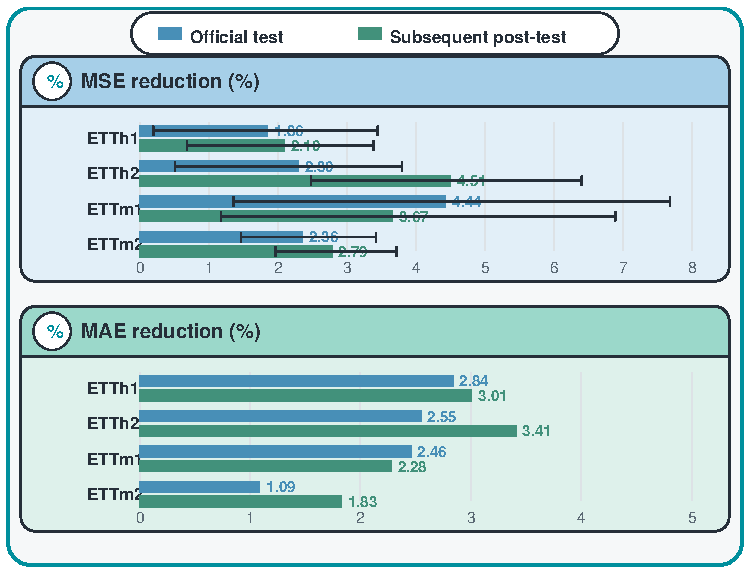
\includegraphics[width=0.65\textwidth]{figures/ett_gains.pdf}
  \caption{Pooled MSE and MAE reductions over matched TimeMixer forecasts
  across three seeds. The post-test timeline is chronologically subsequent to
  the standard split and is excluded from model and correction selection.
  Horizontal lines on MSE bars are 95\% paired moving-block-bootstrap
  intervals. Higher is better.}
  \label{fig:ett-gains}
\end{figure*}

\begin{table*}[h]
\centering
\small
\caption{Pooled MSE reductions and 95\% paired moving-block-bootstrap
intervals. Intervals are candidate-minus-baseline MSE, so values below zero
favor \method{}.}
\label{tab:ett-confidence}
\begin{tabular}{lrrrr}
\toprule
& \multicolumn{2}{c}{Official test} &
\multicolumn{2}{c}{Subsequent post-test}\\
\cmidrule(lr){2-3}\cmidrule(lr){4-5}
Dataset & Reduction & 95\% interval & Reduction & 95\% interval\\
\midrule
ETTh1 & 1.86\% & $[-0.013169,-0.000768]$ &
2.10\% & $[-0.017964,-0.003646]$\\
ETTh2 & 2.30\% & $[-0.011055,-0.001485]$ &
4.51\% & $[-0.011830,-0.004583]$\\
ETTm1 & 4.44\% & $[-0.024903,-0.004411]$ &
3.67\% & $[-0.034576,-0.005918]$\\
ETTm2 & 2.36\% & $[-0.006030,-0.002587]$ &
2.79\% & $[-0.004747,-0.002511]$\\
\bottomrule
\end{tabular}
\end{table*}

\begin{table*}[h]
\centering
\small
\setlength{\tabcolsep}{4pt}
\caption{Per-seed MSE reductions (\%) for the ETT prequential
study. All corresponding MAE values also improve.}
\label{tab:ett-seeds}
\begin{tabular}{lrrrrrr}
\toprule
& \multicolumn{3}{c}{Official test} &
\multicolumn{3}{c}{Subsequent post-test}\\
\cmidrule(lr){2-4}\cmidrule(lr){5-7}
Dataset & 2021 & 2022 & 2023 & 2021 & 2022 & 2023\\
\midrule
ETTh1 & 1.59 & 1.49 & 2.48 & 2.39 & 2.08 & 1.84\\
ETTh2 & 4.31 & 1.18 & 1.37 & 6.29 & 3.69 & 3.49\\
ETTm1 & 2.72 & 8.35 & 2.06 & 2.12 & 5.50 & 3.39\\
ETTm2 & 2.36 & 2.54 & 2.17 & 2.62 & 2.72 & 3.02\\
\bottomrule
\end{tabular}
\end{table*}

The intervals use 5,000 moving-block bootstrap resamples of length 96 after
averaging aligned seed losses at each origin. The later timeline begins on
2018-02-21 for ETTh and ends on 2018-06-25 for ETTm. ETTh uses the fixed stack
specified in the experiment protocol; ETTm retrieval adds an official-test
residual only after its target interval has elapsed.



\end{document}
